% !TeX encoding = UTF-8
% !TeX spellcheck = en_GB

%%% Add [final] option to the report class to switch between draft and final version of the report
%%% Use [narrowmargin] to enable narrow margins - this may impair readability.
%\documentclass[a4paper,12pt,draft]{include/intocpsreport}   %Or
\documentclass[a4paper,12pt,final]{include/intocpsassociation}   %Or
% intocpslargereport if chapters are required.
%
%
%
\usepackage[T1]{fontenc}
\usepackage[utf8]{inputenc}
\usepackage{longtable}
\usepackage{tikz-uml}
\usepackage{framed}
\usepackage{subcaption}
\usepackage[hyphenbreaks]{breakurl}
\usepackage{color}
\usepackage{amsmath}
\usepackage{courier}
\usepackage{xspace}
\usepackage{cleveref}
\usepackage{subcaption}
\usepackage{textcomp} % Used for 20-sim section \textrightarrow
%\usepackage{showframe}

\usepackage{listings}
%% listings-modelica.cfg
%% Copyright 2014 Martin Sjoelund, Dietmar Winkler
%
% This work may be distributed and/or modified under the
% conditions of the LaTeX Project Public License, either version 1.3
% of this license or (at your option) any later version.
% The latest version of this license is in
%   http://www.latex-project.org/lppl.txt
% and version 1.3 or later is part of all distributions of LaTeX
% version 2005/12/01 or later.
%
% This work has the LPPL maintenance status `maintained'.
%
% The Current Maintainer of this work is Dietmar Winkler
%
% Code repository https://github.com/modelica-tools/listings-modelica
%
% This work consists of the file listings-modelica.cfg

\lstdefinelanguage{modelica}
{
  morekeywords=[1]{
    algorithm,and,annotation,as,assert,block,break,case,class,connect,connector,
    constant,constrainedby,der,discrete,each,else,elseif,elsewhen,encapsulated,
    end,enumeration,equality,equation,expandable,extends,external,failure,final,
    flow,for,function,guard,if,import,in,initial,inner,input,List,local,loop,
    match,matchcontinue,model,not,operator,Option,or,outer,output,package,parameter,
    partial,protected,public,record,redeclare,replaceable,return,stream,
    subtypeof,then,Tuple,type,uniontype,when,while},
  morekeywords=[2]{true, false},
  % Do not make true,false keywords because fn(true,x, false ) shows up as fn(true,x, *false*)
  sensitive=true,
  comment=[l]//,
  morecomment=[s]{/*}{*/},
  alsodigit={.,-},
  morestring=[b]',
  morestring=[b]",
}[keywords,comments,strings]

\definecolor{keywordcolor1}{rgb}{0,0,.4}
\definecolor{keywordcolor2}{rgb}{.90,0,0}
\definecolor{stringcolor}{rgb}{0.133,0.545,0.133}
% \definecolor{listingbgcolor}{rgb}{0.95,0.95,0.95}

\lstset{
	frame=trBL,
  breaklines=true,
  language=modelica,
  basicstyle=\ttfamily,
  keywordstyle=[1]\color{keywordcolor1}\bfseries,
  keywordstyle=[2]\color{keywordcolor2},
  stringstyle=\color{stringcolor},
%  backgroundcolor=\color{listingbgcolor},
  framexleftmargin=5mm,
  frameround=fttt,
  xleftmargin=5mm,
  xrightmargin=5mm,
  showstringspaces=false,
}

\lstset{breaklines=true,label=}
% \lstset{basicstyle=\ttfamily}

\newcommand{\code}[1]{\texttt{\hyphenchar%
\font45%
\sloppy%
\fontdimen2\font=0.4em%
\fontdimen3\font=0.2em%
\fontdimen4\font=0.1em%
\fontdimen7\font=0.1em%
 #1}}
 
 


% The VDMlisting package loads the times package which changes the font so we just mark it as loaded to prevent the load. 
\makeatletter
\@namedef{ver@times.sty}{}% a fake for a "loaded" package
\makeatother
\usepackage{vdmlisting}

%% Define listing environment for XML
\definecolor{gray}{rgb}{0.4,0.4,0.4}
\definecolor{darkblue}{rgb}{0.0,0.0,0.6}
\definecolor{cyan}{rgb}{0.0,0.6,0.6}

\lstset{
  basicstyle=\footnotesize\ttfamily,
  columns=fullflexible,
  showstringspaces=false,
  commentstyle=\color{gray}\upshape
}

\lstdefinelanguage{XML}
{
  morestring=[b]",
  morestring=[s]{>}{<},
  morecomment=[s]{<?}{?>},
  stringstyle=\color{black},
  identifierstyle=\color{darkblue},
  keywordstyle=\color{cyan},
  morekeywords={xmlns,version,type}% list your attributes here
}


\lstnewenvironment{xml}[1][]{\lstset{  language=XML,
  morekeywords={encoding, xs:schema,xs:element,xs:complexType,xs:sequence,xs:attribute}}\lstset{#1}}
{}

%% end listing environment for XML
%
%
%
\def\draftnote#1{\noindent\smallskip\framebox{\begin{minipage}{0.95\columnwidth}\color{red}#1\end{minipage}}\smallskip\par}
\newenvironment{draftnoteenv}{\noindent\smallskip\begin{framed}\begin{minipage}{0.95\columnwidth}\color{red}}{\end{minipage}\end{framed}\smallskip\par}
\newenvironment{assumption}{\noindent\smallskip\color{blue}\begin{framed}\begin{minipage}{0.95\columnwidth}}{\end{minipage}\end{framed}\smallskip\par}
%
%
%
\newcommand{\revisit}[1]{\textcolor{red}{\pmb{[[[}\@ #1\@ \pmb{]]]}}}
\newcommand{\intoapp}{INTO-CPS Application}
\newcommand{\into}{INTO-CPS\xspace}
%
%
%\reportnumber{D4.3a}
\reporttitle{INTO-CPS Tool Chain User Manual}
%\reporttitle{User Manual for the INTO-CPS Tool Chain}
\shortreporttitle{INTO-CPS Tool Chain User Manual}  %To use if report title is too long for header
%
%
%
%%% Set document release class as appropriate
%%% e.g. Public, Restricted, Programme Participant
\reportstatus{Public}
%
%
%
%%% If document is a deliverable, this flag should be commented out 
%%% e.g. %\technotetrue
%%% If report is a technical report, leave uncommented
%%% e.g. \technotetrue
%\technotetrue % Comment out as appropriate
%
%
%
\submissiondate{September, 2018}
\contributors{
Victor Bandur, AU\\
Peter Gorm Larsen, AU\\ 
Kenneth Lausdahl, AU \\
Casper Thule, AU\\
Carl Gamble, UNEW\\
Richard Payne, UNEW\\
Adrian Pop, LIU\\
Etienne Brosse, ST\\
J{\"o}rg Brauer, VSI\\
Florian Lapschies, VSI\\
Marcel Groothuis, CLP\\
Tom Bokhove, CLP\\
Christian Kleijn, CLP\\
Luis Diogo Couto, UTRC\\
Christian K\"{o}nig, TWT
}
%
%
%
\editors{
  Peter Gorm Larsen, AU
}
%
%
%
%\reviewers{Ken Pierce, UNEW\\
%Kangfeng Ye, UY\\
%Luis Diogo Couto, UTRC}
%
%
%
%% Version details  
% #1: version
% #2: date
% #3: author
% #4: description
\addversion{0.01}{11-01-2017}{Victor Bandur}{Initial version.}
\addversion{0.02}{30-10-2017}{Victor Bandur}{Updates for internal review.}
\addversion{0.03}{30-10-2017}{Marcel Groothuis}{Added 20-sim 4C FMI import/export manual.}
\addversion{0.04}{12-12-2017}{Marcel Groothuis}{Address internal review comments 20-sim and 20-sim 4C sections.}
\addversion{1.0}{18-12-2017}{Victor Bandur}{Final version inside the INTO-CPS project.}
\addversion{1.1}{26-02-2018}{Peter Gorm Larsen}{First version in the INTO-CPS association.}
\addversion{1.2}{26-09-2018}{Peter Gorm Larsen}{Added material from Fortiss.}

%
%
\begin{document}
\maketitle
%
%
%
%%%% Document abstract page %%%% 
\section*{Abstract}
\label{sec:abstract}
%
This user manual for the INTO-CPS tool chain, an update of Deliverable D4.3a \cite{INTOCPSD4.3a} that was developed inside the INTO-CPS H2020 project and it is now taken further inside the INTO-CPS association.
%
It is targeted at those wishing to make use of the INTO-CPS technology to design and validate cyber-physical systems.
%
This user manual is concerned with those aspects of the tool chain relevant to end-users, so it is necessarily high-level.
%
Other deliverables from the INTO-CPS project discuss finer details of individual components, including theoretical foundations (Deliverables D4.3b \cite{INTOCPSD4.3b}, D4.2c \cite{INTOCPSD4.2c}, D4.3c \cite{INTOCPSD4.3c}, D2.3a \cite{INTOCPSD2.3a}, D2.2b \cite{INTOCPSD2.2b}, D2.3b \cite{INTOCPSD2.3b}, D2.3c \cite{INTOCPSD2.3c}), methods and guidelines (Deliverables D3.3a \cite{INTOCPSD3.3a} and D3.6 \cite{INTOCPSD3.6}) and software design decisions (Deliverables D4.3d \cite{INTOCPSD4.3d}, D5.2a \cite{INTOCPSD5.2a}, D5.3c \cite{INTOCPSD5.3c}, D5.3d \cite{INTOCPSD5.3d}, D5.3e \cite{INTOCPSD5.3e}).
%
\newpage
%
%%%% Document table of contents page %%%% 
\tableofcontents
\newpage
%
%
%
%%%% Document Content %%%% 
%% \chapter{Chapter Title} %% if intocpslargereport is in use
%\begin{assumption}
%
%
%
%!TEX root = ../INTO-CPS-Manifesto.tex

\section{Introduction}\label{sec:intro}

%\fbox{Peter Gorm Larsen}

Cyber-Physical Systems (CPSs) present major business and societal
opportunities in a variety of application areas--- \emph{if} they can be developed economically~\cite{Cengarle&13}. Model-Based Development (MBD) has the potential to enhance the development of CPSs, increasing the competitiveness of industry by shortening time to market and reducing development costs. In the interface between disciplines, different formalisms and technical cultures meet, and the traditional approaches for designing systems vary significantly among the relevant fields. Some researchers advocate for describing such hybrid systems using a single formalism/tool \cite{Ptolemaeus14,Platzer18}, but here we believe that it is better to enable stakeholders with different disciplinary backgrounds to produce their constituent models using their preferred formalism/tool and then enable joint analysis using co-simulation \cite{Gomes&18} and ensuring that there is an underlying common foundation for all of them.
Even the proposals for a single \cite{Ptolemaeus14,Platzer18} recognise that one cannot expect different stakeholders to learn the same formalism. Instead, they propose a formalism that integrates multiple sub-formalisms, to ensure that the result can cover a wide range of paradigms.

Different stakeholders can produce constituent models of the parts they are responsible for. The combination of the different constituent models forms the CPS model.
The main challenge is to ensure that such constituent models connect and thus can be combined in different analysis conducted of the behaviour of the CPS in its desired surroundings, typically called its environment.
%\claudio{The prev sentence is also trying to do too much!}
Since the design of the CPSs depends on the ability to connect the behaviours of its constituent models, the main challenge is to make sure these results are trustworthy.
%Different formalisms are usually
%supported by different tools running on different Operating Systems (OSs).

Different research projects have targeted the development of chains of tools which collectively would enable the envisaged combination of different formalisms and tools in the development of CPSs. The DESTECS\footnote{This is an acronym for ``Design Support and Tooling for Embedded Control Software'', see \url{http://destecs.org/}.} project \cite{Broenink&10} combined the Overture/VDM tool \cite{Larsen&10a} with the 20-sim tool \cite{Kleijn06} with a dedicated co-simulation combination with a Crescendo tool \cite{Fitzgerald&14c}. The MODELISAR project\footnote{See \url{https://itea3.org/project/modelisar.html}.} developed an open standard for interfacing between different constituent models called the Functional Mockup Interface (FMI) enabling co-simulation between any tool supporting this standard maintained by the Modelica Association\footnote{See \url{https://www.modelica.org/}.}. The INTO-CPS project\footnote{See \url{http://projects.au.dk/into-cps/}.} took this further with a tool chain going all the way from requirements to final realisations using the FMI standard. This developed the INTO-CPS technology which consists of 1) a common semantic foundation, 2) a methodology with guidelines for the development of CPS and 3) an open tool chain.
\claudio{Maybe you can summarize the above in a table. Maybe as in Table~\ref{tab:projects}.}

\begin{table}[htb]
  \scriptsize
  \caption{Summary of research activities in the field of co-simulation in recent years. \claudio{Taken from a journal paper which has been submitted but not accepted yet. Maybe need to cite it like that\ldots}}
  \label{tab:projects}
  \begin{tabular}{llp{0.55\textwidth}}
  \textbf{Project} & \textbf{Duration} & \textbf{Goals} \\ \hline
  COSIBA~\cite{cosibas} & 2000--2002 &  Formulate a co-simulation backplane for coupling electronic design automation tools,  supporting different abstraction levels. \\
  ODETTE~\cite{odette} & 2000--20003 &  Develop a complete co-design solution including hardware/software co-simulation and synthesis tools. \\
  MODELISAR~\cite{modelisar} & 2008--2011 &  Improve the design of embedded software in vehicles. \\
  DESTECS~\cite{destecs} & 2010--2012 &  Improve the development of fault-tolerant embedded systems. \\
  INTO-CPS~\cite{intocps} & 2015--2017 &  Create an integrated tool chain for Model-Based Design of CPS with FMI.  \\
  ACOSAR~\cite{acosar} & 2015--2018 &  Develop a non-proprietary advanced co-simulation interface for real time system integration.  \\
  OpenCPS~\cite{opencps} & 2015--2018 &  Improve the interoperability between Modelica, UML and FMI.  \\
  ERIGrid~\cite{erigrid} & 2015--2020 &  Propose solutions for Cyber-Physical Energy Systems through co-simulation.  \\
  PEGASUS~\cite{pegasus} & 2016--2019 &  Establish standards for autonomous driving. \\
  CyDER~\cite{cyder} & 2017--2020 &  Develop a co-simulation platform for integration and analysis of high PV penetration. \\
  EMPHYSIS~\cite{emphysis} & 2017--2020 &  Develop a new standard (eFMI) for modeling and simulation environments of embedded systems.  \\ 
  \hline
  \end{tabular}%
\end{table}


Before the end of the INTO-CPS project, the Intellectual Property (IP) developed was transferred to the non-profit INTO-CPS Association\footnote{This is registered as a legal entity in Denmark, see \url{into-cps.org/}.}. The Association maintains and further develops the INTO-CPS technology, and grows the open tool chain by adding additional tools from its partners, while keeping the documentation and tutorial material up to date. 
%It attempts to ensure that the different tools are kept in sync and that the importable examples expressed using diverse notations and tools are kept up to date.
%\claudio{This last sentence seems redundant.}

Since this guide is meant as a general introduction to INTO-CPS it is written such that it should be relatively easy to jump around and read different sections of interest. This guide to INTO-CPS begins with an overview of challenges in the engineering of CPSs in Section~\ref{sec:challenges}. Then Section~\ref{sec:nutshell} provides a short overview of the INTO-CPS project in a nutshell. Section~\ref{sec:foundations} gives an overview of the CPS foundations; Section~\ref{sec:method} gives an overview of the CPS methodology; and Section~\ref{sec:toolchain} an overview of the tool chain. The industrial use of the INTO-CPS technology is summarised in Section~\ref{sec:casestudies}. Finally, Section~\ref{sec:related} provides an overview of related work, and Section~\ref{sec:future} looks at potential future directions for the INTO-CPS technology. 
There are two appendices: Appendix~\ref{appendix:acronyms} provides a list of acronyms,  
%Appendix~\ref{appendix:principles} provides a common definition of the main terms used in the INTO-CPS documentation 
and Appendix~\ref{appendix:tools} is an overview of the individual tools used in the INTO-CPS tool chain.
%There are three appendices: Appendix~\ref{appendix:acronyms} provides a list of acronyms; Appendix~\ref{appendix:principles} provides a common definition of the main terms used in the INTO-CPS documentation and Appendix~\ref{appendix:tools} is an overview of the individual tools used in the INTO-CPS tool chain.

%Systems composed of closely coupled computing and physical elements are becoming increasingly important in the modern world. For society and citizens, the potential of such smart systems to deliver more efficient, sustainable and resilient services is enormous.  Such Cyber-Physical Systems (CPSs) are characterised by a complex architecture and a design process involving several diverse science and engineering disciplines. In the interface between disciplines, different formalisms and technical cultures meet, and the traditional approaches for designing systems vary significantly among the relevant fields.
%\claudio{It's not clear how the previous sentence relates to the next. Is it the cause of the vast design space? It seems to be more related to the two last sentences of this paragraph.}
%The developer of a CPS faces a large design space that is hard to cover with hardware prototypes \claudio{maybe add: and physical experiments} due to the high cost of their implementation. Common workflows to assist the engineering of CPSs with a model-based approach, and the necessary tools, are currently lacking. Different stakeholders can produce models of the parts they are responsible for, and we will call these constituent models that together form the entire CPS.
%
%\claudio{This paragraph seems to be the continuous of the previous one (but the previous one has a gap, and should maybe be splitted).
%Anyhow, the logical workflow is a bit confusing. Maybe we should go bottom up: first explain the there are diverse disciplines, and that each has its methods, formalisms, and jargon, and then explain that these need to interact and collaborate, in order to successfully develop a CPS. This then leads us to the need for into-cps.}
%The design of CPSs involves the usage of results obtained
%using a combination of different formalisms serving different engineering
%disciplines. Different formalisms are usually
%supported by different tools running on different Operating Systems (OSs).
%
%In this manifesto we put forward the idea of combining different formalisms and
%respective supporting tools by means of a tool chain. A tool chain allows the
%practitioner to easily combine the results from the various fields during the
%design process.  Our view is that it is best to enable different disciplinary experts to use the tools they are most familiar with and
%integrating the different constituent models by building an environment automating the tool chain
%interaction, accessibility, and unifying the entry point to it.
%\claudio{If the motivation is clearly provided in the previous paragraphs, then this last sentence should be redundant.}
%
%In such unified environment of several tools, users keep their usual patterns
%of interaction with their familiar tool(s) available in the tool chain.
%\claudio{The next sentence says the same thing as the previous one.}
%Instead of having to learn a new formalism, the different disciplinary experts can stay with the tools they are most familiar with and they find most natural to create the constituent models requires for their work.
%The chain of tools then needs also to enable each individual of seeing the consequences of changes locally in a global context where the other constituent models are incorporated.
%\claudio{I think this paragraph should not need to exist, if the problem is well motivated. These are all pressing needs in the current development of CPS.
%So the logical flow should be ``MOTIVATION (pressing needs) -> Solution (it should be clear why this is a solution, we don't need to justify more)''.}
%
%Naturally, such different constituent models needs to interface to each other and here we make use of a de-facto standard originating in the automotive industry called the Functional-Mockup Interface (FMI).
%\claudio{The next sentence says the same thing as the previous one.}
%Thus, the different tools in the INTO-CPS tool chain are able to interact with other tools directly or indirectly using the FMI standard.
%\claudio{The next couple of sentences seems to be an afterthought. Maybe they should be put in a different paragraph, and the problem that the traceability solves should be described in the motivation section.}
%In order also to be able to trace artefacts from different constituent models and results generated from analysis using different tools another standard called the Open Services for Lifecycle Collaboration (OSLC) is used. This enables seeing and documenting the dependencies between different versions of different constituent models and local or global analysis conducted about them.
%
%\claudio{What's the point of the next sentence?}
%It is hard for a single person to master all the components of the tool chain, but fortunately that is not required.
%The mastering of tool chains involves the management of the whole set
%of models and inputs/results for each of the tools. In addition, the conversion
%of results, traceability of changes and keeping track of the user interactions
%need also to be taken into account.
%\claudio{The next sentence is one of the motivations for the INTO-CPS association\ldots It should be in a paragraph by itself.}
%Moreover, given the evolving nature of
%each of the tools, the task of managing the tool chain while ensuring the
%dependencies of each of the tools and their interoperability becomes too
%complex. The INTO-CPS Association attempts to ensure that the different tools are kept in sync and that the importable examples expressed in a collection of notations using different tools \claudio{Do we need to say ``expressed in a collection of notations using different tools''? That seems redundant.} (these are called multi-models \claudio{We don't need to define a new term here, if we are not going to use it in this section.}) are kept up to date.
%
%%Practice shows users are more receptive to a  push-button approach when it is
%%time to combine their results with the other tools.
%
%\claudio{Why did we switch from talking about the into-cps association, to the into-cps tool?
%Why not start with the tecnology, and end with the into-cps association? Because we start with the tecnological problems\ldots}
%The INTO-CPS technology builds upon a frontend application which was developed following the
%unified entry point idea.  The INTO-CPS application allows the user to fetch
%the different tools, checkout multi-models from repositories, orchestrate the
%several tools run, and organise the results/interactions.  This reduces the
%challenges of mastering the complexity essentially to a push-button effort when the multi-models have been produced by different disciplinary experts.
%



\clearpage
\section{Overview of the INTO-CPS Tool Chain}\label{sec:overview}
The INTO-CPS tool chain consists of several special-purpose tools from a number of different providers.
%
Note that this is an open tool chain, so it is possible to incorporate other tools that also support the FMI standard for co-simulation.
%
We have already tested this with numerous external tools (both commercial as well as open-source).
%
The constituent tools are dedicated to the different phases of collaborative modelling activities.
%
They are discussed individually through the course of this manual.
%
An overview of the tool chain is shown in Figure \ref{figure:toolchainoverview}.
%
%
%
\begin{figure}[ht]
\centering
% !TeX root=../D4.1a_User_Manual.tex
\usetikzlibrary{positioning,fit,calc}
\usetikzlibrary{arrows}
\usetikzlibrary{decorations.pathreplacing}
\makeatletter
\tikzset{%
  show node name/.code={%
    \expandafter\def\expandafter\tikz@mode\expandafter{\tikz@mode\show\tikz@fig@name}%
    }
}

\def\toolfmu#1#2#3{

\node[myBox,#2,myGray] (#1ovtToolWrapper){\parbox{2.5cm}{\centering Tool Wrapper\\#3}};
\node[myBox,#2, left=of #1ovtToolWrapper,myGray] (#1ovtNative){\parbox{2.5cm}{\centering Generated Native\\#3}};
\coordinate (#1ovtToolWrapper-#1ovtNative) at ($(#1ovtToolWrapper)!0.5!(#1ovtNative)$);
\node[myBox, below=of #1ovtToolWrapper-#1ovtNative,fill=orange!10] (#1model) {\parbox{2.5cm}{\centering Model\\+\\#3
%\includegraphics[width=.25\textwidth]{Overture-logo.png}
}    
};
\node[draw,dashed,fit=(#1ovtToolWrapper) (#1ovtNative) (#1model), ] (#1fmugroup) {\footnotesize Tool specific};

\draw[draw,-triangle 90,dotted] (#1model.west) to[out=170,in=270,looseness=2]node [midway, below, sloped]   {\scriptsize Generate} (#1ovtNative.south) ;
\draw[draw,-triangle 90,dotted] (#1ovtToolWrapper.south) to[out=170,in=0,looseness=2]node [midway, above, sloped]   {\scriptsize Using} (#1model.east) ;
 

} 

\begin{tikzpicture}[scale=0.55, transform shape]
\tikzset{myFont/.style={font=\footnotesize}}
\tikzset{myBox/.style={draw,minimum height=1cm,minimum width=2cm,myFont}}
\tikzset{myGray/.style={fill=gray!10}}
\tikzset{myBlue/.style={draw=blue!60}}
\tikzset{tool/.style={dotted,draw,minimum size=2.5cm}}
\tikzset{fmu/.style={draw,minimum width=2.5cm,minimum height=1cm}}


\node[tool](modelio) {\parbox{3cm}{
\includegraphics[width=2cm]{figures/logo-modeliosoft.png} \\ \centering Modelio}};

%\node[tool, above right= 3cm of modelio](mc) {Model Checking};

\node[myBox, below= 2cm of modelio](md) {Model Description};

\node[tool, below left=2.8cm of md](overture) {\parbox{3cm}{
\includegraphics[width=2cm]{figures/Overture_icon_128x128.png} \\ \centering Overture}};

\node[tool, right=of overture](20sim) {\parbox{3cm}{
\includegraphics[width=2cm]{figures/20simIconWithShadow48.jpg} \\ \centering 20-sim}};

\node[tool, right=of 20sim](om) {\parbox{3cm}{
\includegraphics[width=2cm]{figures/omediticon.png} \\ \centering OpenModelica}};

\node[tool, right=of om](rttester) {\parbox{3cm}{
\includegraphics[width=2cm]{figures/verified.jpeg} \\ \centering RT-Tester}};


\node[fmu, below=1.8cm of overture](fmuOverture){FMU};
\node[fmu, right=of fmuOverture](fmu20sim){FMU};
\node[fmu, right=of fmu20sim](fmuOm){FMU};
\node[fmu, right=of fmuOm,xshift = 0.6cm,yshift = -0.6cm,fill=white](fmuRttester2){   };
\node[fmu, right=of fmuOm,xshift = 0.3cm,yshift = -0.3cm,fill=white](fmuRttester1){   };

\node[fmu, right=of fmuOm,fill=white](fmuRttester){FMU};



\node[dashed,draw,transform shape=false,fit=(fmuOverture) (fmu20sim) (fmuOm) (fmuRttester) (fmuRttester1) (fmuRttester2)] (fmu) {};
%\node [anchor=north west] at (cosim.north west) {\underline{Simulation}};

% links
 \draw[draw,-triangle 90, ]
	(modelio) -- (md) node [midway, above, sloped]  {Export part};

% imports	
 \draw[draw,-triangle 90, ]
	(overture) -- (md) node [midway, above, sloped]  {Import};
 \draw[draw,-triangle 90, ]
	(20sim) -- (md) node [midway, above, sloped]  {Import};
 \draw[draw,-triangle 90, ]
	(om) -- (md) node [midway, above, sloped]  {Import};
 \draw[draw,-triangle 90, ]
	(rttester) -- (md) node [midway, above, sloped]  {Import};
	
% fmu export
 \draw[draw,-triangle 90, ]
	(overture) -- (fmuOverture) node [midway, above, sloped]  {Export};
 \draw[draw,-triangle 90, ]
	(20sim) -- (fmu20sim) node [midway, above, sloped]  {Export};
 \draw[draw,-triangle 90, ]
	(om) -- (fmuOm) node [midway, above, sloped]  {Export};
 \draw[draw,-triangle 90, ]
	(rttester) -- (fmuRttester) node [midway, above, sloped]  {Export};
	
% fmu import
\draw[draw,-triangle 90,overlay] (fmu.west) to[out=120,in=180,looseness=1]node [midway, above, sloped]  {FMU Import} (modelio.west);

% overture uml connection
 \draw[draw,-triangle 90, ]
	(overture) -- (modelio) node [midway, above, sloped]  {UML Model Exchange};

\node[myBox, right=5cm of modelio](app){\parbox{2cm}{\centering INTO-CPS App}};

\node[myBox, right=2cm of app](dse){DSE};

\node[myBox, right=2cm of dse](coe){COE};

% obtain config
% \draw[draw,-triangle 90, ]
%	(mc) -- (rttester) node [midway, above, sloped]  {Model Check?};
	
\draw[draw,-triangle 90] ($(rttester.south)-(-0.9,0)$) to[out=315,in=345,looseness=10]node [midway, below, sloped]  {FMU Model Check} ($(rttester.south east)+(-0,0.9)$);

\draw[draw,-triangle 90] ($(rttester.north east)-(-0,1.2)$) to[out=15,in=60,looseness=5]node [midway, above, sloped]  {Co-sim Model Check} ($(rttester.north)-(-0.9,0.0)$) ;
	
%dse links


\draw[draw,-triangle 90] (app.north east) to[out=90,in=90,looseness=1.5]node [midway, above, sloped]  {\parbox{2cm}{Co-sim config}} (dse.north west);
\draw[draw,-triangle 90] (dse.south west) to[out=270,in=270,looseness=1.5]node [midway, below, sloped]  {\parbox{2cm}{\centering Optimal co-sim config}} (app.south east);

\draw[draw,-triangle 90] (dse.north) to[out=90,in=90,looseness=1.5]node [midway, above, sloped]  {\parbox{2cm}{Co-sim config}} (coe.north west);
\draw[draw,-triangle 90] (coe.south west) to[out=270,in=270,looseness=1.5]node [near end, above, sloped]  {} (dse.south);
	
	
\draw[draw,-triangle 90,myBlue] (app.north) to[out=90,in=90,looseness=1.5]node [midway, above, sloped]  {\parbox{2cm}{Co-sim config}} (coe.north);
\draw[draw,-triangle 90,myBlue] (coe.south) to[out=270,in=270,looseness=1.5]node [near end, above, sloped]  {} (app.south);

%app update link
\draw[draw,-triangle 90] ($(app.south)+(-0.9,0)$) to[out=290,in=210,looseness=55]node [midway, below, sloped]  {Live Update} (app.south west);
%\draw (app.south west) to [out=330,in=300,looseness=8] (app.south west);

%model check link
 \draw[draw,-triangle 90, ]
	(app) -- (modelio) node [midway, above, sloped]  {Obtain co-sim config};


\end{tikzpicture}
\caption{Overview of the structure of the INTO-CPS tool chain.}
\label{figure:toolchainoverview}
\end{figure}
%
%
%
The main interface to INTO-CPS is the \intoapp.
%
This is where the user can design co-simulations from scratch, assemble them using existing FMUs and configure how simulations are executed.
%
The result is a \emph{multi-model}.
%
The multi-model can then be analysed through co-simulation, model checking and model-based testing.

The design of a multi-model is carried out visually using the Modelio SysML tool, in accordance with the SysML/INTO-CPS profile described in D2.3a \cite{INTOCPSD2.3a}.
%
Here one can either design a multi-model from scratch by specifying the characteristics and connection topology of Functional Mockup Units (FMUs) yet to be developed, or import existing FMUs so that the connections between them may be laid out visually.
%
The result is a SysML architecture model of the multi-model, expressed in the SysML/INTO-CPS profile.
%
In the former case, where no FMUs exist yet, a number of \texttt{model\allowbreak{}Description\allowbreak{}.xml} files are generated from this multi-model which serve as the starting point for constituent model construction inside each of the individual simulation tools, leading to the eventual FMUs.

Once a multi-model has been designed and populated with concrete FMUs, the Co-simulation Orchestration Engine (COE) can be invoked to execute a co-simulation.
%
The COE controls all the individual FMUs in order to carry out the co-simulation.
%
In the case of tool-wrapper FMUs, the model inside each FMU is simulated by its corresponding simulation tool.
%
The tools involved are Overture \cite{Larsen&10a}, 20-sim \cite{20sim} and OpenModelica \cite{OpenModelica}.
%
RT-Tester is not under the direct control of the COE at co-simulation time, as its purpose is to carry out testing and model checking rather than simulation.
%
The user can configure a co-simulation, for instance by running it with different simulation parameter values and observing the effect of the different values on the co-simulation outcome.

Alternatively, the user has the option of exploring optimal simulation parameter values by entering a DSE phase.
%
In this mode, ranges are defined for various parameters which are explored, in an intelligent way, by a design space exploration engine that searches for optimal parameter values based on defined optimization conditions.
%
This engine interacts directly with the COE and itself controls the conditions under which the co-simulation is executed.

The Domain Specific Language Configuring HLA (CoHLA) for constructing a co-simulation from a set of simulation models uses the High Level Architecture (HLA) standard for the coordination of a co-simulation.

\clearpage
\section{The INTO-CPS Application}\label{sec:app}
This section describes the \intoapp{}, the primary gateway to the \into tool chain.
%
Section \ref{sub:introduction} gives an introductory overview of the \intoapp{}.
%
Section \ref{sub:projects} describes how the \intoapp{} can be used to create new INTO-CPS co-simulation projects.
%
Section \ref{sub:multi-models} describes how multi-models can be assembled.
%
Section \ref{sec:co-simulations} describes how co-simulations are configured, executed and visualized.
%
Section \ref{sub:other-features} lists some additional useful features of the \intoapp{}, while Section \ref{sec:COE} describes how the co-simulation engine itself can be started manually, for specialist use.
%
%
%
\subsection{Introduction}
\label{sub:introduction}

The \intoapp{} is the front-end of the entire \into tool chain.
%
The \intoapp{} defines a common \into project and it is the easiest way to configure and execute co-simulations.
%
Certain features in the tool chain are only accessible through the \intoapp{}.
%
Those features will be explained in their own sections of the user manual.
%
This section introduces the \intoapp{} and its basic features only.

Releases of the \intoapp{} can be downloaded from:
%
%
%
\begin{quote}
  \url{https://into-cps-association.github.io/into-cps/download}
\end{quote}
%
%
% 
Five variants are available:
%
%
%
\begin{itemize}
  \item \texttt{-darwin-x64.zip} -- MacOS version
  \item \texttt{-linux-ia32.zip} -- Linux 32-bit version
  \item \texttt{-linux-x64.zip} -- Linux 64-bit version
  \item \texttt{-win32-ia32.zip} -- Windows 32-bit version
  \item \texttt{-win32-x64.zip} -- Windows 64-bit version
\end{itemize}
%
%
%
The \intoapp{} itself has no dependencies and requires no installation. Simply unzip it and run the executable. However, certain \intoapp{} features require
Git\footnote{\url{https://git-scm.com/}}, Java
8\footnote{\url{http://www.oracle.com/technetwork/java/javase/overview/java8-2100321.html}} and Python 2\footnote{\url{http://www.python.org/downloads/}} to be already installed.

The main window of the \intoapp{}, with a project already loaded, is shown in Figure \ref{fig:app-main}.
%
The left panel shows the \into project explorer.
%
The central area of the window displays the contents of the current project's README file.
%
The bottom of the main \intoapp{} window contains two navigation tabs.
%
When clicked, their content is displayed immediately above.
%
Figure \ref{fig:app-main} shows this for the ``COE Console'' tab.
%
Elements of the main window are discussed in further detail below.
%
The tabs are as follows:
%
%
%
\begin{itemize}
\item  ``COE Console'' shows the output of the COE process and log messages with a log level of ``error'' or ``warning''. Furthermore, a dot shows whether the COE is online or offline. If the dot is green then the COE is online, whereas the dot is red when the COE is offline.  The ``Launch'' and ``Stop'' buttons start and stop the COE process, respectively.  If ``Stream Redirect'' is followed by a link icon (
\includegraphics[width=0.1in]{./figures/app/link}) then the output of the COE is shown in this part of the main window, otherwise no COE output is shown.
%
\item  ``COE log'' shows the co-simulation log output according to the co-simulation configuration.
\end{itemize}
%
%
%
\begin{figure}[ht]
\centering
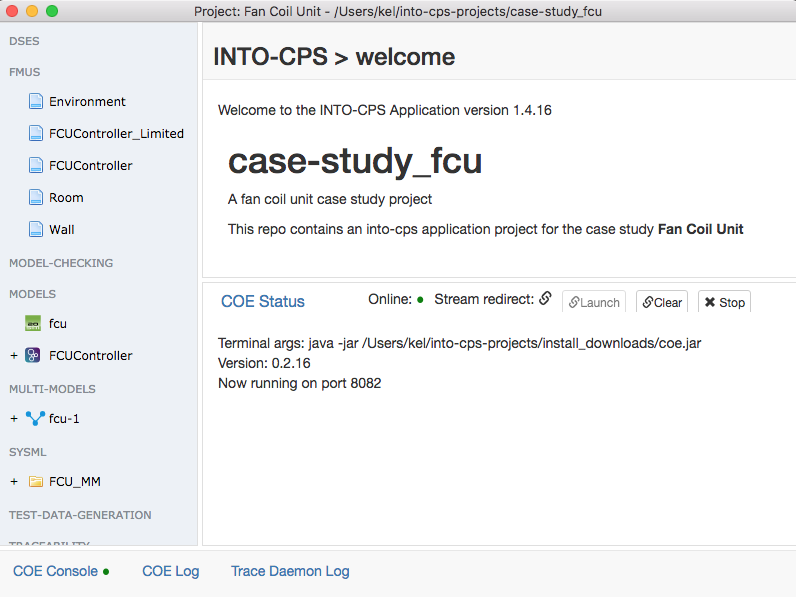
\includegraphics[width=\textwidth]{./figures/app/main}
\caption{\intoapp{} main window.}
\label{fig:app-main}
\end{figure}
%
%
%
\subsection{Projects}
\label{sub:projects}
An \into project contains all the artifacts used and produced by the tool
chain. The project artifacts are grouped into folders. You can create as
many folders as you want and they will all be displayed in the project browser.
The default set of folders for a new project, shown in Figure \ref{fig:app-proj}, is:
%
%
%
\begin{figure}[ht]
\centering
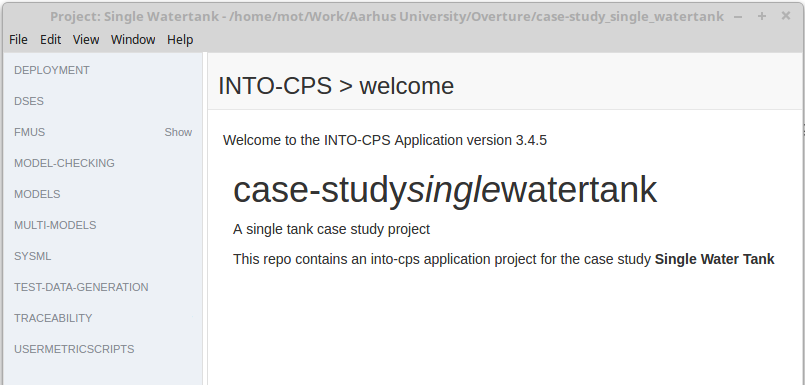
\includegraphics[width=0.85\textwidth]{./figures/app/projbrowser}
\caption{\into project shown in the project browser.}
\label{fig:app-proj}
\end{figure}
%
%
%
\begin{description}
  \item[DSES] Scripts and configuration files for
    performing DSE experiments.
  \item[FMUs] FMUs for the constituent models of the project.
  \item[Model-Checking] Configuration files for performing Model Checking experiments.
  \item[Models] Sources for the  constituent models of the project.
  \item[Multi-Models] The multi-models of the project, using the project FMUs. This
    folder also holds configuration files for performing co-simulations.
  \item[SysML] Sources for the SysML model that defines the architecture and
    connections of the project multi-model. 
  \item[Test-Data-Generation] Configuration files for performing test data
    generation experiments.
  \item[Traceability]  Traceability-specific files plus context menu for traceability information.
  \item[userMetricScripts]  Data analysis scripts.
\end{description}
%
%
%
In order to create a new project, select \textit{File} $\rightarrow$ \textit{New Project}, as shown
in Figure \ref{fig:newproj-menu}. This opens the dialog shown in
Figure \ref{fig:newproj-diag}, where you must choose the project name and location -- the chosen location will be the root of the project, so you should manually
create a new folder for it.
%
%
%
\begin{figure}
  \centering
  \begin{subfigure}[b]{0.45\textwidth}
    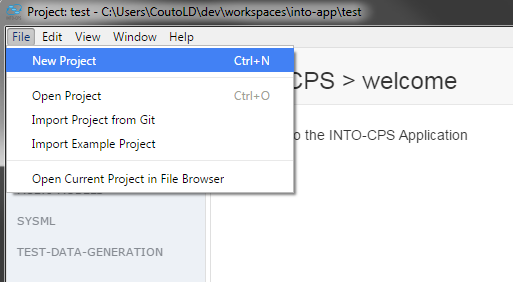
\includegraphics[width=\textwidth]{figures/app/newproj-menu}
    \caption{\emph{New Project} menu entry.}
    \label{fig:newproj-menu}
  \end{subfigure}
  \quad 
  \begin{subfigure}[b]{0.45\textwidth}
    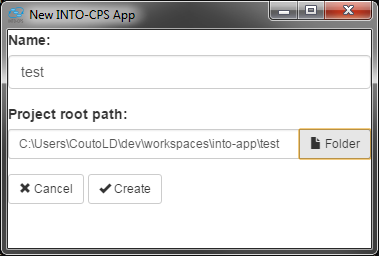
\includegraphics[width=\textwidth]{figures/app/newproj-diag}
    \caption{\emph{New Project} dialog.} 
    \label{fig:newproj-diag}
  \end{subfigure}
  \caption{Creating a new INTO-CPS project.}
  \label{fig:newproj}
\end{figure}
%
%
%
To open an existing project, select \textit{File} $\rightarrow$ \textit{Open Project}, then navigate to the project's root folder and open it. 

To import a project stored in the Git version control system, select
\textit{File} $\rightarrow$ \emph{Import Project from Git}, as shown in Figure \ref{fig:gitproj-menu}.
This opens the dialog shown in Figure \ref{fig:gitproj-diag}, where you must
choose the project location and also provide the Git URL. The project is checked
out using Git, so any valid Git URL will work. You must also have Git available
in your PATH environment variable in order for this feature to work.
%
%
%
\begin{figure}
\centering
\begin{subfigure}[b]{0.45\textwidth}
  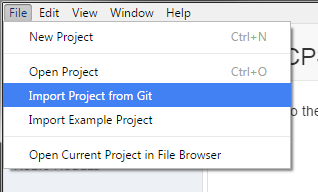
\includegraphics[width=\textwidth]{figures/app/gitproj-menu}
  \caption{\emph{Import Git Project} menu entry.}
  \label{fig:gitproj-menu}
\end{subfigure}
\quad 
\begin{subfigure}[b]{0.45\textwidth}
  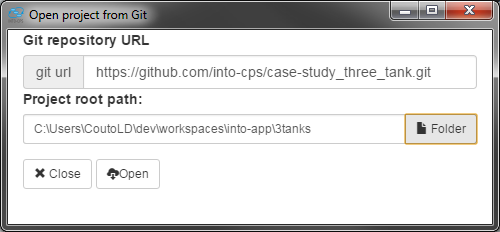
\includegraphics[width=\textwidth]{figures/app/gitproj-diag}
  \caption{\emph{Import Git Project} dialog.} 
  \label{fig:gitproj-diag}
\end{subfigure}
\caption{Importing a Git project.}
\label{fig:gitpro}
\end{figure}
%
%
%
It is possible to import several public example projects that show off
the various features of the \into tool chain. These examples
are described in Deliverable D3.6 \cite{INTOCPSD3.6}. To import an example, select
\textit{File} $\rightarrow$ \emph{Im\-port\ Ex\-amp\-le\ Pro\-ject}, as shown in Figure \ref{fig:example-menu}.
This opens the dialog box shown in Figure \ref{fig:example-diag}, where you 
must select which example to import and a project location. The example
is checked out via Git, so you must have Git available in your path in order
for this feature to work.
%
%
%
\begin{figure}[h!]
\centering
\begin{subfigure}[b]{0.45\textwidth}
  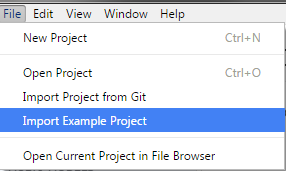
\includegraphics[width=\textwidth]{figures/app/example-menu}
  \caption{\emph{Import Example Project} menu.}
  \label{fig:example-menu}
\end{subfigure}
\quad 
\begin{subfigure}[b]{0.45\textwidth}
  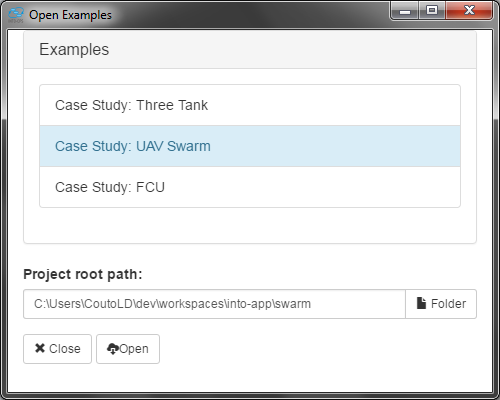
\includegraphics[width=\textwidth]{figures/app/example-diag}
  \caption{\emph{Import Example Project} dialog.} 
  \label{fig:example-diag}
\end{subfigure}
\caption{Importing examples.}
\label{fig:example}
\end{figure}
%
%
%
For both Git projects and examples, once you begin the import process,
a process dialog is displayed, as shown in Figure \ref{fig:git-prog}.

\begin{figure}[ht]
\centering
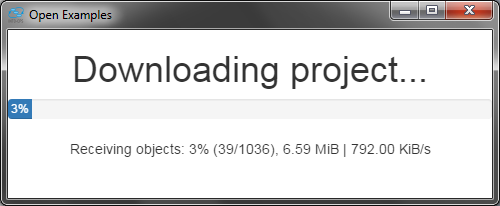
\includegraphics[width=0.45\textwidth]{./figures/app/git-prog}
\caption{Progress of project imports through Git.}
\label{fig:git-prog}
\end{figure}
%
%
%
\subsection{Multi-Models}
\label{sub:multi-models}
For any given project, the \intoapp{} allows you to create and edit multi-models and
co-simulation configurations. To create a new multi-model, right click the
\textit{Multi-models} node in the project browser and select  \textit{New
multi-model}, as shown in Figure \ref{fig:new-mm}. After creation, the new
multi-model is automatically opened for editing.
%
%
%
\begin{figure}[h!]
\centering
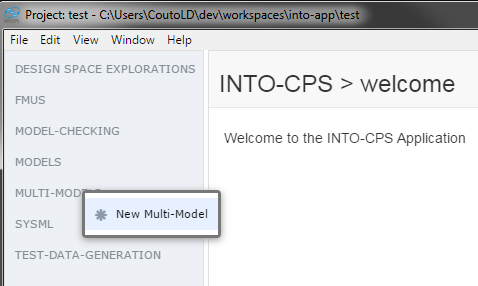
\includegraphics[width=0.65\textwidth]{./figures/app/new-mm}
\caption{Creating a new multi-model.}
\label{fig:new-mm}
\end{figure}
%
%
%
To select an existing multi-model for editing, double-click it. 
Once a multi-model is open, the multi-model view, shown in
Figure \ref{fig:mm-view} is displayed. The top box, \textit{Overview},
displays an overview of the input and output variables in the FMUs,
as shown in Figure \ref{fig:mm-overview}. The bottom box, \textit{Configuration}, enables the user to configure the multi-model.
%
%
%
\begin{figure}[h!]
\centering
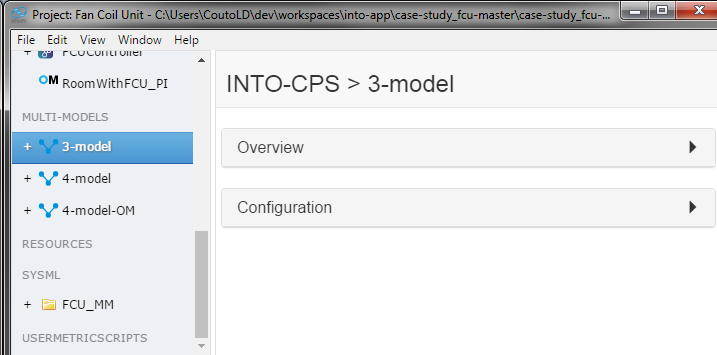
\includegraphics[width=0.75\textwidth]{./figures/app/mm-view}
\caption{Main multi-model view.}
\label{fig:mm-view}
\end{figure}
%
%
%
\begin{figure}[h!]
\centering
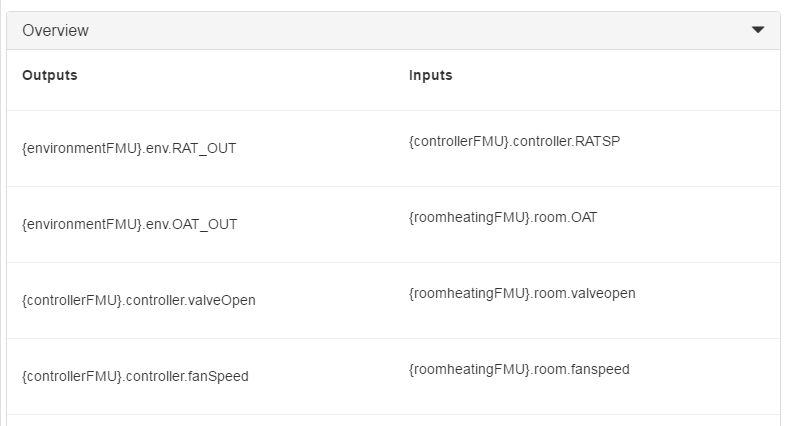
\includegraphics[width=\textwidth]{./figures/app/mm-overview}
\caption{Multi-model overview.}
\label{fig:mm-overview}
\end{figure}
%
%
%
In order to configure a multi-model, it must first be unlocked for editing
by clicking the \textit{Edit} button at the bottom of the \textit{Configuration}
box. There are four main areas dedicated to configuring various aspects of a multi-model.

The \textit{FMUs} area, shown in Figure \ref{fig:mm-fmus}, allows you to remove or add
FMUs and to associate the FMUs with their files by browsing to,
or typing, the path of the FMU file. For each FMU file a marker is
displayed indicating whether the FMU is supported by the \intoapp{} and can be used for co-simulation on the current platform.
%
%
%
\begin{figure}[h!]
\centering
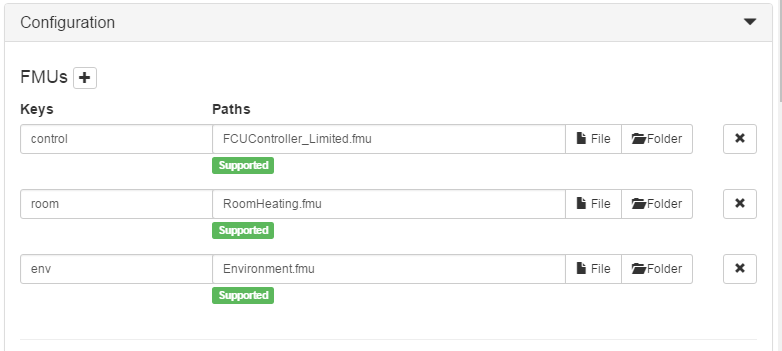
\includegraphics[width=0.9\textwidth]{./figures/app/mm-fmus}
\caption{FMUs configuration.}
\label{fig:mm-fmus}
\end{figure}
%
%
%
The \textit{FMU instances} area, shown in Figure \ref{fig:mm-instances}, allows you to
create or remove FMU instances and name them. A multi-model consists of one or more interconnected instances of various FMUs. More than one instance may be created for a given FMU.
%
%
%
\begin{figure}[h!]
\centering
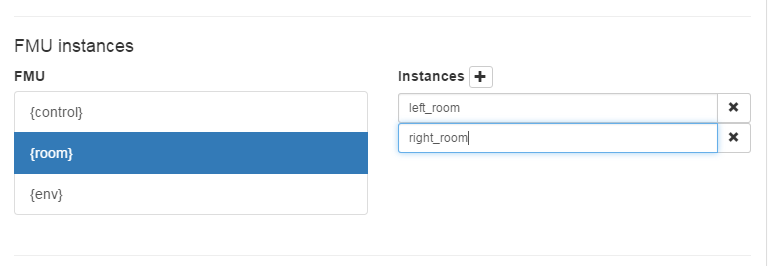
\includegraphics[width=0.9\textwidth]{./figures/app/mm-instances}
\caption{FMU instances configuration.}
\label{fig:mm-instances}
\end{figure}
%
%
%
As a convenient workflow shortcut, the \textit{Connections} area, shown in Figure \ref{fig:mm-conns}, allows you to
connect output variables from an FMU instance into input variables of another:

\begin{enumerate}
  \item Click the desired output FMU instance in the first column.  The output variables for the selected FMU appear in the second column.
  \item Click the desired output variable in the second column.  The input instances appear in the third column.
  \item Click the desired FMU input instance in the third column.  The input variables for the selected FMU appear in the fourth column.
  \item Check the box for the desired input variable in the fourth column.
\end{enumerate}
%
%
%
This facility makes it unnecessary to return to Modelio whenever small changes must be made to the connection topology of the multi-model\footnote{Changes made to a multi-model or FMU outside of the \intoapp{} will cause internal CRC checks to fail.  If this route is taken, it will be necessary to open the multi-model configuration again in the \intoapp{} and go through the edit-save procedure without making any changes.  This will re-validate the multi-model configuration.}.
%
%
%
\begin{figure}[h!]
\centering
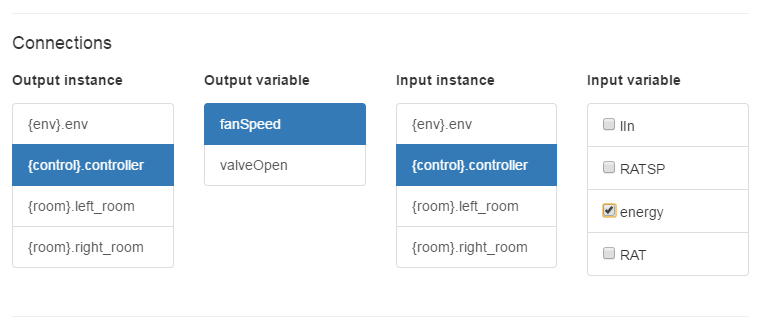
\includegraphics[width=\textwidth]{./figures/app/mm-conns}
\caption{Connections configuration.}
\label{fig:mm-conns}
\end{figure}
%
%
%
The \textit{Initial values of parameters} area, shown in
Figure \ref{fig:mm-params}, allows you to set the initial values of any parameters
defined in the FMUs:
%
%
%
\begin{enumerate}
  \item Click the desired FMU instance in the \textit{Instance Column}.
  \item Select the desired parameter in the \textit{Parameters} dropdown box and click \textit{Add}.
      \item Type the parameter value in the box that appears.
\end{enumerate}
%
%
%
\begin{figure}[ht]
  \centering
  \begin{subfigure}[b]{0.8\textwidth}
    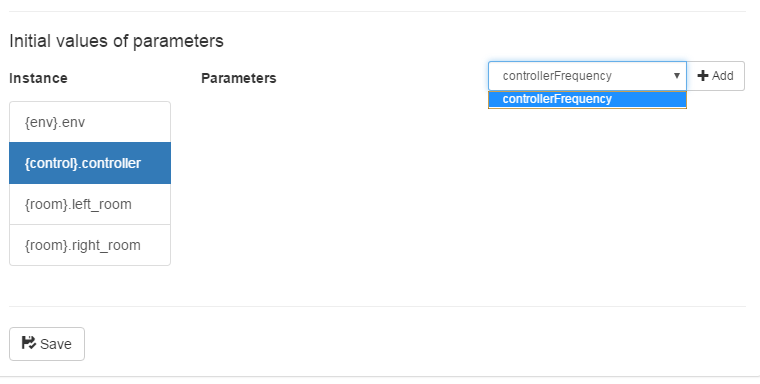
\includegraphics[width=\textwidth]{figures/app/mm-params}
    \caption{Parameter selection.}
    \label{fig:mm-params1}
  \end{subfigure}
  \quad
  \begin{subfigure}[b]{0.8\textwidth}
    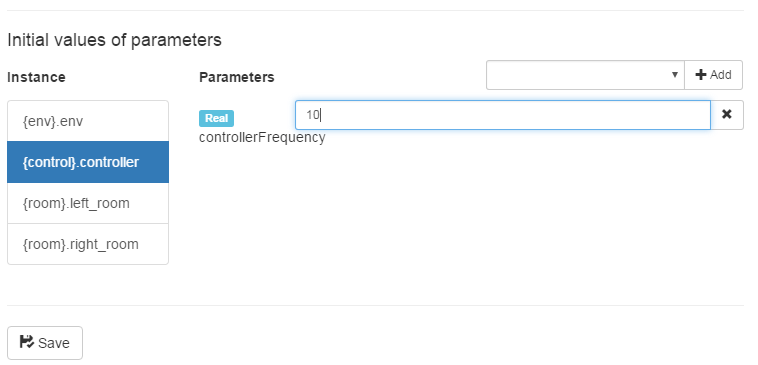
\includegraphics[width=\textwidth]{figures/app/mm-params2}
    \caption{Parameter value input.} 
    \label{fig:mm-params2}
  \end{subfigure}
  \caption{Initial values of parameters configuration.}
  \label{fig:mm-params}
\end{figure}
%
%
%
Once the multi-model configuration is complete, click the \textit{Save}
button at the bottom of the \textit{Configuration} box.
%
\clearpage
%
%
%
\subsection{Co-simulations}
\label{sec:co-simulations}
To execute co-simulations of a multi-model, a co-simulation configuration is
needed. To create a co-simulation configuration, right click the desired
multi-model and select \textit{Create Co-Simulation Configuration}, as shown in Figure \ref{fig:new-cosim}.  After creation, the new configuration automatically opens for editing.
%
%
%
\begin{figure}[ht]
\centering
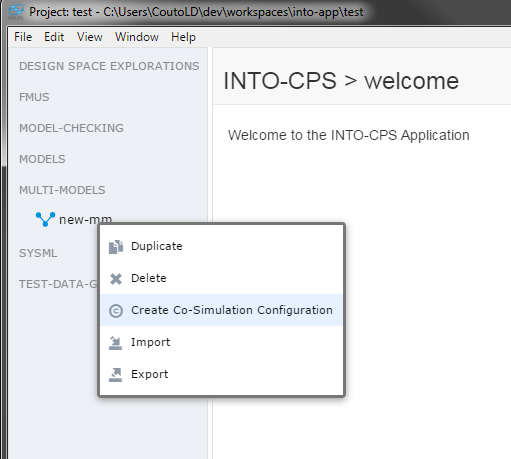
\includegraphics[width=0.7\textwidth]{./figures/app/new-cosim}
\caption{Creating a co-simulation configuration.}
\label{fig:new-cosim}
\end{figure}
%
%
%
To select an existing co-simulation configuration, double-click it. 
Once a configuration is open, the co-simulation configuration, shown in
Figure \ref{fig:cosim-view}, is displayed. The top box, \textit{Configuration},
lets you configure the co-simulation. The bottom box, \textit{Simulation},
lets you execute the co-simulation.
%
%
%
\begin{figure}[ht]
\centering
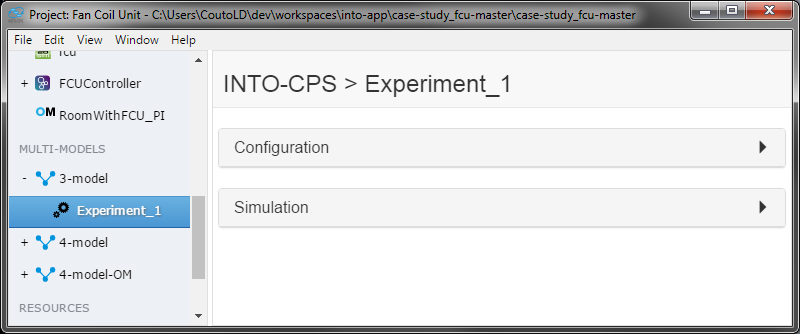
\includegraphics[width=0.8\textwidth]{./figures/app/cosim-view}
\caption{Main co-simulation configuration view.}
\label{fig:cosim-view}
\end{figure}
%
%
%
In order to configure a co-simulation, the configuration must first be unlocked for editing
by clicking the \textit{Edit} button at the bottom of the \textit{Configuration}
box. There are seven things to configure for a co-simulation, discussed next.

\textit{Basic Configuration}, shown in Figure \ref{fig:cosim-top}, allows you to select the start and end time for the co-simulation as well as the master algorithm to be used.
%
%
%
\begin{figure}[ht]
\centering
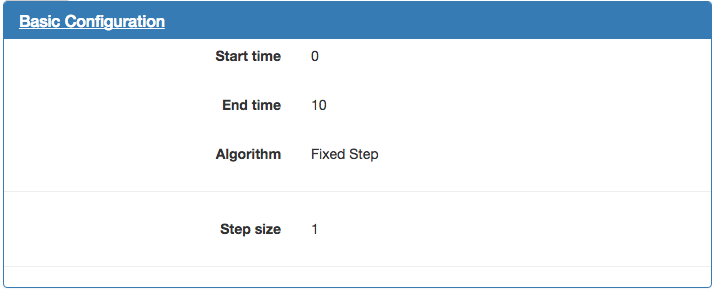
\includegraphics[width=0.8\textwidth]{./figures/app/cosim-top}
\caption{Start/End time and master algorithm configuration.}
\label{fig:cosim-top}
\end{figure}
%
%
%
For every algorithm, there are configuration parameters that can be set. These
are displayed below the top area, as shown in Figure \ref{fig:ma-config}. These parameters differ with the master algorithm chosen.  Parameters are further documented in Deliverable D4.3b \cite{INTOCPSD4.3b}.
%
%
%
\begin{figure}[ht]
\centering
\begin{subfigure}[b]{\textwidth}
  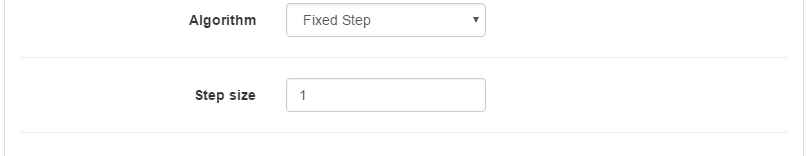
\includegraphics[width=\textwidth]{figures/app/ma-config-fixed}
  \caption{Fixed step size.}
  \label{fig:ma-conf-fix}
\end{subfigure}
\begin{subfigure}[b]{\textwidth}
  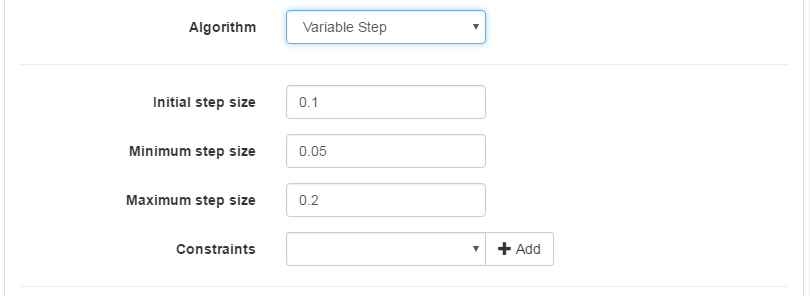
\includegraphics[width=\textwidth]{figures/app/ma-config-variable}
  \caption{Variable step size.}
  \label{fig:ma-conf-var}
\end{subfigure}
\caption{Master algorithm configuration.}
\label{fig:ma-config}
\end{figure}
%
%
%

The \textit{Visibility} area, shown in Figure \ref{fig:visibility-config}, controls loggable FMU output.  \emph{Visible} indicates whether the FMU gives any visible feedback, \emph{e.\@g.\@} graphs.  \emph{Logging on} indicates whether the FMU should use the logging system and send log info back to the COE.  \emph{Enable all log categories per instance} enables all log categories listed inside each FMU.  \emph{Global coe log level override} enables the user to override the pre-set log level in the COE.  This is for debugging failing simulations and should be left unset or at ``error'' or ``warning'' level.
%
%
%
\begin{figure}[ht]
\centering
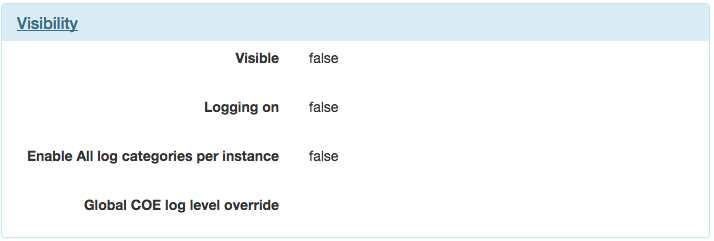
\includegraphics[width=0.9\textwidth]{figures/app/visibility}
\caption{Visibility configuration.}
\label{fig:visibility-config}
\end{figure}
%
%
%

The \emph{Stabilization} area, shown in Figure \ref{fig:stabilization-config}, allows the user to enable the global co-simulation stabilization feature.  These parameters are passed to the NumPy \texttt{isclose()} function\footnote{\url{https://docs.scipy.org/doc/numpy-1.13.0/reference/generated/numpy.isclose.html}}.
%
%
%
\begin{figure}[ht]
\centering
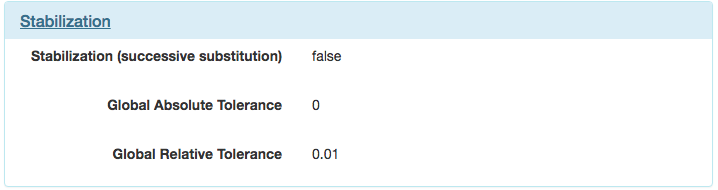
\includegraphics[width=0.9\textwidth]{figures/app/stabilization}
\caption{Stabilization configuration.}
\label{fig:stabilization-config}
\end{figure}
%
%
%

The \textit{Live Plotting} area, shown in Figure \ref{fig:liveplotting-conf}, enables the user to define multiple graphs (currently this comes at a relatively high display cost.)  Each graph can either be external (in its own window) or internal (embedded). The internal graphs are arranged in a configurable grid.  The aim of the grid layout is to eliminate the need for scrolling.  Additional rows are added if no space is left, but these introduce scrolling. When configuring the graphs, it is possible to use a filter on all available scalar variables to find the ones of interest.
%
%
%
\begin{figure}[ht]
\centering
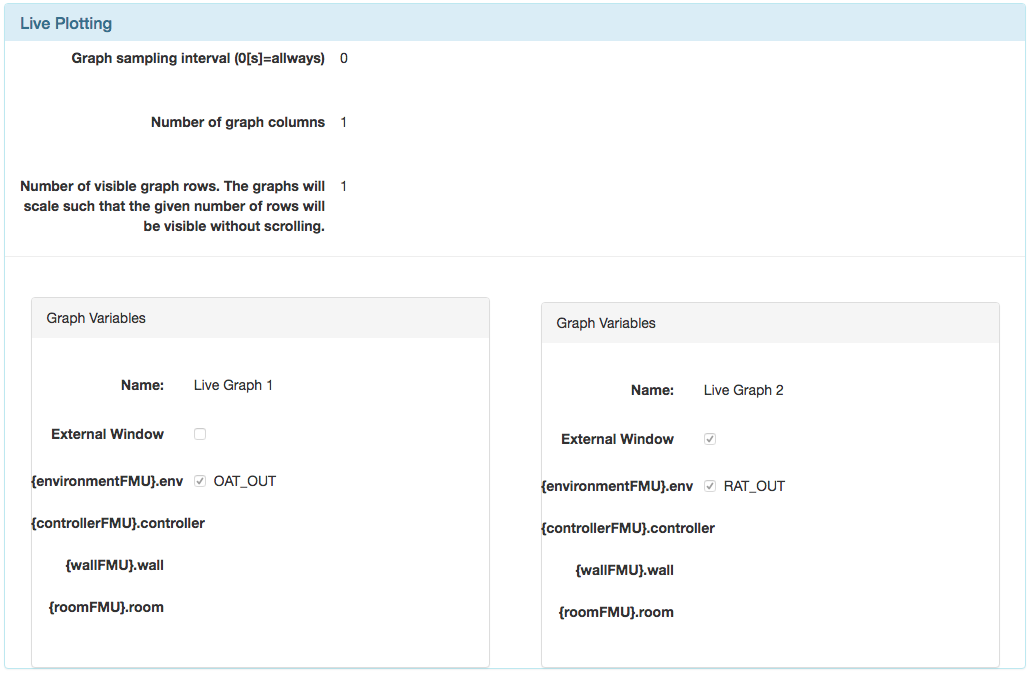
\includegraphics[width=\textwidth]{./figures/app/livePlotting}
\caption{Live plotting configuration.}
\label{fig:liveplotting-conf}
\end{figure}
%
%
%

The \emph{Results Saving} area, shown in Figure \ref{fig:saving-conf}, allows the user to select additional FMU variables to log in the global CSV log file.  All connected variables are logged by default.
%
%
%
\begin{figure}[ht]
\centering
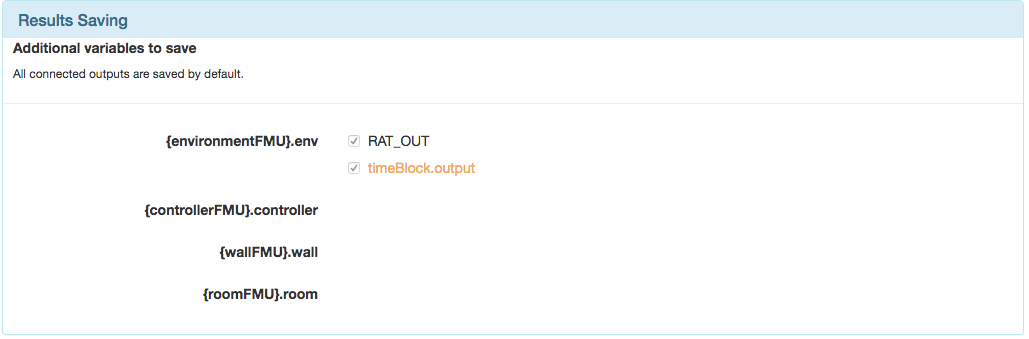
\includegraphics[width=\textwidth]{./figures/app/resultsSaving}
\caption{Results logging configuration.}
\label{fig:saving-conf}
\end{figure}
%
%
%

The \emph{Others} area, shown in Figure \ref{fig:others-conf}, allows the user to slow the co-simulation down to wall time and to enable co-simulation parallelisation.  Please note that parallelising a co-simulation does not always result in a speed-up \cite{Thule&16c}.
%
%
%
\begin{figure}[ht]
\centering
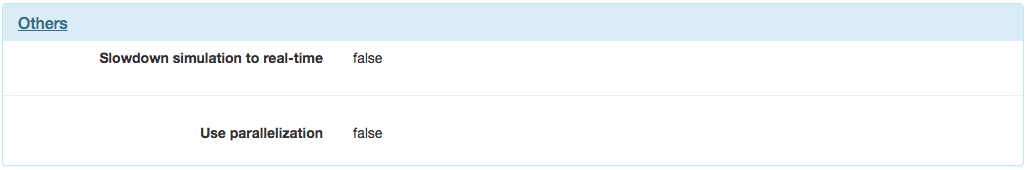
\includegraphics[width=\textwidth]{./figures/app/others}
\caption{Miscellaneous configuration options.}
\label{fig:others-conf}
\end{figure}
%
%
%

The final area, \emph{Post-Processing}, shown in Figure \ref{fig:postprocess}, allows the user to attach a post-processing script written in Python that can be executed at the end of co-simulations.
%
%
%
\begin{figure}[ht]
\centering
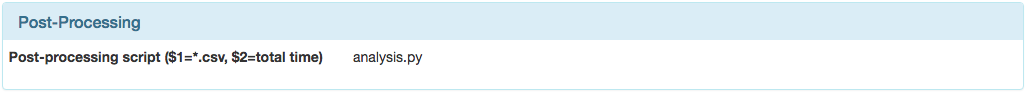
\includegraphics[width=\textwidth]{./figures/app/postProcessing}
\caption{Attaching a post-processing script.}
\label{fig:postprocess}
\end{figure}
%
%
%

Once the co-simulation configuration is complete, click the \textit{Save}
button at the bottom of the \textit{Configuration} box.

The \textit{Simulation} box, shown in Figure \ref{fig:cosim-coe}, allows
you to launch a co-simulation. To run a co-simulation, the COE must be
online. The area at the top of the \textit{Simulation} box displays
the status of the COE. If the COE is offline, you may click the
\textit{Launch} button to start it.
%
%
%
\begin{figure}[ht]
\centering
\begin{subfigure}[b]{0.45\textwidth}
  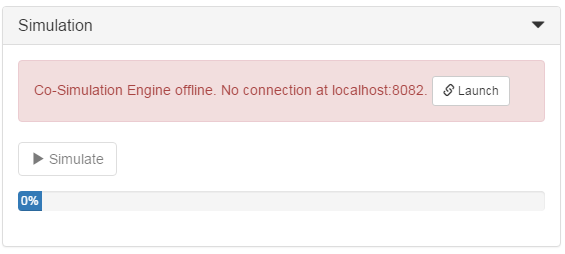
\includegraphics[width=\textwidth]{figures/app/cosim-coe-offline}
  \caption{COE offline.}
  \label{fig:cosim-coe-offline}
\end{subfigure}
\quad 
\begin{subfigure}[b]{0.45\textwidth}
  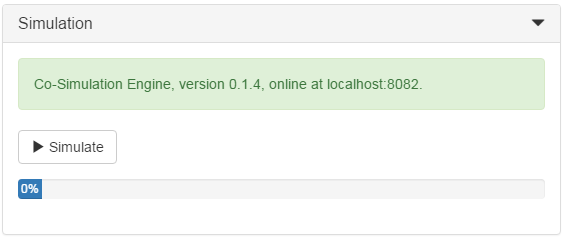
\includegraphics[width=\textwidth]{figures/app/cosim-coe-online}
  \caption{COE online.} 
  \label{fig:cosim-coe-online}
\end{subfigure}
\caption{Launching a co-simulation.}
\label{fig:cosim-coe}
\end{figure}
%
%
%
Once a co-simulation is in progress, any variables chosen for live plotting are plotted in real time in the simulation box, as shown in Figure \ref{fig:cosim-plot}. A progress bar is also displayed.
%
%
%
\begin{figure}[ht]
\centering
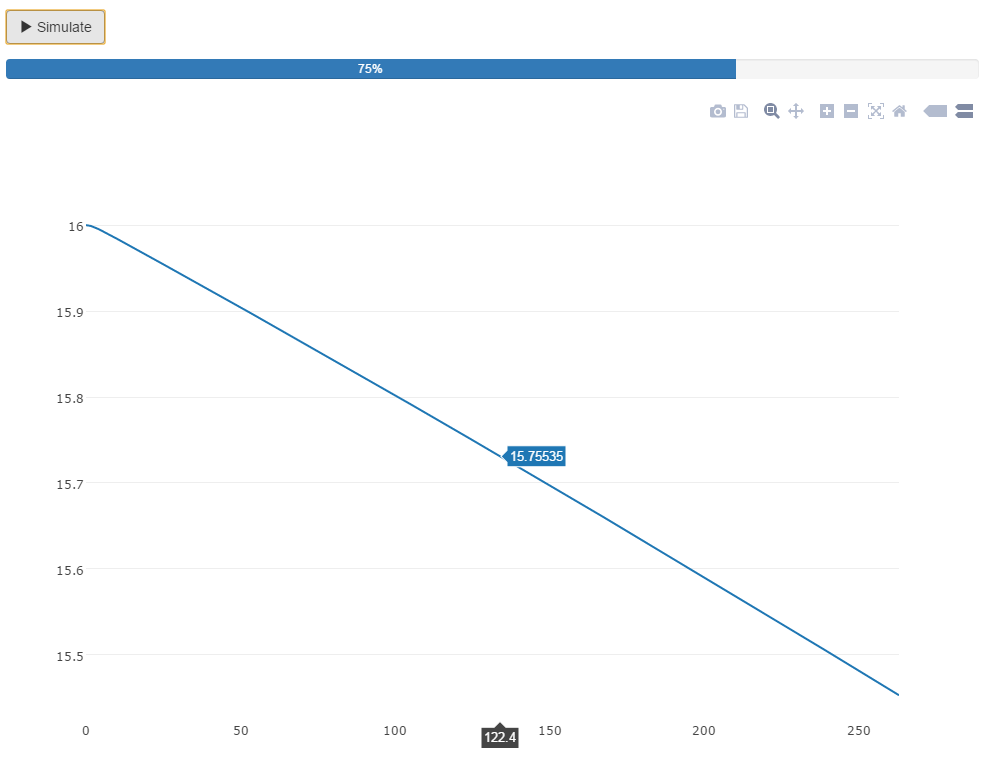
\includegraphics[width=\textwidth]{./figures/app/cosim-plot}
\caption{Live stream variable plot.}
\label{fig:cosim-plot}
\end{figure}
%
%
%
When the simulation is complete, the live stream plot can be explored or
exported as a PNG image. In addition, an \texttt{outputs.csv} file is created
containing the values of every variable marked for logging. This file can be double-clicked and it will open with the
default system program for CSV files. It can also be imported into programs such as R, MATLAB or Excel for more complex analysis. Furthermore, it is possible to add a post-processing script that receives the CSV file name and the total simulation time respectively as arguments. It is also possible to configure the amount of logging performed by the COE.
%
%
%
%\begin{figure}[ht]
%\centering
%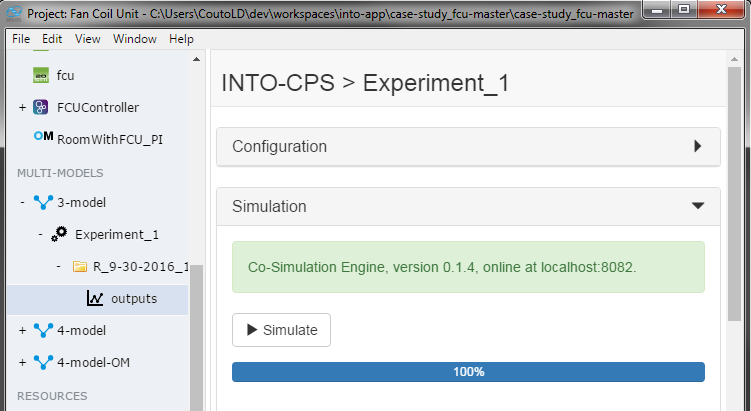
\includegraphics[width=0.85\textwidth]{./figures/app/cosim-results}
%\caption{Co-simulation results file.}
%\label{fig:cosim-results}
%\end{figure}
%
%
%
%\clearpage
%
%
%
\subsection{Additional Features}
\label{sub:other-features}

The \intoapp{} has several secondary features, most of them accessible through
the \textit{Window} menu, as shown in Figure \ref{fig:other-features}. They
are briefly explained below.

\begin{figure}[h!]
\centering
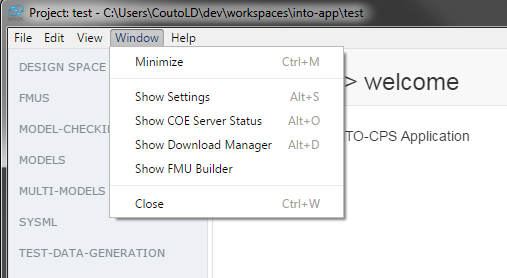
\includegraphics[width=0.65\textwidth]{./figures/app/other-features}
\caption{Additional features.}
\label{fig:other-features}
\end{figure}

\begin{description}
  \item[\texttt{Show Settings}] Displays a settings page where various default
    paths and other options can be set. Development mode can also be enabled from this page, but
    this feature is primarily meant to be used by developers for testing.  Documentation for each setting is found here.
  \item[\texttt{Show Download Manager}] Displays a page where installers can be 
    downloaded for the various tools of the \into tool chain, including the COE.
  \item[\texttt{Show FMU Builder}]  Displays a page that links to a service
    where source code FMUs can be uploaded and cross-compiled for various platforms. Note that this is not a secure service and
    users are discouraged from uploading proprietary FMUs.
\end{description}


\subsection{The Co-Simulation Orchestration Engine}\label{sec:COE}
The heart of the \intoapp{} is the Co-Simulation Orchestration Engine (COE).
%
This is the engine that orchestrates the various simulation tools (described below), carrying out their respective roles in the overall co-simulation.
%
It runs as a stand-alone server hosting the co-simulation API on port 8080.
%
It can be started from the \intoapp{}, but it may be started manually at the command prompt for testing and specialist purposes by executing:
%
%
%
\begin{quote}
\texttt{java -jar coe.jar 8082}
\end{quote}
%
%
%
TCP port 8082 will be chosen by default if it is omitted in the command above.
%
The COE is entirely hidden from the end user of the \intoapp{}, but parts of it are transparently configured through the main interface.
%
The design of the COE is documented in Deliverable D4.1d \cite{INTOCPSD41d}.

The COE is controlled using simple HTTP requests.
%
These are documented in the API manual, which can be obtained directly from the COE by navigating to \url{http://localhost:8082}, once the COE is running.
%
Port 8082 should be changed to that specified when the COE is started.

Following the protocol detailed in the API document, a co-simulation session can be controlled manually from the command prompt using, for example, the \texttt{curl} utility, as demonstrated in the following example.

With the COE running, a session must first be created:
%
%
%
\begin{quote}
\texttt{curl http://localhost:8082/createSession}
\end{quote}
%
%
%
This command will return a \texttt{sessionID} that is used in the following commands.

Next, assuming a COE configuration file called \texttt{coeconf.json} has been created as described in the API manual, the session must be initialized:
%
%
%
\begin{quote}
\texttt{curl -H "Content-Type: application/json" \\ -{}-data @coeconf.json \\ http://localhost:8082/initialize/sessionID}
\end{quote}
%
%
%
Assuming start and end time information has been saved to a file, say \texttt{startend.json}, the co-simulation can now be started:
%
%
%
\begin{quote}
\texttt{curl -H "Content-Type: application/json" \\ -{}-data @startend.json \\ http://localhost:8082/simulate/sessionID}
\end{quote}
%
%
%
Once the co-simulation run ends, the results can be obtained as follows:
%
%
%
\begin{quote}
\texttt{curl -o results.zip \\ http://localhost:8082/result/sessionID/zip}
\end{quote}
%
%
%
The session can now be terminated:
%
%
%
\begin{quote}
\texttt{curl http://localhost:8082/destroy/sessionID}
\end{quote}
%
%
%
The \intoapp{} fundamentally controls the COE in this way.
%
\paragraph{Distributed co-simulations}
Presently the \intoapp{} can only control the COE in this way for non-distributed co-simulations.
%
In order to run a distributed co-si\-mu\-la\-tion, a distributed version of the COE, \texttt{dcoe}, must be controlled from the command prompt manually, as illustrated above.
%
The distributed COE can be downloaded using the App's \emph{Download Manager}.

In a distributed co-simulation the COE and (some) FMUs execute on physically different compute nodes.
%
The FMUs local to the COE computing node are handled in the same way as in standard co-simulations.

Each FMU on the remote nodes is served externally by a daemon process.
%
This process must be started on the remote node manually as follows:
%
%
%
\begin{quote}
\texttt{java -jar daemon*-jar-with-dependencies.jar -host <public-ip> -ip4}
\end{quote}
%
%
%
Here, \texttt{<public-ip>} is the IPv4 address of the compute node.

Next, the distributed COE process must be started manually from the command prompt on its own node, with options specific to distributed co-simulation:
%
%
%
\begin{quote}
\texttt{java -Dcoe.fmu.custom.factory=\\ org.intocps.orchestration.coe.distribution.\\DistributedFmuFactory \\ -jar dcoe*-jar-with-dependencies.jar}
\end{quote}
%
%
%
The second difference is the way in which the location of the remote FMUs is specified.
%
For a standard co-simulation, the \texttt{fmus} clause of the co-simulation configuration file (\texttt{coeconf.json}, in our example) contains elements of the form
%
%
%
\begin{quote}
\texttt{``file://fmu-1-path.fmu''}
\end{quote}
%
%
%
These must be modified for each remote FMU to the following URI scheme:
%
%
%
\begin{quote}
\texttt{``uri://<public-ip>/FMU/\#file://local-fmu-path.fmu''}
\end{quote}
%
%
%
The COE configuration file can, of course, be written manually in its entirety, but it is possible to take a faster route, as follows.

This configuration file is only generated when a co-simulation is executed.
%
It is therefore possible to assemble a ``dummy'' co-simulation that is similar to the desired distributed version, but with a local FMU topology.
%
Since it is likely that the remote FMUs are not supported on the COE platform itself, it is necessary here to construct ``dummy'' FMUs with the same interface.
%
If this local co-simulation is then executed briefly, a COE configuration file will be emitted that can be easily modified as described above.
%
The \intoapp{} will name this file \texttt{config.json} and emit it to the \texttt{Multi-models} folder under each co-simulation run.
%
This modified configuration can then be used to execute the distributed co-simulation.

\clearpage
% !TeX root = ../D4.3a_User_Manual.tex

\section{Modelio and SysML}
\label{sec:SysML}
The INTO-CPS tool chain supports a model-based approach to the development and validation of CPS.
%
The Modelio tool and its SysML/INTO-CPS profile extension provide the diagramming starting point.
%
This section describes the Modelio extension that provides INTO-CPS-specific modelling functionality to the SysML modelling approach.

The INTO-CPS extension module is based on the Modelio SysML extension module, and extends it in order to fulfill INTO-CPS modelling requirements and needs.
%
\autoref{figure:into-cps-example} shows an example of a simple INTO-CPS Architecture Structure Diagram under Modelio.
%
%
%
\begin{figure}[hpt!]
\centering
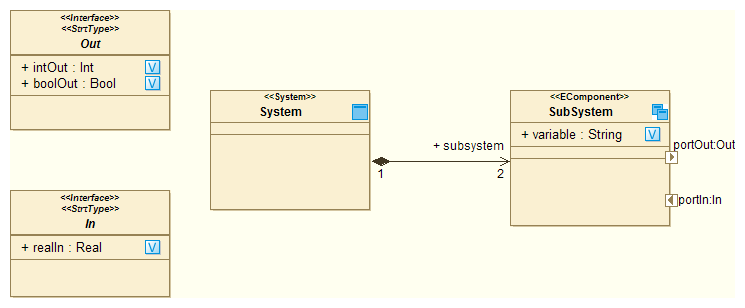
\includegraphics[width=\textwidth]{./figures/modelio-intocps-extension.png}
\caption{Example INTO-CPS multi-model.}
\label{figure:into-cps-example}
\end{figure}
%
%
%
This diagram shows a \textit{System}, named ``System''\footnote{An abstract description of an INTO-CPS multi-model.},  composed of two \textit{EComponent}s of kind \textit{Subsystem}, named ``SubSystem''\footnote{Abstract descriptions of INTO-CPS constituent models.}. These \emph{Subsystem}s have an internal \textit{Variable} called ``variable'' of type \textit{String} and expose two \textit{FlowPort}s named ``portIn'' and ``portOut''. The type of data going through these ports is respectively defined by types \emph{In} and \emph{Out} of kind \textit{StrtType}.
%
More details on the SysML/INTO-CPS profile can be found in Deliverable D2.3a \cite{INTOCPSD2.3a}.

\autoref{figure:sysml-general-aspect} illustrates the main graphical interface after Modelio and the INTO-CPS extension have been installed.
%
%
\begin{figure}[hpt!]
\centering
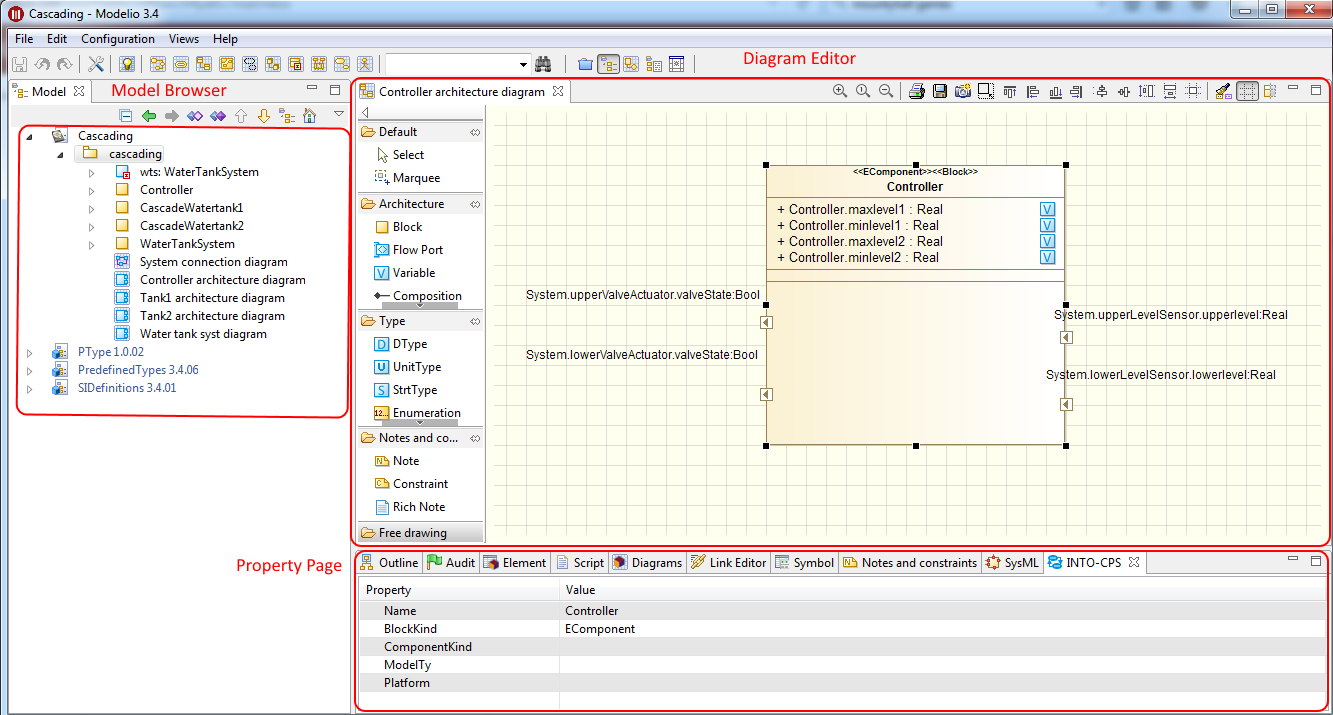
\includegraphics[width=\textwidth]{./figures/sysml-general-aspect.png}
\caption{Modelio for INTO-CPS.}
\label{figure:sysml-general-aspect}
\end{figure}
%
%
Of all the panes, the following three are most useful in the INTO-CPS context.
%
%
%
\begin{enumerate}
\item The Modelio model browser, which lists all the elements of your model in tree form.
\item The diagram editor, which allows you to create INTO-CPS design architectures and connection diagrams.
\item The INTO-CPS property page, in which values for properties of INTO-CPS subsystems are specified.
\end{enumerate}
%
%
%
\subsection{Creating a New Project}
In the INTO-CPS Modelling workflow described in Deliverable D3.3a \cite{INTOCPSD3.3a}, the first step will be to create, as depicted in \autoref{figure:modelio-project-creation}, a Modelio project:

%
\begin{figure}[hpt!]
\centering
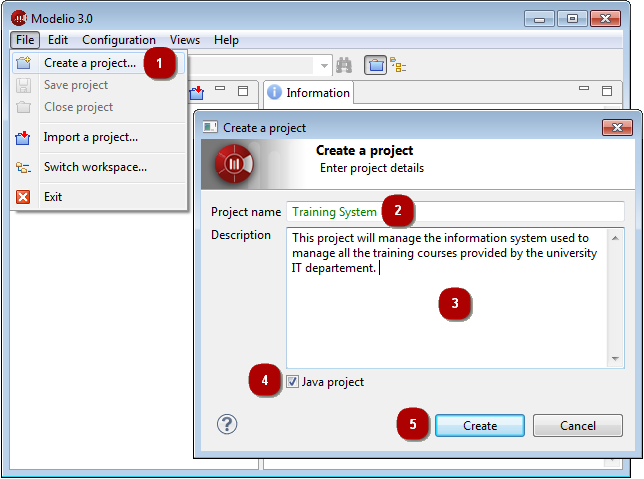
\includegraphics[width=0.8\textwidth]{./figures/modelio-createnewproject.png}
\caption{Creating a new Modelio project.}
\label{figure:modelio-project-creation}
\end{figure}
%
%
%
\begin{enumerate}
\item Launch Modelio.
\item Click on \emph{File} $\rightarrow$ \emph{Create a project...}.
\item Enter the name of the project.
\item Enter the description of the project.
\item If it is envisaged that the project will be connected to a Java development workflow in the future (unrelated to INTO-CPS), you can choose to include the Java Designer module by selecting \emph{Java Project}, otherwise de-select this option.
\item Click on \emph{Create} to create and open the project.
\end{enumerate}
%
%
%
Once you have successfully created a Modelio project, you have to install the Modelio extensions required for INTO-CPS modelling, \emph{i.\@e.\@} both Modelio SysML and INTO-CPS extensions, as described at
%
%
%
\begin{quote}
\url{http://into-cps-association.github.io}
\end{quote}
%
%
%
If both modules have been correctly installed, you should be able to create, under any package, an INTO-CPS Architecture Structure Diagram in order to model the first subsystem of your multi-model.
%
For that, in the Modelio model browser, right click on a \textit{Package} element then in the \textit{INTO-CPS} entry, choose \textit{Architecture Structure Diagram} as shown in \autoref{figure:sysml-create-architecturediagram}.
%
\begin{figure}[hpt!]
\centering
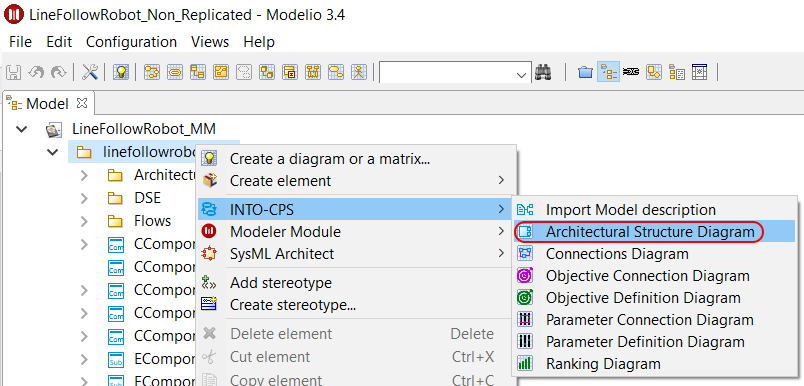
\includegraphics[width=\textwidth]{./figures/sysml-create-architecturediagram.png}
\caption{Creating an Architecture Structure diagram.}
\label{figure:sysml-create-architecturediagram}
\end{figure}
%
Once you are sure that the modules have been correctly installed. You are able to start your INTO-CPS SysML modelling. 
%INTO-CPS Modelling consists in two possible kind of modelling.
%\begin{enumerate}
%  \item In Modelio, right-click on the model block in the tree.
%  \item Select \textit{INTO-CPS} $\rightarrow$ \textit{Generate Model Description} (see \autoref{figure:modelio_export_modelDescription}).
%\end{enumerate}
 
\subsection{INTO-CPS SysML modelling}

INTO-CPS SysML modelling activitIES can be succinctly described as the creation and population of INTO-CPS SysML diagrams.
\autoref{figure:sysml-create-architecturediagram} shows you how to create an Architecture Structure Diagram. 
\autoref{figure:sysml-architecture-diagram} represents an example of an Architecture Structure Diagram.
%
\begin{figure}[hpt!]
\centering
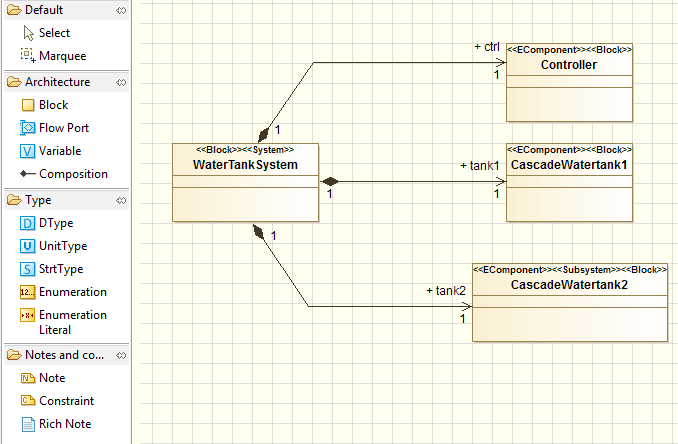
\includegraphics[width=\textwidth]{./figures/sysml-architecture-diagram.png}
\caption{Example Architecture Structure diagram.}
\label{figure:sysml-architecture-diagram}
\end{figure}
%
Besides creating an Architecture Structure Diagram from scratch and specifying by hand the \emph{blocks} of your system, the INTO-CPS extension allows the user to create a block from an existing \texttt{model\allowbreak{}Description\allowbreak{}.xml} file .
%
A \texttt{model\allowbreak{}Description\allowbreak{}.xml} file is an artifact defined in the FMI standard which specifies, in XML format, the public interface of an FMU.
%
To import a \texttt{model\allowbreak{}Description\allowbreak{}.xml} file,
%
%
\begin{enumerate}
\item  Right click in the Modelio model browser on a \textit{Package} element, then in the \textit{INTO-CPS} entry choose \textit{Import Model description}, as shown in \autoref{figure:sysml-reverse}.   
%
\item  Select the desired \texttt{model\allowbreak{}Description\allowbreak{}.xml} file (or the \texttt{.fmu} file that should contain a \texttt{model\allowbreak{}Description\allowbreak{}.xml} file ) in your installation and click on \textit{Import} (\autoref{figure:sysml-reverse-selection}).
\end{enumerate}
%
%
\begin{figure}[hpt!]
\centering
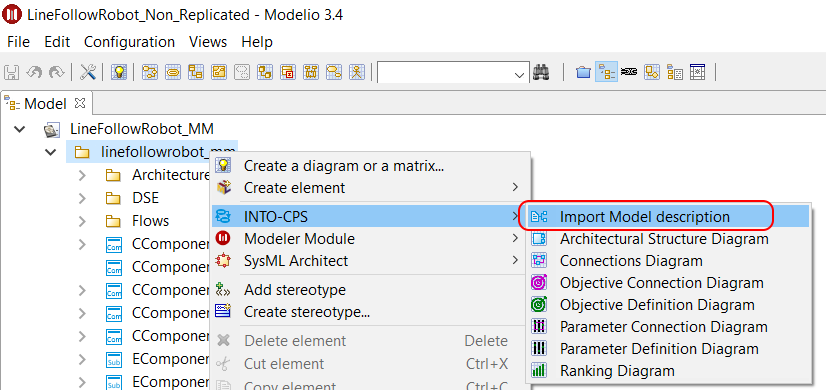
\includegraphics[width=\textwidth]{./figures/sysml-reverse.png}
\caption{Importing an existing model description.}
\label{figure:sysml-reverse}
\end{figure}
%
%
\begin{figure}[hpt!]
\centering
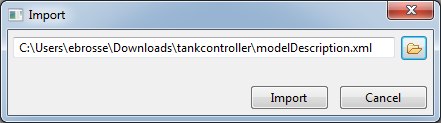
\includegraphics[width=0.7\textwidth]{./figures/sysml-reverse-selection.png}
\caption{Model description selection.}
\label{figure:sysml-reverse-selection}
\end{figure}
%
%
%
This import command creates an Architecture Structure Diagram describing the interface of an INTO-CPS block corresponding to the \texttt{model\allowbreak{}Des\-crip\-tion\allowbreak{}.xml} file imported, \emph{cf.\@} \autoref{figure:sysml-reverse-result}.  
%
%
%
\begin{figure}[hpt!]
\centering
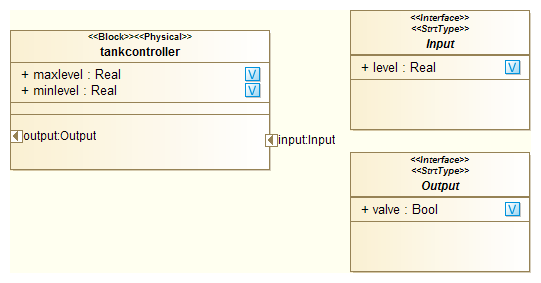
\includegraphics[width=0.8\textwidth]{./figures/sysml-reverse-result.png}
\caption{Result of model description import.}
\label{figure:sysml-reverse-result}
\end{figure}
%
%
%
Once you have created several such blocks, either from scratch or by importing \texttt{model\allowbreak{}Description\allowbreak{}.xml} files, you must eventually connect instances of them in an INTO-CPS Connection Diagram.
%
To create an INTO-CPS Connection diagram, as for an INTO-CPS Architecture Structure Diagram, right click on a \textit{Package} element, then in the \textit{INTO-CPS} entry choose \textit{Connection Diagram}, as shown in \autoref{figure:sysml-create-connectiondiagram}.
%
\autoref{figure:sysml-connectiondiagram-usage} shows the result of creating such a diagram.
%
%
%
\begin{figure}[hpt!]
\centering
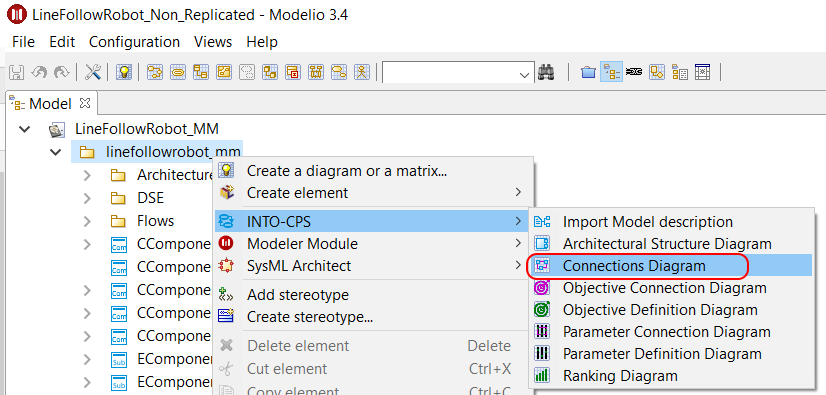
\includegraphics[width=\textwidth]{./figures/sysml-create-connectiondiagram.png}
\caption{Creating a Connection diagram.}
\label{figure:sysml-create-connectiondiagram}
\end{figure}
%
%
%
Once you have created all desired block instances and their ports by using the dedicated command in the Connection Diagram palette, you will be able to model their connections by using the connector creation command (\autoref{figure:sysml-connection-final}).
%
%
%
\begin{figure}[hpt!]
\centering
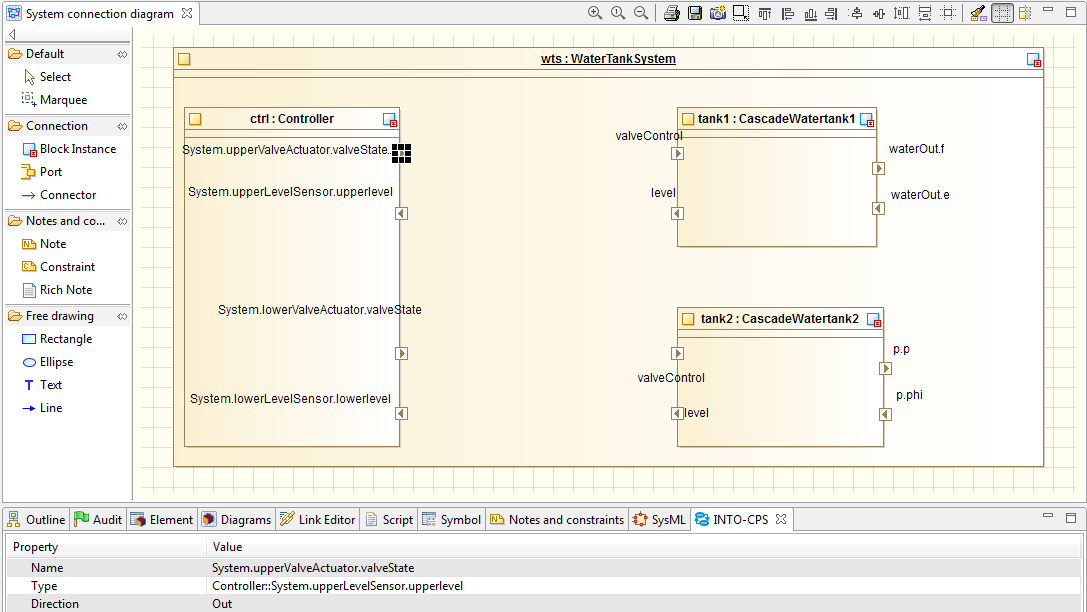
\includegraphics[width=\textwidth]{./figures/sysml-connectiondiagram-usage.png}
\caption{Unpopulated Connection diagram.}
\label{figure:sysml-connectiondiagram-usage}
\end{figure}
%
%
%
\begin{figure}[hpt!]
\centering
\includegraphics[width=\textwidth]{./figures/sysml-connection-final.png}
\caption{Populated Connection diagram.}
\label{figure:sysml-connection-final}
\end{figure}
%
%
%
At this point your blocks have been defined and the connections have been set.
%
The next step is to simulate your multi-model using the INTO-CPS Application.
%
For that you must first generate a configuration file from your Connection diagram.
%
Select the top element in the desired Connection diagram, right click on it and in the \emph{INTO-CPS} entry choose \emph{Generate configuration}, as shown in \autoref{figure:sysml-generateconfig}.
%
%
%
\begin{figure}[hpt!]
\centering
\includegraphics[width=\textwidth]{./figures/sysml-generateconfig.png}
\caption{Generating a configuration file.}
\label{figure:sysml-generateconfig}
\end{figure}
%
%
%
In the final step, choose a relevant name and click on \textit{Generate}.

%\subsection{Exporting \texttt{modelDescription.xml} Files}\label{ch:modelio:sec:export_modeldescription}
The SysML Connection diagram defines the components of the system and their connections.
The internals of these block instances are created in the various modeling tools and exported as FMUs.
The modeling tools Overture, {20-sim} and OpenModelica support importing the interface definition (ports) of the blocks in the Connection diagram by importing a \texttt{modelDescription.xml} file containing the block name and its interface definition.

Follow these steps to export a \texttt{modelDescription.xml} file from Modelio:
%
%
\begin{enumerate}
  \item In Modelio, right-click on the model block in the tree.
  \item Select \textit{INTO-CPS} $\rightarrow$ \textit{Generate Model Description} (see \autoref{figure:modelio_export_modelDescription}).
  \item Choose a file name containing the text ``modelDescription.xml'' and click \textit{Export} (see \autoref{figure:modelio_export_modelDescription_choose_filename}).
\end{enumerate}
%
%
%
\begin{figure}[hpt!]
	\centerline{\includegraphics[width=0.9\textwidth]{figures/modelio_export_modelDescription.png}}
	\caption{Exporting a \texttt{modelDescription.xml} file.}
	\label{figure:modelio_export_modelDescription}
\end{figure}
%
%
%
\begin{figure}[hpt!]
	\centerline{\includegraphics[width=0.8\textwidth]{figures/modelio_export_modelDescription_choose_filename.png}}
	\caption{Naming the model description file.}
	\label{figure:modelio_export_modelDescription_choose_filename}
\end{figure}

\subsection{DSE Modelling}

For design space exploration (DSE) purposes, a DSE model can be constructed in Modelio as well. This modelling is done by specifying mainly a DSE analysis, its parameters, its objectives and a ranking method. 
\autoref{figure:modelio_dse_objective_definition} depicts an example of a DSE objective definition.
%
\begin{figure}[hpt!]
	\centerline{\includegraphics[width=0.5\textwidth]{figures/modelio/dse_objective_definition.png}}
	\caption{DSE Objective definition.}
	\label{figure:modelio_dse_objective_definition}
\end{figure}
%
More details and examples can be found in Deliverable D4.2c \cite{INTOCPSD4.2c}.

Once the DSE model has been created, the DSE analysis can be exported to the INTO-CPS Application. To do so, right-click on \emph{DSE Analysis} in the model tree as depicted in \autoref{figure:modelio_dse_export_command}.   
%
\begin{figure}[hpt!]
	\centerline{\includegraphics[width=0.8\textwidth]{figures/modelio/dse_export_command.png}}
	\caption{DSE Export command.}
	\label{figure:modelio_dse_export_command}
\end{figure}
%
In the final step, choose a relevant name and click on \textit{Export}.
%
%
%
\subsection{Behavioural Modelling}\label{sec:SysML:BehaviouralModelling}
For test generation and/or model-checking analysis, a behavioural model of the system is required. This is usually referred to as {\em test model} in order to indicate its purpose. It is typically not identical to the design model, because it can omit or abstract implementation details.
%
The test model needs to capture all inputs and outputs and describe the system's reactions to inputs by means of one or more deterministic state machine diagram. Timing behaviour should be included by means of timers and timer-guarded transitions.
%
For more details and examples refer to the RTT-MBT Manual~\cite{VSI-mbt-man}.

Once the behavioural model has been specified, the \emph{entire model} must be exported in XMI format. To do so, right-click on the \emph{top package} in the model tree as depicted in \autoref{figure:modelio_xmi_export_command}.   
%
\begin{figure}[hpt!]
	\centerline{\includegraphics[width=0.8\textwidth]{figures/modelio/xmi_export_command.png}}
	\caption{XMI Export command.}
	\label{figure:modelio_xmi_export_command}
\end{figure}
%
Then select the file path by using the XMI export window, as shown in \autoref{figure:modelio_xmi_export_window}. Note that compatibility must be set to "EMG UML 3.0.0" and the file extension to ".xmi".
%
\begin{figure}[hpt!]
	\centerline{\includegraphics[width=0.7\textwidth]{figures/modelio/xmi_export_window.png}}
	\caption{XMI export windows.}
	\label{figure:modelio_xmi_export_window}
\end{figure}


\clearpage
\clearpage
% !TeX root = ../D4.2a_User_Manual.tex
% !TeX spellcheck = en_GB

\section{Using the Separate Modelling and Simulation Tools}\label{sec:simulators}
This section provides a tutorial introduction to the FMI-specific functionality of each of the modelling and simulation tools.
%
This functionality is centered on the role of FMUs for each tool.
%
For more general descriptions of each tool, please refer to Appendix~\ref{appendix:tools}.
%
%
%
\subsection{Overture}
\label{sec:simulators:overture}
% !TeX root = D4.1a_User_Manual.tex
Overture implements export of both tool-wrapper as well as standalone FMUs.
%
It also has the ability to import a \texttt{model\-Description.\allowbreak{}xml} file in order to facilitate creating an FMI-compliant model from scratch.
%
A typical workflow in creating a new FMI-compliant VDM-RT model starts with the import of a \texttt{model\-Description.\allowbreak{}xml} file created using Modelio.
%
This results in a minimal project that can be exported as an FMU.
%
The desired model is then developed in this context.
%
This section discusses the complete workflow.
%
%
%
\subsubsection{Installing the FMI import/export plugin for Overture}
In order to use the FMI integration in Overture it is necessary to install a plugin.
Below is a guide to install the plugin:
\begin{enumerate}
	\item Open Overture.
	\item Select \textit{Help} -> \textit{Install New Software}.
	\item Click \textit{Add..}.
	\item In the \textit{Name:} field write \textit{Overture FMU}.
	\item In the \textit{Location:} field there are two options:
		\begin{description}
			\item[INTO-CPS Application:] Download the \textit{Overture FMU Import / Exporter - Overture FMI Support} using the Download Manager mentioned in Section \ref{sub:other-features}. Locate the file using the \textit{Archive...} button next to the \textit{Location:} field.
			\item[Update site:] Enter the following URL in the \textit{Location:} field: \\ \textit{http://overture.au.dk/into-cps/vdm-tool-wrapper/master/latest}.
		\end{description}
	\item Check the box next to \textit{Overture FMI Integration} as shown in Figure \ref{fig:importFMIoverture}.
	\item Click \textit{Next} or \textit{Finish} to accept and install.
\end{enumerate}
\begin{figure}[ht]
	\centering
	\includegraphics[width=5in]{figures/installOvertureFmiIntegration.png}
	\caption{Installing Overture FMI Integration.}
	\label{fig:importFMIoverture}
\end{figure}
%
%
%
\subsubsection{Import of \texttt{model\-Description.\allowbreak{}xml} File}
A \texttt{model\-Description.\allowbreak{}xml} file is easily imported into an existing, typically blank, VDM-RT project from the project explorer context menu as shown in Figure \ref{fig:moddescimportoverture}.
%
%
%
\begin{figure}[ht]
\centering
\includegraphics[width=3.7in]{figures/modelDescImportOverture.png}
\caption{Importing a \texttt{model\-Description.\allowbreak{}xml} file.}
\label{fig:moddescimportoverture}
\end{figure}
%
%
%
This results in the project being populated with the classes necessary for FMU export:
%
%
%
\begin{itemize}
\item  A VDM-RT \texttt{system} class named ``System'' containing the system definition.  The corresponding ``System'' class for the water tank controller FMU is shown in Listing \ref{lst:wtSystem}.
%
\item  A standard VDM-RT class named ``World''.  This class is conventional and only provides an entry point into the model.  The corresponding ``World'' class for the water tank controller FMU is shown in Listing \ref{lst:wtWorld}.
%
\item  A standard VDM-RT class named ``HardwareInterface''.  This class contains the definition of the input and output ports of the FMU.  Its structure is enforced, and a self-documenting annotation scheme\footnote{The annotation scheme is documented on the INTO-CPS website \url{into-cps-association.github.io} under ``\textit{Constituent Model Development} $\rightarrow$ \textit{Overture} $\rightarrow$ \textit{FMU Import/Export}.} is used such that the ``HardwareInterface'' class may be hand-written.  The corresponding ``HardwareInterface'' class for the water tank controller FMU is shown in Listing \ref{lst:wtHWInterface}.
%
\item  The library file \texttt{Fmi.vdmrt} which defines the hardware interface port types used in ``HardwareInterface''.
\end{itemize}
%
%
%
\begin{figure}[ht]
\begin{vdmrt}
system System

instance variables

-- Hardware interface variable required by FMU Import/Export
public static hwi: HardwareInterface := new HardwareInterface();
    

instance variables

  public levelSensor : LevelSensor;
  public valveActuator : ValveActuator;
  public static controller : [Controller] := nil;

	cpu1 : CPU := new CPU(<FP>, 20);
operations

public System : () ==> System
System () == 
(
	levelSensor := new LevelSensor(hwi.level);
	valveActuator :=  new ValveActuator(hwi.valveState); 
	
	controller := new Controller(levelSensor, valveActuator);

	cpu1.deploy(controller,"Controller");
);

end System
\end{vdmrt}
\caption{``System'' class for water tank controller.}
\label{lst:wtSystem}
\end{figure}
%
%
%
\begin{figure}[ht]
\begin{vdmrt}
class World

operations

public run : () ==> ()
run() ==
 (start(System`controller);
  block();
 );

private block : () ==>()
block() ==
  skip;

sync

  per block => false;

end World
\end{vdmrt}
\caption{``World'' class for water tank controller.}
\label{lst:wtWorld}
\end{figure}
%
%
%
\begin{figure}[ht]
\begin{vdmrt}
class HardwareInterface

values
	-- @ interface: type = parameter, name="minlevel";
	public minlevel : RealPort = new RealPort(1.0);
	-- @ interface: type = parameter, name="maxlevel";
	public maxlevel : RealPort = new RealPort(2.0);

instance variables
	-- @ interface: type = input, name="level";
	public level : RealPort := new RealPort(0.0);

instance variables
	-- @ interface: type = output, name="valve";
	public valveState : BoolPort := new BoolPort(false);

end HardwareInterface
\end{vdmrt}
\caption{``HardwareInterface'' class for water tank controller.}
\label{lst:wtHWInterface}
\end{figure}
\clearpage
%
%
%
The port structure used in the ``HardwareInterface'' class is a simple inheritance structure, with a top-level generic ``Port'', subclassed by ports for specific values:  booleans, reals, integers and strings.
%
The hierarchy is shown in Listing \ref{lst:fmivdmrtFile}.
%
When a model is developed without the benefit of an existing \texttt{model\-Description.\allowbreak{}xml} file, this library file can be added to the project from the project context menu, also under the category ``Overture FMU''.
%
%
%
\begin{figure}[ht]
\begin{vdmrt}
class Port

types
	public String = seq of char;
	public FmiPortType = bool | real | int | String;
 
operations

	public setValue : FmiPortType ==> ()
	setValue(v) == is subclass responsibility;

	public getValue : () ==> FmiPortType
	getValue() == is subclass responsibility;
			
end Port

class IntPort is subclass of Port

instance variables
	value: int:=0;

operations
	public IntPort: int ==> IntPort
	IntPort(v)==setValue(v);

	public setValue : int ==> ()
	setValue(v) ==value :=v;

	public getValue : () ==> int
	getValue() == return value;

end IntPort

class BoolPort is subclass of Port

instance variables
	...
\end{vdmrt}
\caption{Excerpt of ``\texttt{Fmi.vdmrt}'' library file defining FMI interface port hierarchy.}
\label{lst:fmivdmrtFile}
\end{figure}
%
%
%

With all the necessary FMU scaffolding in place, the VDM-RT model can be developed as usual.
%
%
%
\subsubsection{Tool-Wrapper FMU Export}
Models exported as tool-wrapper FMUs require the Overture tool to simulate.
%
Export is implemented such that the VDM interpreter and its FMI interface are included in the exported FMU.
%
Overture tool-wrapper FMUs currently support Win32, Win64, Linux64, Darwin64 and require Java 1.7 to be installed and available in the PATH environment variable.

A tool-wrapper FMU is easily exported from the project context menu as shown in Figure \ref{fig:toolwrapperexportoverture}.
%
The FMU will be placed in the \texttt{generated} folder.
%
%
%
\begin{figure}[ht]
\centering
\includegraphics[width=3.5in]{figures/toolWrapperExportOverture.png}
\caption{Exporting a tool-wrapper FMU.}
\label{fig:toolwrapperexportoverture}
\end{figure}
\clearpage
%
%
%
\subsubsection{Standalone FMU Export}
In contrast to tool-wrapper FMUs, models exported as standalone FMUs do not require Overture in order to simulate.
%
Instead, they are first passed through Overture's C code generator such that a standalone implementation of the model is first obtained.
%
Once compiled, this executable model then replaces the combination of VDM interpreter and model, and the FMU executes natively on the co-simulation platform.
%
Currently Mac OS, Windows and Linux are supported.

The export process consists of two steps.
%
First, a source code FMU is obtained from Overture as shown in Figure \ref{fig:standaloneexportoverture}.
%
Second, the \intoapp{} must be used to upload the resulting FMU to the FMU compilation server using the built-in facility described in Section \ref{sub:other-features}.
%
This is accessed by navigating to \emph{Window} $\rightarrow$ \emph{Show FMU Builder}.

Please note that only some features of VDM-RT are currently supported by the C code generator.
%
This is discussed in more detail in Section \ref{sec:CodeGen}.
%
%
%
\begin{figure}[ht]
\centering
\includegraphics[width=3.5in]{figures/standaloneExportOverture.png}
\caption{Exporting a standalone FMU.}
\label{fig:standaloneexportoverture}
\end{figure}
%
%
%
%\clearpage

%
%
%
\subsection{20-sim}\label{sec:simulators:20sim}
This section explains the FMI and INTO-CPS related features of {20-sim}\footnote{Note that 20-sim is Windows-only. However, it can run fine using Wine \cite{winehq2016} on other platforms. For details on using 20-sim under Wine, contact Controllab.}.
%
We focus on the import of \texttt{model\allowbreak{}Description.\allowbreak{}xml} files, standalone and tool-wrapper FMU export (FMU slave), 3D visualization of FMU operation and an experimental FMU import (FMU master) feature.
%
The complete {20-sim} tool documentation can be found in the {20-sim} Reference Manual \cite{20simReference16a}.

\subsubsection{Import of \texttt{modelDescription.xml} File}\label{sec:simulators:20sim:modeldescriptionimport}
{20-sim} can automatically generate an empty {20-sim} submodel
\footnote{Note that the term ``submodel'' here should not be confused with the INTO-CPS notion of a ``constituent model''.  A submodel here is a part in a graphical 20-sim model.}
from a \texttt{mo\-del\-Description\-.xml} file.
To use the \texttt{modelDescription\allowbreak{}.xml} import, you will need to use the special ``4.6.4-intocps'' version of 20-sim\footnote{You can download the INTO-CPS version of 20-sim using the Download Manager in the INTO-CPS Application.}.
%
A \texttt{mo\-del\-Description\allowbreak{}.xml} file can be imported into {20-sim} by using Windows Explorer to drag the \texttt{model\-Description\allowbreak{}.xml} file onto your {20-sim} model (see \autoref{figure:20-sim_import_modelDescription}).
%
%
%
This creates a new empty submodel with a blue icon that has the same inputs and outputs as defined in the \texttt{modelDescription\allowbreak{}.xml} file.
%
%
%
\begin{figure}[hpt]
	\centerline{\includegraphics[width=\textwidth]{figures/20-sim_import_modelDescription.png}}
	\caption{Import a Model Description in 20-sim.}
	\label{figure:20-sim_import_modelDescription}
\end{figure}
%
%
%
\subsubsection{Tool-wrapper FMU Export}\label{sec:simulators:20sim:toolwrapperfmu}
A tool-wrapper FMU is a communication FMU that opens the original model in the modelling tool and takes care of remotely executing the co-simulation steps inside the modelling tool using some tool-supported communication mechanism.
%
{20-sim} supports co-simulation using the XML-RPC-based DESTECS co-simulation interface \cite{DESTECSD32b}.
%
The generation of a tool-wrapper FMU involves two steps that will be explained below:
\begin{enumerate}
  \item Extend the model with co-simulation inputs, outputs and shared design parameters.
  \item Generate a model-specific tool-wrapper FMU.
\end{enumerate}

The tool-wrapper approach involves communication between the co-si\-mu\-la\-tion engine (COE) and the {20-sim} model through the tool-wrapper FMU.
The {20-sim} model should be extended with certain variables that can be set or read by the COE.
These variables are the co-simulation inputs and outputs.
They can be defined in the model in an equation section called \texttt{externals}:  

\begin{lstlisting}
externals
	real global export mycosimOutput;
	real global import mycosimInput;
\end{lstlisting}

To make it possible to set or read a parameter by the co-simulation engine, it should be marked as \texttt{'shared'}:

\begin{lstlisting}
parameters
	// shared design parameters
	real mycosimParameter ('shared') = 1.0;
\end{lstlisting}

The next step is to generate a tool-wrapper FMU for the prepared model.
This requires at least the ``{4.6.3}-intocps'' version of {20-sim}\footnote{You can download the INTO-CPS version of 20-sim using the Download Manager in the INTO-CPS Application.}.
This version of {20-sim} comes with a Python script that generates a tool-wrapper FMU for the loaded model.

To generate the tool-wrapper FMU:
\begin{enumerate}
  \item Make sure that the tool-wrapper prepared {20-sim} model is saved at a writable location.
  The tool-wrapper FMU will be generated in the same folder as the model.
  \item Open the prepared {20-sim} model in {20-sim}.
  \item In the 20-sim Editor window, open the menu \textit{Tools} and select the menu option \textit{Generate Toolwrapper FMU}.
  \item You can find the generated tool-wrapper FMU as \textit{<modelname>.fmu} in the same folder as your model.

\end{enumerate}

%
%
%
\subsubsection{Standalone FMU Export}\label{sec:simulators:20sim:standalonefmu}
Starting with {20-sim} version 4.6, the tool has a built-in option to generate standalone co-simulation FMUs for both FMI 1.0 and 2.0.

To export a {20-sim} submodel as a standalone FMU, make sure that the part of the model that you want to export as an FMU is contained in a submodel and simulate your model to confirm that it behaves as desired.

Next, follow these steps (see also \autoref{figure:20sim_export_fmu}):
%
%
%
\begin{figure}[hbt]
	\centerline{\includegraphics[width=\textwidth]{figures/20-sim_generate_fmu.png}}
	\caption{Export an FMU from 20-sim.}
	\label{figure:20sim_export_fmu}
\end{figure}
%
%
%
\begin{enumerate}
  \item In the Simulator window, choose from the menu: \textit{Tools}.
  \item Select \textit{Real Time Toolbox}.
  \item Click \textit{C-Code Generation}.
  \item Select the \textit{FMU 2.0 export for 20-sim submodel} target. 
  \item Select the submodel to export as an FMU.
  \item Click OK to generate the FMU. This will pop-up a blue window.
\end{enumerate}
%
%
%
Note that to automatically compile the FMU, you will need the Microsoft Visual C++ 2010, 2013 or 2015 compiler installed (normally included with Microsoft Visual Studio, either Express or Community edition).
%
If {20-sim} can find one of the supported VC++ compilers, it starts the compilation and reports where you can find the newly generated FMU.
%
The {20-sim} FMU export also generates a \textit{Makefile} that allows you to compile the FMU on Windows using Cygwin, MinGW, MinGW64 or on Linux or MacOS X.\\
%
{20-sim} can currently export only a subset of the supported modelling language elements as standalone C-code.
%
Full support for all {20-sim} features is only possible through the tool-wrapper FMU approach (described shortly in Section \ref{sec:simulators:20sim:toolwrapperfmu}).
%
The original goal for the {20-sim} code generator was to export control systems into ANSI-C code to run the control system under a real-time operating system.
%
As a consequence, {20-sim} currently only allows code generation for discrete-time submodels or continuous-time submodels using a fixed-step integration method.
%
Support for variable step size integration methods is not yet included by default in the official {20-sim} 4.6 release, but it is already included in the {20-sim} ``4.6.2-intocps'' release and on GitHub (see below).
%
Other language features that are not supported, (or are only partly supported) for code generation, are:
%
%
%
\begin{itemize}
\item \textbf{Hybrid models:} Models that contain both discrete-\@ and continuous-time sections cannot be generated at once. However, it is possible to export the continuous and discrete blocks separate.
\item \textbf{File I/O:} The 20-sim ``{Table2D}'' block is supported; the ``datafromfile'' block is not yet supported.
\item \textbf{External code:} Calls to external code are not supported. Examples are: \texttt{DLL()}, \texttt{DLLDynamic()} and the MATLAB functions.
\item \textbf{Variable delays:} The \texttt{tdelay()} function is not supported due to the requirement for dynamic memory allocation.
\item \textbf{Event functions:} \texttt{timeevent()}, \texttt{frequencyevent()} statements are ignored in the generated code.
\item \textbf{Fixed-step integration methods:} \textit{Euler}, \textit{Runge-Kutta 2} and \textit{Runge-Kutta 4} are supported.
\item \textbf{Implicit models:} Models that contain unsolved algebraic loops are not supported.
\item \textbf{Variable-step integration methods:} \textit{Vode-Adams} and \textit{Modified Backward Differential Formula} (MeBDF) are available on GitHub (see below for the link).
\end{itemize}

The FMU export feature of {20-sim} is being improved continuously based on feedback from INTO-CPS members and other customers. 
%
To benefit from bug fixes and to try the latest FMU export features like variable step size integration methods (\emph{e.\@g.\@} Vode-Adams and MeBDF), you can download the latest version of the {20-sim} FMU export template from:
%
%
%
\begin{quote}
  \url{https://github.com/controllab/fmi-export-20sim}
\end{quote}
%
%
%
Detailed instructions for the installation of the GitHub version of the {20-sim} FMU export template can be found on this GitHub page.
The GitHub FMU export template can be installed alongside the existing built-in FMU export template.
%
%
%

\subsubsection{FMI 2.0 Import}\label{sec:simulators:20sim:fmuimport}
The ``{4.6.4}-intocps'' version of {20-sim} has an experimental option to import an FMU directly in {20-sim} for co-simulation within {20-sim} itself.
This is useful for quickly testing exported FMUs without the need to set-up a full co-simulation experiment in the INTO-CPS application.
Presently it can only import FMI 1.0 and 2.0 \textit{co-simulation} FMUs can be imported.

The procedure for importing an FMU as {20-sim} submodel is similar to importing a \texttt{modelDescription\allowbreak{}.xml} file.
Follow these steps to import an FMU in {20-sim}:
%
%
%
\begin{enumerate}
  \item Copy/move the FMU to the same folder as your model. This is not required but recommended to prevent embedding hardcoded paths in your model.
  \item Using Windows Explorer, drag the FMU file on your {20-sim} model (see \autoref{figure:20-sim_import_fmu}). 
\end{enumerate}
%
%
%
\begin{figure}[ht]
	\centerline{\includegraphics[width=\textwidth]{figures/20-sim_import_fmu.png}}
	\caption{Importing an FMU in 20-sim.}
	\label{figure:20-sim_import_fmu}
\end{figure}
%
%
%
This creates a new submodel with a blue icon that acts as an FMU wrapper. FMU inputs and outputs are translated into {20-sim} submodel input and output signals.
FMU parameters (scalar variables with causality ``parameter'') are also available in {20-sim}.
This means that you can alter the default values of these FMU parameters in {20-sim}.
The altered FMU parameters are transferred to the FMU during the initialization mode phase of the FMU.


%
%
%
\subsection{20-sim 4C}\label{sec:simulators:20sim4C}
This section describes the features of {20-sim 4C} \cite{20sim4C} \footnote{Note that 20-sim 4C is Windows-only, but it can be executed using Wine \cite{winehq2016} on other platforms.} developed specifically in support of INTO-CPS and FMI.
%
{20-sim 4C} is a rapid prototyping tool that facilitates running C code on hardware to control machines and systems.
%
{20-sim 4C} imports models (as generated C code) from multiple sources (\emph{e.\@g.\@} 20-sim) and runs them on hardware targets such as embedded ARM boards (\emph{e.\@g.\@} Raspberry Pi), PCs running real-time Linux and industrial PLCs.

One of the goals of the \into project is to extend the capabilities of the \into tool chain toward executing part of a co-simulation on real hardware in real-time.
%
This is known as Hardware-in-the-Loop (HiL) simulation.
%
This section explains how the FMI import and export features of {20-sim 4C} can be used to execute source code FMUs on hardware targets in co-simulation under the control of the COE.
%
The complete {20-sim} tool documentation can be found in the {20-sim 4C} Reference Manual \cite{20sim4CManual13a}.
%
All details of the implementation of FMI support in 20-sim 4C can be found in Deliverable D4.3b \cite{INTOCPSD4.3b}.
%
%
%
\subsubsection{Source Code FMU Import}\label{sec:simulators:20sim4C:fmuimport}
To import an FMU in {20-sim 4C}, it must first be converted to a valid {20-sim 4C} project.
%
This is currently done via a command line call at the Windows Command prompt.
%
The command to import a source code FMU in {20-sim 4C} is:
%
%
%
\begin{quote}
\texttt{C:\textbackslash{}Program Files (x86)\textbackslash{}20-sim 4C 2.2\textbackslash{}bin\textbackslash{}\\20simparser.exe newfmuProjectName fmuFilename.fmu}\\
\end{quote}
%
%
%
where \texttt{newfmuProjectName} is the name of a new directory in which {20-sim 4C} will generate the new project.
%
This directory is created as a subdirectory of the current directory.
%
An example is shown in \autoref{figure:20-sim-4C_fmu_import1}.
%
%
%
\begin{figure}[hpt]
	\centerline{\includegraphics[width=\textwidth]{figures/20-sim-4C_fmu_import1.png}}
	\caption{Import a source code FMU in 20-sim 4C.}
	\label{figure:20-sim-4C_fmu_import1}
\end{figure}
%
%
%
This example creates a new directory in \texttt{C:\textbackslash{}Temp\textbackslash{}fmi2} named \texttt{Controller\_TorsionBar} and briefly shows the import dialog from \autoref{figure:20-sim-4C_fmu_import2}.
%
%
%
\begin{figure}[hpt]
	\centerline{\includegraphics[width=0.8\textwidth]{figures/20-sim-4C_fmu_import2.png}}
	\caption{20-sim 4C FMU importer.}
	\label{figure:20-sim-4C_fmu_import2}
\end{figure}
%
%
%
After successfully extracting and importing the FMU, 20-sim 4C will start.

Source code FMUs are deployed to a real-time target as follows:
%
%
%
\begin{enumerate}
\item The 20-sim 4C window (\autoref{figure:20-sim-4C_select_target}) shows the name of the FMU and its public variables and parameters in the tree at the left side.
% 
\begin{figure}[hpt]
	\centerline{\includegraphics[width=\textwidth]{figures/20-sim-4C_select_target.png}}
	\caption{20-sim 4C project with imported FMU.}
	\label{figure:20-sim-4C_select_target}
\end{figure}
%
\item Use the \textit{Select} button in the \textit{Target Template Selection} box to select the hardware target for the FMU.  This shows the \textit{Select Target Configuration} dialog (\autoref{figure:20-sim-4C_select_raspberry_pi}.)
%
\begin{figure}[hpt]
	\centerline{\includegraphics[width=\textwidth]{figures/20-sim-4C_select_raspberry_pi.png}}
	\caption{Select the Raspberry Pi target.}
	\label{figure:20-sim-4C_select_raspberry_pi}
\end{figure}
%
\item Select the \textit{Raspberry Pi 3 (Raspbian, Xenomai 2.6.5)} target.
\item Press the \textit{OK} button to confirm. This will automatically trigger a network scan to find the Raspberry Pi on the network.
\item In case multiple targets are found, select the desired target in the \textit{Please select a target} dialog (\autoref{figure:20-sim-4C_select_multiple_targets}) and press \textit{OK}.
%
%
%
\begin{figure}[hpt]
	\centerline{\includegraphics[width=0.8\textwidth]{figures/20-sim-4C_select_multiple_targets.png}}
	\caption{Select the right target.}
	\label{figure:20-sim-4C_select_multiple_targets}
\end{figure}
%
\item In the main 20-sim 4C window, press \textit{Apply} to confirm the target settings.  20-sim 4C will now try to connect to the Raspberry Pi. When the connection is successful, the \textit{Configure} button will turn green.
  See \autoref{figure:20-sim-4C_connect}.
%
\begin{figure}[hpt]
	\centerline{\includegraphics[width=\textwidth]{figures/20-sim-4C_connect.png}}
	\caption{Accept target settings and go to the connection phase.}
	\label{figure:20-sim-4C_connect}
\end{figure}
%
\item Click the \textit{Connect} button to go to the connection phase. This will show the inputs and outputs of the FMU and 20-sim 4C allows you to connect them to the on-board I/O pins.
%
\item To connect an input or output,  select the signal and press the \textit{Connect} button or double-click the signal (\autoref{figure:20-sim-4C_connect_io}.)  This will show the \textit{Connection} dialog as shown in \autoref{figure:20-sim-4C_connect_select_component}.
%
\begin{figure}[hpt]
	\centerline{\includegraphics[width=\textwidth]{figures/20-sim-4C_connect_io.png}}
	\caption{Select an input or output and press \emph{Connect}.}
	\label{figure:20-sim-4C_connect_io}
\end{figure}
%
\item The connection dialog allows you to select an I/O component (\emph{e.\@g.\@} GPIO for digital I/O or PWM; see \autoref{figure:20-sim-4C_connect_select_component}) and a port within this component (typically a physical pin or connector on the target device; see \autoref{figure:20-sim-4C_connect_select_port}).  Select \textit{OK} to confirm the connection.  The I/O available depends on the selected target device.  The Raspberry Pi 3 provides by default only digital inputs and outputs and 2 PWM outputs.  Extension boards are needed for other I/O.\\
  \textbf{\textit{Note:}}  In case you would like to use an extension board or external I2C or SPI based I/O chip or other I/O, feel free to ask Controllab for options to support this in 20-sim 4C.
%
\begin{figure}[hpt]
	\centerline{\includegraphics[width=0.6\textwidth]{figures/20-sim-4C_connect_select_component.png}}
	\caption{Select a component.}
	\label{figure:20-sim-4C_connect_select_component}
\end{figure}
%
\begin{figure}[hpt]
	\centerline{\includegraphics[width=0.6\textwidth]{figures/20-sim-4C_connect_select_port.png}}
	\caption{Select a port.}
	\label{figure:20-sim-4C_connect_select_port}
\end{figure}
%
\item When you have connected all desired inputs and outputs to the I/O, press the \textit{Apply} button (\autoref{figure:20-sim-4C_connect_apply}.)  The \textit{Connect} button will turn green and 20-sim 4C will extend the FMU source code with additional files to provide support for the Raspberry Pi Xenomai real-time Linux and the Raspberry Pi I/O.\\
%
\textbf{\textit{Note:}} It is not required to connect all inputs and outputs to real I/O.  20-sim 4C will show a warning when some inputs or outputs are not connected.  Unconnected inputs will read a zero (0) value by default.  A special real-time toolwrapper FMU can be generated from 20-sim 4C that will allow you to write to unconnected inputs from a co-simulation experiment (see section \ref{sec:simulators:20sim4C:fmuexport}).  This toolwrapper FMU will also allow you to read all FMU exported variables including all inputs and outputs even when inputs and outputs are connected to the I/O.  This toolwrapper FMU is the basis for INTO-CPS HiL simulation with the Raspberry Pi as the real-time target.
%
\begin{figure}[hpt]
	\centerline{\includegraphics[width=\textwidth]{figures/20-sim-4C_connect_apply.png}}
	\caption{Apply the connections and compile the code.}
	\label{figure:20-sim-4C_connect_apply}
\end{figure}
%
\item Press the orange \textit{Compile} button (\autoref{figure:20-sim-4C_connect_apply}) to go to the \textit{Compile} phase.  This will compile the FMU source code and the additional 20-sim 4C source code into a real-time application.
%
\item When the compilation process is ready and successful, click the orange \textit{Command} button to configure the last task settings before uploading the compiled FMU to the Raspberry Pi (\autoref{figure:20-sim-4C_compile}.)
%
\begin{figure}[hpt]
	\centerline{\includegraphics[width=\textwidth]{figures/20-sim-4C_compile.png}}
	\caption{Compilation phase.}
	\label{figure:20-sim-4C_compile}
\end{figure}
%
\item On the \textit{Configure Run} tab (\autoref{figure:20-sim-4C_run_settings}), you can specify the finish time of the FMU or disable it if it should run forever (until reboot/shutdown).  Ensure that the \textit{Discrete Time Interval} has a step size larger than 0.  This value is used as the time (step size) between two FMU ``doStep'' calls and determines the FMU calculation frequency.  The Raspberry Pi 3 is able to support step sizes as low as 0.00005 (20 kHz), but this depends on the FMU computation load and number of connected I/O pins.
%
\begin{figure}[hpt]
	\centerline{\includegraphics[width=\textwidth]{figures/20-sim-4C_run_settings.png}}
	\caption{Configure task run settings.}
	\label{figure:20-sim-4C_run_settings}
\end{figure}
%
\item Press the \textit{Apply} button to store the run settings.  The \textit{Command} button will turn green.
%
\item Click the \textit{Command} button to upload and start your FMU on the Raspberry Pi.  If everything is configured correctly, the FMU will start and 20-sim 4C will monitor its progress and the current value of the FMU variables.
%
\begin{figure}[hpt]
	\centerline{\includegraphics[width=\textwidth]{figures/20-sim-4C_running.png}}
	\caption{FMU is running.}
	\label{figure:20-sim-4C_running}
\end{figure}
%
\item It is also possible to show selected variables in a monitor plot.  You can enable monitoring of a signal by toggling the dot icon in the \textit{Mon} column to a monitor icon.
%
\item Click the large monitor icon on the button bar to show the monitor plot. An example of the monitor plot with three I/O signals is shown in \autoref{figure:20-sim-4C_monitoring_plot}.
%
\begin{figure}[hpt]
	\centerline{\includegraphics[width=0.7\textwidth]{figures/20-sim-4C_monitoring_plot.png}}
	\caption{Variable monitor.}
	\label{figure:20-sim-4C_monitoring_plot}
\end{figure}  
%  
\end{enumerate}
%
%
%
\subsubsection{Real-time toolwrapper FMU export}\label{sec:simulators:20sim4C:fmuexport}
For HiL simulation with a Raspberry Pi, 20-sim 4C is extended with FMU export functionality.
%
The 20-sim 4C FMU export option generates a real-time toolwrapper FMU for the currently loaded 20-sim 4C project.
%
This FMU can be used in the COE to interface the real-time FMU running on the Raspberry Pi with a standard COE co-simulation experment. 
%
Assuming a running application on the Raspberry Pi, FMU export can be performed as follows:
%
%
%
\begin{enumerate}
\item Co-simulation using a toolwrapper FMU uses the unconnected 20-sim 4C inputs.  Make sure that the desired co-simulation inputs are not connected during the 20-sim 4C \textit{Connect} phase (\autoref{figure:20-sim-4C_connect_apply}).
%
\item Export an FMU using the \textit{FMU Export} menu item.  Make sure that the ``Raspberry Pi 3'' target, or the 20-sim 4C  project (your FMU name,) is selected in the left tree.  This is required so that the FMU exporter can find the right 20-sim 4C project.
%
\item Select \textit{Export FMU} from the \textit{Project} menu item. See \autoref{figure:20-sim-4C_export_toolwrapper_fmu}.
% 
\begin{figure}[hpt]
	\centerline{\includegraphics[width=\textwidth]{figures/20-sim-4C_export_toolwrapper_fmu.png}}
	\caption{Export toolwrapper FMU.}
	\label{figure:20-sim-4C_export_toolwrapper_fmu}
\end{figure}
%
\item A command-line window will be displayed showing status information of the FMU toolwrapper creation process.  See \autoref{figure:20-sim-4C_export_toolwrapper_fmu2}.
%
\begin{figure}[hpt]
	\centerline{\includegraphics[width=\textwidth]{figures/20-sim-4C_export_toolwrapper_fmu2.png}}
	\caption{Toolwrapper FMU status.}
	\label{figure:20-sim-4C_export_toolwrapper_fmu2}
\end{figure}
%
\item This window can be closed after noting the location of the generated FMU.
%
\item The newly created FMU can be used in 32-bit and 64-bit Windows FMI co-simulators like the INTO-CPS COE.  Linux and MacOS X compatible versions are not yet available.
\end{enumerate}

%
%
%
\subsection{OpenModelica}
This section explains the FMI and INTO-CPS related features of OpenModelica.
%
The focus is on import of \texttt{model\allowbreak{}Description.\allowbreak{}xml} files and standalone and tool-wrapper FMU export.
%
%
%
\subsubsection{Import of \texttt{modelDescription.xml} Files}\label{sec:simulators:openmodelica:modeldescriptionimport}
OpenModelica can import \texttt{modelDescription\allowbreak{}.xml} interface files created using Modelio and create Modelica models from them.
%
To use the \texttt{modelDescription\allowbreak{}.xml} import feature, you will need to use OpenModelica nightly-builds versions, as this extension is new.
%
Nightly builds can be obtained through the main INTO-CPS GitHub site:
%
%
%
\begin{quote}
\url{http://into-cps-association.github.io}
\end{quote}
%
%
%

To import a \texttt{modelDescription\allowbreak{}.xml} file in OpenModelica one can use:
\begin{enumerate}
\item The OpenModelica Connection Editor GUI (OMEdit): \emph{FMI} $\rightarrow$ \emph{Import FMI Model Description}.
\item A MOS script, \emph{i.\@e.\@} \texttt{script.mos}, see below.
\end{enumerate}
%
%
%
\begin{lstlisting}[language=modelica]
// start script.mos
// import the FMU modelDescription.xml
importFMUModeldescription("path/to/modelDescription.xml"); getErrorString();
// end script.mos
\end{lstlisting}
%
%
The MOS script can be executed from command line via:
\begin{lstlisting}
// on Linux and Mac OS
> path/to/omc script.mos
// on Windows
> %OPENMODELICAHOME%\bin\omc script.mos
\end{lstlisting}

%
The result is a generated file with a Modelica model containing the inputs and outputs specified in \texttt{modelDescription\allowbreak{}.xml}.  For instance:
%
%
%
\begin{lstlisting}[language=modelica]
model Modelica_Blocks_Math_Gain_cs_FMU "Output the product of a gain value with the input signal"
  Modelica.Blocks.Interfaces.RealInput u  "Input signal connector" annotation(Placement(transformation(extent={{-120,60},{-100,80}})));
  Modelica.Blocks.Interfaces.RealOutput y  "Output signal connector" annotation(Placement(transformation(extent={{100,60},{120,80}})));
end Modelica_Blocks_Math_Gain_cs_FMU;"
\end{lstlisting}
%
%
%
%This functionality will ultimately be integrated in the OMEdit (the OpenModelica Connection Editor) graphical user interface.
%
%
%
\subsubsection{FMU Export}
All FMUs exported from OpenModelica are standalone. There are two ways to export an FMU:
%
%
%
\begin{enumerate}
\item From a command prompt.
\item From OMEdit (OpenModelica Connection Editor).
\end{enumerate}
%
%
%
\paragraph{FMU export from a command prompt}
%
To export an FMU for co-simulation from a Modelica model, a Modelica script file \texttt{generateFMU.mos} containing the following calls to the OMC compiler can be used:
%
%
%
\begin{lstlisting}[language=modelica]
// load Modelica library
loadModel(Modelica); getErrorString();

// load other libraries if needed
// loadModel(OtherLibrary); getErrorString();

// generate the FMU: PathTo.MyModel.fmu
translateModelFMU(PathTo.MyModel, "2.0", "cs"); getErrorString();
\end{lstlisting}
%
%
%
Next, the OMC compiler must be invoked on the \texttt{generateFMU\allowbreak{}.mos} script:
%
%
\begin{lstlisting}
// on Linux and Mac OS
> path/to/omc generateFMU.mos
// on Windows
> %OPENMODELICAHOME%\bin\omc generateFMU.mos
\end{lstlisting}
%
%
%
\paragraph{FMU export from OMEdit}
One can also use OMEdit to export an FMU, as detailed in the figures below.
%
%
%
\begin{itemize}
\item Open OMEdit (see \autoref{figure:OMEdit_1}.)
\item Load the model in OMEdit (see \autoref{figure:OMEdit_2}.)
\item Open the model in OMEdit (see \autoref{figure:OMEdit_3}.)
\item Use the menu to export the FMU (see \autoref{figure:OMEdit_4}.)
\item The FMU is now generated (see \autoref{figure:OMEdit_5}.)
\end{itemize}
%
%
%
\begin{figure}[ht]
	\centerline{\includegraphics[width=12.5cm]{figures/OMEdit_1.png}}
	\caption{Opening OMEdit.}
	\label{figure:OMEdit_1}
\end{figure}
%
%
%
\begin{figure}[ht]
	\centerline{\includegraphics[width=12.5cm]{figures/OMEdit_2.png}}
	\caption{Loading the Modelica model in OMEdit.}
	\label{figure:OMEdit_2}
\end{figure}
%
%
%
\begin{figure}[ht]
	\centerline{\includegraphics[width=12.5cm]{figures/OMEdit_3.png}}
	\caption{Opening the Modelica model in OMEdit.}
	\label{figure:OMEdit_3}
\end{figure}
%
%
%
\begin{figure}[ht]
	\centerline{\includegraphics[width=12.5cm]{figures/OMEdit_4.png}}
	\caption{Exporting the FMU.}
	\label{figure:OMEdit_4}
\end{figure}
%
%
%
\begin{figure}[ht]
	\centerline{\includegraphics[width=12.5cm]{figures/OMEdit_5.png}}
	\caption{Final step of FMU export.}
	\label{figure:OMEdit_5}
\end{figure}
%
%
%
The generated FMU will be saved to \texttt{\%{}TEMP\%{}\textbackslash{}OpenModelica\textbackslash{}OMEdit}.
\clearpage
\subsection{Unity}\label{sec:simulators:unity}
This section describes the 3D visualisation functionality of the \into tool chain.
%
This capability is encapsulated into a Unity-based FMU that is configured and loaded into co-simulations in the usual manner.
%
Unity is a professional game engine.
%
It can be downloaded from the Unity website \cite{UnityWebsite}. 

\subsubsection{Importing the Unity Package into Unity}
To create a 3D animation FMU using Unity, first create a new project or open an existing Unity project. A Unity package was made by CLP that can be imported into Unity to expand Unity with FMU export options. This Unity package can be downloaded via the Download Manager in the INTO-CPS application or by contacting CLP.
%
First, drag-and-drop this package into the \textit{Assets} folder in Unity (in the \textit{Project} tab). See \autoref{figure:20-sim_import_unity_package} on how to import the package from the explorer into Unity. A pop-up will open, like the one shown in \autoref{figure:20-sim_import_unity_package_dialog}. Press the \textit{Import} button, as shown in \autoref{figure:20-sim_import_unity_package_dialog}.
%
\begin{figure}[ht]
	\centerline{\includegraphics[width=0.6\textwidth]{figures/20sim_Unity1.png}}
	\caption{Importing the Unity package into Unity.}
	\label{figure:20-sim_import_unity_package}
\end{figure}
%
\begin{figure}[ht]
	\centerline{\includegraphics[width=0.4\textwidth]{figures/20sim_Unity2.png}}
	\caption{Summary of what will be imported into the Unity project.}
	\label{figure:20-sim_import_unity_package_dialog}
\end{figure}
%
Since the package contains scripts that will modify the Unity editor, it is necessary to restart the Unity project after importing the package. 
%
%
%
\subsubsection{Importing the FMUBuilder \textit{gameobject}}
After restarting Unity, go to the \textit{Hierarchy} tab. Right click within the blank part of the hierarchy (\emph{i.\@e.\@} do not select any objects in the hierarchy) and select \textit{FMU \textrightarrow FMUBuilder} (see \autoref{figure:20-sim_unity_create_fmubuilder}). This will create a new object in the hierarchy named FMUBuilder. When selecting this FMUBuilder object in the hierarchy, a few options will be shown in the \textit{Inspector} (see \autoref{figure:20-sim_unity_components_fmubuilder}). There are three components visible: \textit{Transform}, \textit{FMU Builder (Script)} and \textit{Scenery Conversion (Script)}. The latter two are unique to the INTO-CPS Unity FMU package. \textit{FMU Builder (Script)} is the component that will eventually build the 3D animation FMU, which will be covered later in this section. The other component, \textit{Scenery Conversion (Script)}, is used to convert existing 20-sim sceneries into Unity sceneries. This will also be covered later in this section.

\begin{figure}[ht]
	\centerline{\includegraphics[width=0.5\textwidth]{figures/20sim_Unity3.png}}
	\caption{Creating the FMUBuilder \textit{gameobject} in the hierarchy tab.}
	\label{figure:20-sim_unity_create_fmubuilder}
\end{figure}

\begin{figure}[ht]
	\centerline{\includegraphics[width=0.7\textwidth]{figures/20sim_Unity4.png}}
	\caption{Components of the FMUBuilder in the \emph{Inspector} tab in Unity.}
	\label{figure:20-sim_unity_components_fmubuilder}
\end{figure}

\subsubsection{Assigning FMU Variables to Unity \textit{gameobject}s}
To be able to connect variables from a co-simulation to an object in Unity, a \textit{gameobject} is needed. For example, as shown in \autoref{figure:20-sim_unity_create_fmubuilder}, a cube object can be created by right-clicking in the hierarchy tab in a blank space of the hierarchy, but now selecting \textit{3D Object \textrightarrow Cube}.
%
When the newly created object is selected in the hierarchy, all components currently attached to this cube can be seen in the \textit{Inspector} tab.
%
At the bottom of this tab there is a button named \textit{Add Component}. Press this button, go to \textit{FMU variables} and choose between \textit{20-sim coordinates} or \textit{Unity coordinates}.
%
The first one means that the axes are part of a right-handed frame, that the Z-axis is pointing up, and that the order of rotation for Euler angles is X-Y-Z.
%
The latter is the Unity convention, in which the frame is left-handed, the Y-axis is pointing up, and the rotation for Euler angles is Z-X-Y.
%
See \autoref{figure:20-sim_unity_add_variable} on how to do this.
%
If there is doubt about which of the two types of variables should be chosen, choose the 20-sim option, as this is the reference frame used in most modeling tools like 20-sim.
%
Once one is selected, two additional scripts become available in the \textit{Inspector} tab. These are \textit{GUID (Script)} and either \textit{Twenty Sim Variable (Script)} or \textit{Unity Variable (Script)}. The \textit{GUID} script should not be touched. The \textit{Variable} script, however, is the script that will describe the interface variables of the to-be-generated FMU. Choose an FMU variable name and an axis, and press the \textit{Add Axis} button. Multiple axes can be defined for one \textit{gameobject}. \autoref{figure:20-sim_unity_modify_variable} shows the axes dropdown menu and the \textit{Twenty Sim Variable (Script)} and \textit{GUID (Script)} components. 

\begin{figure}[ht]
	\centerline{\includegraphics[width=0.4\textwidth]{figures/20sim_Unity5.png}}
	\caption{Adding new FMU variables to the Unity scene.}
	\label{figure:20-sim_unity_add_variable}
\end{figure}

\begin{figure}[ht]
	\centerline{\includegraphics[width=0.7\textwidth]{figures/20sim_Unity6.png}}
	\caption{Adding the variable named "DemoVariable" for the x-position axis to the newly generated cube object.}
	\label{figure:20-sim_unity_modify_variable}
\end{figure}

\subsubsection{Converting a 20-sim Scenery into a Unity Scenery}
If a 20-sim scenery already exists, then it is possible to import it into Unity. If there is a 3D animation window in the 20-sim model, then double click the plot to open the \textit{3D Properties} window. Then go to \textit{File \textrightarrow Save Scene} (see \autoref{figure:20-sim_unity_export_scene}). If 20-sim asks to save the whole scenery, select \textit{Yes}. Remember where the scenery file is located and go back to Unity. Go to the hierarchy tab, select \textit{FMUBuilder} and enter under the \textit{Scene Conversion (Script)} the location of the scenery file, by pressing \textit{Find scenery}. Afterwards, press the \textit{Build scenery} button and the 20-sim scene will be loaded underneath the \textit{FMUBuilder} object in the hierarchy (this can be drag-dropped to other places in the hierarchy if needed), see \autoref{figure:20-sim_unity_import_scene} for the hierarchy that is created. Note that the Cube seen in \autoref{figure:20-sim_unity_export_scene} in the hierarchy is now created in Unity as well. Furthermore, the \textit{Default Lights and Cameras} frame is converted into Unity, which is a default set of lights and cameras in every 20-sim 3D scene. 
%
\begin{figure}[ht]
	\centerline{\includegraphics[width=0.7\textwidth]{figures/20sim_Unity7.png}}
	\caption{Exporting a 20-sim 3D scenery from a 3D animation plot.}
	\label{figure:20-sim_unity_export_scene}
\end{figure}
%
\begin{figure}[ht]
	\centerline{\includegraphics[width=0.3\textwidth]{figures/20sim_Unity8.png}}
	\caption{Importing a 20-sim scenery file into Unity.}
	\label{figure:20-sim_unity_import_scene}
\end{figure}
%\clearpage
%
\subsubsection{Exporting an FMU} \label{sec:simulators:20sim:fmuexport}
The final step in the process of creating a 3D animation FMU in Unity is the build process itself. The variables that were added by manually assigning FMU variables to \textit{gameobject}s and by importing 20-sim scenery files will now be used to generate the FMU itself. Every variable name (either the ones manually entered, or automatically generated by the import 20-sim scenery option) will be the input variables of this FMU. Select the \textit{FMUBuilder} in the hierarchy and go to the \textit{Inspector} tab. Under \textit{FMU Builder (Script)} select the export location and the name of the to-be-exported FMU, then press \textit{Build FMU}. Once the build process is done, the FMU will be present in the export location selected, with the given name. Note that for larger Unity scenes this can take a while to build.

\clearpage
\clearpage
\newcommand*{\DSEIcon}{\includegraphics[height=0.8em]{figures/dse/DSEIcon}}%
\newcommand*{\ResultsIcon}{\includegraphics[height=0.8em]{figures/dse/results-actualIcon}}%
%
%
%
\section{Design Space Exploration}\label{sec:DSE}
This section provides a description of \into tool chain support for design space exploration (DSE.)
%
%
This section is split into four parts.  In Section~\ref{sec:dse:install} the installation procedure is outlined. Section~\ref{sec:dse:launch} describes how the \intoapp{} can be used to launch a DSE using an existing configuration file and Section~\ref{sec:dse:results} describes how the results from DSE are generated and stored.  Section~\ref{sec:dse:edit} describes the structure of the DSE configuration file, giving enough detail for the user to be able to edit one for their purposes.
%
%
%
\subsection{Installing DSE Scripts}\label{sec:dse:install}
Before we launch a  DSE, we must install the DSE scripts for the various search algorithms and objective evaluation. In the  \intoapp{}, select  \textit{Window} $\rightarrow$ \textit{Show Download Manager}. This opens the download manager as shown in Figure~\ref{fig:dse:download_mngr}. Select the most recent release and download \textit{Design Space Exploration - Scripts for generating and analysing multiple co-simulations}.
%
Python version 2.7 must be installed, along with the matplotlib library.

\begin{figure}[ht]
	\centering
	\includegraphics[width=0.7\textwidth]{figures/dse/download_mngr}
	\caption{Download Manager.}\label{fig:dse:download_mngr}
\end{figure}

This will download a Zip archive -- extract this into the directory in which the archive was downloaded. DSEs may now be launched.

\subsection{How to Launch a DSE}\label{sec:dse:launch}
To launch a DSE we need to provide the \intoapp{} with the path to two files.  The first is the DSE configuration, defining the parameters of the design space, how it should be searched, measured and the results compared.   The second is the multi-model configuration, defining the base model that will be used for the search.  A DSE configuration is selected by double clicking on one of the configurations listed in the \emph{DSES} section of the \intoapp{} project explorer; these configurations are identified with the (\DSEIcon) icon.  Hint: several of the downloadable examples have predefined  DSE configurations.

To launch the DSE, we must first select the multi-model to use. One can be selected by clicking the \emph{Set multi-model} button and selecting one from the drop-down list, as shown in Figures \ref{fig:dse:launch:selectmultimodel} and \ref{fig:dse:launch:setmultimodel}.  Once selected, your choice must be saved to parse the DSE configuration with respect to the multi-model of choice by clicking on the \emph{Save multi-model choice} button, as shown in Figure~\ref{fig:dse:launch:setmultimodel}.
%
%
%
\begin{figure}
	\centering
	\includegraphics[width=0.8\textwidth]{figures/dse/launch-selectmultimodel}
	\caption{Selecting a multi-model.}\label{fig:dse:launch:selectmultimodel}
\end{figure}

\begin{figure}
	\centering
	\includegraphics[width=0.8\textwidth]{figures/dse/launch-setmultimodel}
	\caption{Setting a multi-model.}\label{fig:dse:launch:setmultimodel}
\end{figure}

If the COE is not already running, the bottom of the DSE page is shown with a red ``\emph{Co-Simulation Engine offline. No connection at localhost:8082}'' status, as shown in Figure \ref{fig:dse:launch:dsesection}.
%
If this is the case, click on the \emph{Launch} button to start the COE.
%
This results in a green co-simulation engine status (see Figure \ref{fig:dse:launch:coerunning}). Pressing the \emph{Simulate} button starts the DSE background process.
%
%
%
\begin{figure}[ht]
	\centering
	\includegraphics[width=0.9\textwidth]{figures/dse/launch-dsesection}
	\caption{Status when COE is not running.}\label{fig:dse:launch:dsesection}
\end{figure}
%
%
%
\begin{figure}[ht]
	\centering
	\includegraphics[width=0.8\textwidth]{figures/dse/launch-coerunning}
	\caption{Status when COE is running.}\label{fig:dse:launch:coerunning}
\end{figure}
%
%
%
%With the DSE configuration selected and the COE running, the next step is to select the multi-model to use.
%
%One can be selected from the \emph{Co-simulation Configuration} drop-down box, as shown in Figure \ref{fig:dse:launch:selectmultimodel}.  Pressing the \emph{Simulate} button starts the DSE background process.
%
%
%
\subsection{Results of a DSE}\label{sec:dse:results}
The DSE scripts store their results in a folder named for the date and time at which the DSE was started.
%
This folder may be found underneath the name of the DSE script selected, as shown in Figure~\ref{fig:dse:results:icon}.  When the DSE has finished, we can find both a graphs folder and an HTML results page inside the results folder.
%
It may be necessary to refresh the project view to see these new items.  The results HTML file is identified by the (\ResultsIcon) icon, and double clicking on it opens the results page in the computer's default browser.
%
%
%
\begin{figure}[ht]
	\centering
	\includegraphics[width=0.8\textwidth]{figures/dse/results-icon}
	\caption{Icon shown when DSE results are ready.}\label{fig:dse:results:icon}
\end{figure}
%
%
%

The results, shown in Figure~\ref{fig:dse:results:page}, contain two elements.  The first element is a Pareto graph showing the results of all simulations on a single plot, with each point on the graph representing a single simulation.  The best designs, referred to as the non-dominated set, are shown in blue, with ranks of progressively worse designs coloured alternately red and yellow.  The second element is a table of these results, with the rank in the left hand column, followed by the objective values and finally the design parameters that produced the result.
%
%
%
\begin{figure}[ht]
	\centering
	\includegraphics[width=\textwidth]{figures/dse/results-page}
	\caption{A page of DSE results.}\label{fig:dse:results:page}
\end{figure}
%
%
%
\subsection{How to Edit a DSE Configuration}\label{sec:dse:edit}

A DSE configuration comprises several elements. In Section~\ref{sec:dse:overview} we outline the content of each element and their role in a DSE. 
There are three methods for producing DSE configurations; through the use of the INTO-SysML DSE profile (Section~\ref{sec:dse:edit:sysml}), through the \intoapp{} (this method may also be used to edit an existing configuration) (Section~\ref{sec:dse:edit:app}), or manually editing a text configuration document (Section~\ref{sec:dse:edit:manual}). In this section we outline each approach.  



\subsubsection{DSE Configuration Overview}\label{sec:dse:overview}

A DSE configuration comprises several elements: the search algorithm to use; parameters; parameter constraints; objectives; objective constraints; a ranking; and a set of scenarios.


\subsubsection*{Search Algorithm}\label{sec:dse:overview:algorithm}

The algorithm section allows a user to choose between DSE search algorithms implemented in INTO-CPS. There are two options at present: \textit{exhaustive} and \textit{genetic}. The exhaustive approach will simulate the whole design space as dictated by the choice of parameters and scenarios. The genetic algorithm uses an approach to selecting the designs to simulate based upon genetic breeding and mutations. For more information on the search algorithms, see Deliverable D3.2a~\cite{INTOCPSD3.2a}.

\subsubsection*{Parameters}\label{sec:dse:overview:parameters}

The parameters section is used to define a list of values for each parameter to be explored.   If a parameter is included in the DSE configuration file, then it must have at least one value defined.  The order of the values in the list is not important. 

\subsubsection*{Parameter Constraints}\label{sec:dse:overview:parameterconstraints}
It may be the case that not all combinations of the parameter values defined in the previous section are valid.
%
So, it is necessary to be able to define constraints over the design parameters such that no time is wasted simulating invalid designs.  For example, in the Line Follower Robot project \cite{INTOCPSD3.6} we define ranges for the x and y co-ordinates of the left and right sensors separately, and running all combinations of these leads to asymmetric designs that do not have the same turning behaviour on left and right turns.  To prevent this we can define boolean expressions based upon the design parameters and evaluate these before a simulation is launched.

\subsubsection*{Objective Definitions: Internal}\label{sec:dse:overview:objectivesinternal}
There are two means for defining the objectives used to assess the performance of a simulated model.  The first of these, described here, is using the internal functions included in the DSE scripts.  This is a set of simple functions that can be applied to any of the values recorded by the COE during simulation.  The current set of internal functions is:
%
%
%
\begin{description}
	\item[max] Returns the maximum value of a variable during a simulation.
	\item[min] Returns the minimum value of a variable during a simulation.
	\item[mean] Returns the mean value of a variable during a simulation (\emph{n.\@b.\@}, a fixed simulation step size is assumed.)
\end{description}
%
%

\subsubsection*{Objective Definitions: External Scripts}\label{sec:dse:overview:objectivesexternal}

The second form of objective definition makes use of user-defined Python scripts to allow bespoke analysis of simulation results to be launched automatically and results recorded using the common format.  The definition has two parts: the construction of the Python script to perform the analysis and the definition of the script's required parameters in the DSE configuration file.  These two steps are described below.

\paragraph{Construction of the Script}

The outline functionality of an analysis script is that, at the appropriate times, a DSE script calls it, passing four or more arguments.  The script uses these arguments to locate a raw simulation results file (\texttt{results.csv}), process those results and then write the objective values into an objectives file (\texttt{objectives.json}) for that simulation.  

The first three arguments sent to the script are common to all scripts.  These are listed below.
%
%
%
\begin{description}
	\item[argv 1 ] The absolute path to the folder containing the \texttt{results.csv} results file.  This is also the path where the script finds the \newline \texttt{objectives.json} file.
	\item[argv 2 ] The name of the objective.  This is the key against which the script should save its results in the objectives file.
	\item[argv 3 ] The name of the scenario.
\end{description}
%
%
%
With this information the script can find the raw simulation data and also determine where to save its results.  The name of the scenario allows the script to locate any data files it needs relating to the scenario.  For example, in the case of the script measuring cross track error for the line following robot, the script makes use of a data file that contains a series of coordinates that represent the line to be followed.  The name of this data file is \texttt{map1px.csv}.  It is placed into a folder with the same name as the scenario, which in this case is \texttt{student\-Map}.  That folder is located in the \texttt{user\-Metric\-Scripts} folder, as shown in Figure~\ref{fig:dse:externalAnalysisDataLocation}.  Using this method, the developer of an external analysis script needs only to define the name of the data file they will need and know that at runtime the script will be passed a path to a folder containing the data file suitable for the scenario under test.
%
%
%
\begin{figure}[ht]
	\centering
	\includegraphics[width=\textwidth]{figures/dse/externalAnalysisDataLocation}
	\caption{External analysis script data files for the ``studentMap'' scenario.}\label{fig:dse:externalAnalysisDataLocation}
\end{figure}

\begin{figure}
	\centering
	\includegraphics[scale=0.55]{figures/dse/cumulativeDeviationWholeScript}
	\caption{External analysis script to calculate cumulative deviation in the Water Tank example.}\label{fig:dse:edit:cumulativeDeviationWholeScript}
\end{figure}


Figure~\ref{fig:dse:edit:cumulativeDeviationWholeScript} shows an example of an external analysis script.  In this case it computes the cumulative deviation of the water level from some target level.  There are two distinct sections in the file, we shall refer to them as the ``common'' and ``script specific'' sections.  

The common section contains core functions that are common to all external scripts.  It reads in the three arguments that are common to all scripts, and contains functions to help the user retrieve the data needed by the analysis script, and to write the computed objective value into the \texttt{objectives.json} file.  It is recommended that this section be copied to form the basis of any new external analysis scripts.

The second part of the example script shown is specific to the analysis to be performed.  The purpose of this section is to actually compute the value of the objective from the results of a simulation.  Generally it will have three parts: reading in any analysis specific arguments such as the ID of data in the results that it needs, using the data in \texttt{results.csv} to calculate the value of the objective and finally write the objective value into \texttt{objectives.json}.

In the `Script Specific Section' of Figure~\ref{fig:dse:edit:cumulativeDeviationWholeScript} we see the example of the script calculating the cumulative deviation of the water level from a target level in the water tank model.  It starts by reading a further two arguments passed when the script is launched and initializes the variables.  The script then iterates through all rows of data in \texttt{results.csv} to calculate the cumulative deviation which is then written to the \texttt{objectives.json} file in the final line.
%
%
%
\subsubsection*{Ranking}\label{sec:dse:overview:ranking}
The final part of a DSE configuration file concerns the placing of designs in a partial order according to their performance.  The DSE currently supports a Pareto method of ranking, as was shown earlier in Figure~\ref{fig:dse:results:page}.  The purpose of the ranking section of the configuration is to define the pair of objectives that will be used to rank the designs, and whether to maximise or minimise each.  

\subsubsection*{Scenario List}\label{sec:dse:overview:scenarios}
The DSE scripts currently have limited support for scenarios referring to a specific set of conditions against which the multi-model is to be tested.  In the example of the line following robot, the scenario refers to the map the robot has to follow, along with its starting co-ordinates.
%
For instance, in one scenario the robot would go around a circular track in one direction, predominantly turning left, whereas in a different scenario the same track would be followed in the opposite direction, predominantly turning right.
%
In both scenarios the map of the track is the same.


%
%
%


\subsubsection{Using the INTO-SysML DSE Profile}\label{sec:dse:edit:sysml}


The INTO-CPS DSE SysML profile is defined in Deliverable D4.2c~\cite{INTOCPSD4.2c}, with an example of its use in Deliverable D3.3a~\cite{INTOCPSD3.3a}. Here we describe the steps to export the configuration from Modelio and import it into the \intoapp{}.

Given a complete DSE SysML model, as shown in Figure~\ref{fig:dse:edit:sysml}, we generate a DSE configuration by right-clicking on the \texttt{DSEAnalysis} object in the model browser and selecting \textit{INTO-CPS} $\rightarrow$ \textit{GenerateDSE}, as in Figure~\ref{fig:dse:edit:sysml-generate-menu}.
%
%
%
\begin{figure}[ht]
	\centering
	\includegraphics[width=\textwidth]{figures/dse/sysml-model}
	\caption{SysML model of DSE analysis experiment.}\label{fig:dse:edit:sysml}
\end{figure}
%
%
%
\begin{figure}[ht]
	\centering
	\includegraphics[width=0.6\textwidth]{figures/dse/sysml-generate-menu}
	\caption{Menu option for generating DSE configuration.}\label{fig:dse:edit:sysml-generate-menu}
\end{figure}
%
%
%

Simply supply an appropriate name and select \textit{Export} (Figure~\ref{fig:dse:edit:sysml-generate-name2}). When the export is complete, click \textit{OK} (Figure~\ref{fig:dse:edit:sysml-generate-complete}).
%
%
%
\begin{figure}[ht]
	\centering
	\includegraphics[width=0.5\textwidth]{figures/dse/sysml-generate-name2}
	\caption{Enter DSE configuration name.}\label{fig:dse:edit:sysml-generate-name2}
\end{figure}
%
%
%
\begin{figure}[ht]
	\centering
	\includegraphics[width=0.5\textwidth]{figures/dse/sysml-generate-complete}
	\caption{Export complete.}\label{fig:dse:edit:sysml-generate-complete}
\end{figure}
%
%
%

Moving to the \intoapp{}, we start to import the configuration. Expand the generated configurations in project's SysML model: \textit{Model}  $\rightarrow$ \textit{configs}, right click on the configuration name as defined above and select \textit{Create DSE Configuration} (see Figure~\ref{fig:dse:edit:sysml-app-menu}). When complete, the configuration screen is displayed, and can be launched according to instructions in Section~\ref{sec:dse:launch}.
%
%
%
\begin{figure}[ht]
	\centering
	\includegraphics[width=\textwidth]{figures/dse/sysml-app-menu}
	\caption{Create configuration in \intoapp{}.}\label{fig:dse:edit:sysml-app-menu}
\end{figure}
\clearpage




\subsubsection{Using the \intoapp{} DSE Editor}\label{sec:dse:edit:app}

To create a new DSE configuration in the \intoapp{}, right click on the DSES section of the project browser and select \textit{Create Design Space Exploration Config}, as in Figure~\ref{fig:dse:edit:app-create-config}. This will create a new configuration with a name in the form \texttt{dse-new(xx)} with a random number. This can be renamed by right-clicking on the new config in the project browser.
%
\begin{figure}[ht]
	\centering
	\includegraphics[width=\textwidth]{figures/dse/app-create-config}
	\caption{Create new DSE configuration.}\label{fig:dse:edit:app-create-config}
\end{figure}
%
%
When opened, one must first select the multi-model to use. Follow the same steps as given earlier for launching a DSE (Figures~\ref{fig:dse:launch:selectmultimodel} and~\ref{fig:dse:launch:setmultimodel}). When selected, the DSE configuration may be edited. 

\subsubsection{Search Algorithm}\label{sec:dse:app:algorithm}

The first element to define is the search algorithm. A choice is given between \textit{Exhaustive} and \textit{Genetic} searches, as shown in Figure~\ref{fig:dse:edit:app-algorithm-choice}. The exhaustive option has no further options, whist a genetic search requires data concerning: the \textit{initial population}; \textit{initial population distribution}; \textit{mutation probability}; \textit{parent selection strategy}; and \textit{maximum generations without improvement} -- these are shown in Figure~\ref{fig:dse:edit:app-algorithm-genetic}.
%
%
\begin{figure}[ht]
	\centering
	\includegraphics[width=0.9\textwidth]{figures/dse/app-algorithm-choice}
	\caption{Choosing the DSE search algorithm.}\label{fig:dse:edit:app-algorithm-choice}
\end{figure}
%
%
\begin{figure}[ht]
	\centering
	\includegraphics[width=0.9\textwidth]{figures/dse/app-algorithm-genetic}
	\caption{Options for the genetic algorithm.}\label{fig:dse:edit:app-algorithm-genetic}
\end{figure}

\subsubsection{Parameters}\label{sec:dse:app:parameters}

Design parameters may be defined in a multi-model. In addition, a DSE configuration may define a range of values to be used in the DSE. The DSE editor allows users to browse the multi-model parameters (Figure~\ref{fig:dse:edit:app-param}) and edit those parameters defined in the multi-model (Figure~\ref{fig:dse:edit:app-param-edit}). 
%
%
\begin{figure}[ht]
	\centering
	\includegraphics[width=0.9\textwidth]{figures/dse/app-param}
	\caption{Browsing the multi-model parameters.}\label{fig:dse:edit:app-param}
\end{figure}
%
%
%
\begin{figure}[ht]
	\centering
	\includegraphics[width=0.9\textwidth]{figures/dse/app-param-edit}
	\caption{Editing parameters for DSE run.}\label{fig:dse:edit:app-param-edit}
\end{figure}
%
%
%

Parameters may be removed from the DSE configuration (they will not be removed from the multi-model) by clicking the \textit{Remove DSE Parameter} button -- see Figure~\ref{fig:dse:edit:app-param-remove}. Additional DSE parameters may be added by selecting the parameter name from the drop down and clicking the \textit{Add DSE Parameter} button -- see Figure~\ref{fig:dse:edit:app-param-add}.

\begin{figure}[ht]
	\centering
	\includegraphics[width=0.9\textwidth]{figures/dse/app-param-remove}
	\caption{Removing a DSE parameter.}\label{fig:dse:edit:app-param-remove}
\end{figure}
%
%
%
\begin{figure}[ht]
	\centering
	\includegraphics[width=0.9\textwidth]{figures/dse/app-param-add}
	\caption{Add a model parameter for DSE.}\label{fig:dse:edit:app-param-add}
\end{figure}
\clearpage
%
%
%

\subsubsection{Parameter Constraints}\label{sec:dse:app:parameterconstraints}

Clicking the \textit{Add Constraint} button in the Parameter Constraints section adds a text box where free text may be added, shown in Figure~\ref{fig:dse:edit:app-param-const}. The constraint must be defined according to the description in Section~\ref{sec:dse:edit:parameterconstraints}.

\begin{figure}[ht]
	\centering
	\includegraphics[width=0.9\textwidth]{figures/dse/app-param-const}
	\caption{Defining a parameter constraint.}\label{fig:dse:edit:app-param-const}
\end{figure}
%
%
%

\subsubsection{Objective Definitions: External Scripts}\label{sec:dse:app:objectivesexternal}

An external script can be added by clicking the \textit{Add External Script Objective} button. Two text boxes are added; first a name for the objective and the file name of the objective script. In Figure~\ref{fig:dse:edit:app-ext-new}, the new objective is given the name \textit{lapTime} and uses the \textit{lapTime.py} Python script. Note: external scripts must be included in the \textit{userMetricScripts} folder of the INTO-CPS project.

\begin{figure}[ht]
	\centering
	\includegraphics[width=0.9\textwidth]{figures/dse/app-ext-new}
	\caption{Adding a new external script.}\label{fig:dse:edit:app-ext-new}
\end{figure}
%
%
%

Once added, the required arguments must be given. Clicking the \textit{Add Argument} button adds several elements (shown in Figure~\ref{fig:dse:edit:app-ext-arg}) -- the first text box indicates the argument order;  the second drop down indicates the type of value, which is either a model output (refers to an output port of a constituent element of the multi-model), a simulation value (either \texttt{step-size} or \texttt{time}), or some constant; the third is the argument to pass to the script. The argument may be a user defined constant value, or one of the predefined values depending on the type selected. A complete definition is shown in Figure~\ref{fig:dse:edit:app-ext-done}. 

\begin{figure}[ht]
	\centering
	\includegraphics[width=0.9\textwidth]{figures/dse/app-ext-arg}
	\caption{Add argument to external script.}\label{fig:dse:edit:app-ext-arg}
\end{figure}
%
%
%
\begin{figure}[ht]
	\centering
	\includegraphics[width=0.9\textwidth]{figures/dse/app-ext-done}
	\caption{Complete external script.}\label{fig:dse:edit:app-ext-done}
\end{figure}
%
%
%


\subsubsection{Objective Definitions: Internal Functions}\label{sec:dse:app:objectivesinternal}

Internal functions are added by clicking the \textit{Add Internal Function Objective} button. This adds a text box to provide the name of the objective, a drop down to specify which model output to use (this refers to an output port of a constituent element of the multi-model) and a drop down to select the type of function. Currently three exist: \textit{max}, \textit{min} and \textit{mean}. This is shown in Figure~\ref{fig:dse:edit:app-internal}.

\begin{figure}[ht]
	\centering
	\includegraphics[width=0.9\textwidth]{figures/dse/app-internal}
	\caption{Defining an internal function.}\label{fig:dse:edit:app-internal}
\end{figure}
%
%
%
\subsubsection{Objective Constraints}\label{sec:dse:app:objectiveconstraint}
Objective constraints are similar to parameter constraints. A constraint is added by clicking the \textit{Add Constraint} button in the Objective Constraints section.  This adds a text box where free text may be added, shown in Figure~\ref{fig:dse:edit:app-obj-const}.  The constraint must be expressed in valid Python code.
%
%
%
\begin{figure}[ht]
	\centering
	\includegraphics[width=0.9\textwidth]{figures/dse/app-obj-const}
	\caption{Defining an objective constraint.}\label{fig:dse:edit:app-obj-const}
\end{figure}
%
%
%
\subsubsection{Ranking}\label{sec:dse:app:ranking}
At present, DSE uses only 2-way Pareto rankings. As such, a maximum of two dimensions may be added by clicking the \textit{Add Dimension} button. When clicked, the user may select one of the defined objectives and a direction -- either $+$ or $-$. This is shown in Figure~\ref{fig:dse:edit:app-ranking-dimension}.
%
%
%
\begin{figure}[ht]
	\centering
	\includegraphics[width=0.9\textwidth]{figures/dse/app-ranking-dimension}
	\caption{Defining the Pareto ranking.}\label{fig:dse:edit:app-ranking-dimension}
\end{figure}
%
%
%
\subsubsection{Scenario List}\label{sec:dse:app:scenarios}
The support for scenarios is currently limited. At present the user may define a collection of named scenarios, which are passed to all external scripts (the external scripts need not use this). This is shown in Figure~\ref{fig:dse:edit:app-scen}.
%
\begin{figure}[ht]
	\centering
	\includegraphics[width=\textwidth]{figures/dse/app-scen}
	\caption{Adding a DSE scenario.}\label{fig:dse:edit:app-scen}
\end{figure}
%
%
%
\subsubsection{Saving the Configuration}\label{sec:dse:app:save}

When the configuration editing is finished, it may be saved by clicking the \textit{Save} button at the top or bottom of the configuration description, as in Figure~\ref{fig:dse:edit:app-save}. Note this will overwrite the previous version of the json configuration file -- any non-DSE tags will be lost.

\begin{figure}[ht]
	\centering
	\includegraphics[width=\textwidth]{figures/dse/app-save}
	\caption{Save DSE configuration.}\label{fig:dse:edit:app-save}
\end{figure}
%
%
%
\subsubsection{Manual Configuration Creation}\label{sec:dse:edit:manual}
The recommended procedure for creating a new configuration is to make a copy of an existing one and then to edit the required sections.  The individual configurations are located in their own folders within the \textit{Design Space Exploration} folder of the \intoapp{} project directory, such as the pilot study with the line following robot ``LFR-2SensorPositions'' configuration shown in Figure~\ref{fig:dse:edit:location} (see \cite{INTOCPSD3.5}).  Using your OS's file browser, create a new folder under \textit{DSEs} and then copy in and rename a DSE configuration.  The names of the new folder and configuration folder can be chosen at will, but the configuration file must have the extension \texttt{.dse.json} .  
%
%
%
\begin{figure}[ht]
	\centering
	\includegraphics[width=\textwidth]{figures/dse/config-location}
	\caption{Location of DSE configurations.}\label{fig:dse:edit:location}
\end{figure}
%
%
%
\subsubsection{Algorithm}\label{sec:dse:edit:algorithm}

The algorithm section dictates the DSE search algorithm to employ in a DSE. There are two types (although if no algorithm is defined, it is assumed to be an exhaustive search):
%
%
\begin{description}
	\item [Exhaustive] No further values are required.
	\item[Genetic] The genetic approach requires several additional values; initialPopulation (number); initialPopulationDistribution (currently only ``random'' is supported); mutationProbablity (number -- 0-100); parentSelectionStrategy (currently only ``random'' is supported); and maxGenerationsWithoutImprovement (number).
\end{description}
%

An example is given in Figure~\ref{fig:dse:edit:algorithm}.

\begin{figure}[ht]
	\centering
	\includegraphics[scale=0.55]{figures/dse/config-algorithm}
	\caption{Example genetic algorithm.}\label{fig:dse:edit:algorithm}
\end{figure}
%
%
\subsubsection{Parameters}\label{sec:dse:edit:parameters}
%Compare \texttt{\string{\string}} to \verb|{}| and \texttt{\{\}}
The parameters section is used to define a list of values for each parameter to be explored.  Figure~\ref{fig:dse:edit:parameters} shows the definition of four parameters, each with two values. If a parameter is included in the DSE configuration file, then it must have at least one value defined.  The order of the values in the list is not important.  If a parameter that is to be explored is not in the list, its ID may be found in the three ways listed below.
%
%
%
\begin{enumerate}
	\item If the parameter is listed in the multi-model configuration, then copy it from there.
	\item If the parameter is not in the multi-model parameters list then its name may be found by examining the model description file in the associated FMU.  In this case it will be necessary to prepend the parameter ID with the ID for the FMU and the instance ID of the FMU, for example in ``\texttt{\string{sensor1FMU\string}.sensor1.lf\_position\_x}''.
	%
	%
	%
	\begin{itemize}
	\item  the ID of the FMU is \texttt{\string{sensor1FMU\string}}.
	\item  the instance ID of the FMU in the multi-model is \texttt{sensor1}.
	\item  the parameter ID is \texttt{lf\_position\_x}.
	\end{itemize}
	%
	%
	%
	\item The IDs for each parameter may also be found on the Architecture Structure Diagram in the SysML models of the system.  The  full name for use in the multi-model may then be constructed as above.
\end{enumerate}
%
%
%
\begin{figure}[ht]
	\centering
	\includegraphics[scale=0.55]{figures/dse/config-parameters}
	\caption{Example parameter definitions.}\label{fig:dse:edit:parameters}
\end{figure}
%
%
%
\subsubsection{Parameter Constraints}\label{sec:dse:edit:parameterconstraints}

Figure \ref{fig:dse:edit:parameterconstraints} shows two constraints defined for the line follower DSE experiment that ensure only symmetrical designs are allowed.  The first constraint ensures the y co-ordinates of both sensors are the same, while the second constraint ensures that the x co-ordinate of the left sensor is the same, but negated as the x co-ordinate of the right sensor.  Note that the names used when defining such constraints have the same \texttt{FMU\_ID.\@instance\_ID.\@parameter\_ID} format as used when defining a parameter range (see Section~\ref{sec:dse:edit:parameters})

Since the constraints are processed using the Python \texttt{eval} function, any boolean expression compatible with this may be used here.
%
%
%
\begin{figure}[ht]
	\centering
	\includegraphics[scale=0.55]{figures/dse/config-parameterconstraints}
	\caption{Example parameter constraints.}\label{fig:dse:edit:parameterconstraints}
\end{figure}
%
%
%

%
%
%
%\begin{figure}[ht]
%	\centering
%	\includegraphics[scale=0.55]{figures/dse/config-scenarios}
%	\caption{Example scenario definition.}\label{fig:dse:edit:scenarios}
%\end{figure}
%
%
%
\subsubsection{Objective Definitions: Internal}\label{sec:dse:edit:objectivesinternal}


Defining an internal objective requires three pieces of information:
%
%
%
\begin{description}
	\item[name] This is the name that the objective value will be stored under in the objectives file.
	\item[type] This selects the function to be applied.  The key \texttt{objectiveType} is used in the DSE configuration file.
	\item[variable] This defines the variable to which the function is to be applied.  The key \texttt{columnID} is used to denote this parameter in the DSE configuration file.
\end{description}
%
%
%
Figure~\ref{fig:dse:edit:objectivesinternal} shows the definition of an objective named \texttt{energy\-Consumed}, which records the maximum value of the variable \newline \texttt{\string{bodyFMU\string}.body.total\_energy\_used}.  This objective is recorded and may be used later, primarily for the purpose of ranking designs, but it could also be used for any other analysis required.
%
%
%
\begin{figure}
	\centering
	\includegraphics[width=0.9\textwidth]{figures/dse/config-objectivesinternal}
	\caption{Definition of an internal objective.}\label{fig:dse:edit:objectivesinternal}
\end{figure}
%
%
%
\subsubsection{Objective Definitions: External Scripts}\label{sec:dse:edit:objectivesexternal}

Using external scripts in a configuration requires three parts; a name for the objective, the file name of the script and a list of arguments to pass.  The name given to the objective allows it to be referenced in the objectives constraints and ranking sections of the DSE configuration.  The file name tells the DSE scripts which script to launch and the arguments define additional data (over the standard three arguments described earlier) that the script needs, such as the names of data it needs or constant values.

In Figure \ref{fig:dse:edit:objectivesexternal-ttwt} we find the definition of the external analysis used in the Three Water Tank example.  There are two analyses defined, the first is named ``cumulativeDeviation'' and the second is ``vCount''.  In each there are two parameters defined:  ``scriptFile'' contains the file name of the script file to run in each case, while ``scriptParameters'' contains the list of additional arguments each needs.  
%
%
%
\begin{figure}[ht]
	\centering
	\includegraphics[scale=0.55]{figures/dse/config-objectivesexternal-ttwt}
	\caption{Definition of the external analysis functions for the Three Water Tank model.}\label{fig:dse:edit:objectivesexternal-ttwt}
\end{figure}
%
%
%

The purpose of both internal and external analysis functions is to populate the \texttt{objectives.json} file with values that characterise the performance of the designs being explored.  Figure \ref{fig:dse:edit:objectivejson} shows an example objectives file generated during a DSE of the Three Water Tank example.  There is an instance of the objectives file created for each simulation in DSE, its primary use being to inform the ranking of designs, but it may be used for any other analysis a user wishes to define.
%
%
%
\begin{figure}[ht]
	\centering
	\includegraphics[scale=0.55]{figures/dse/objectivejson}
	\caption{Contents of \texttt{objectives.json} file for a single simulation of the Three Water Tank model.}\label{fig:dse:edit:objectivejson}
\end{figure}
%
%
%
\subsubsection{Ranking}\label{sec:dse:edit:ranking}

Figure~\ref{fig:dse:edit:ranking} shows an example of a ranking definition from the line following robot example.  Here the user has specified that the lap time and mean cross track error objectives will be used for ranking.  The use of '-' after each indicates that the aim is to minimise both, whereas a '+' indicates the desire to maximise.
%
%
%
\begin{figure}[ht]
	\centering
	\includegraphics[scale=0.55]{figures/dse/config-ranking}
	\caption{Defining parameters and their preferred directions for ranking.}\label{fig:dse:edit:ranking}
\end{figure}
%
%
%
\subsubsection{Scenario List}\label{sec:dse:edit:scenarios}
Changing a scenario may involve changing one or more different parts of the multi-model and its analysis, such as the specific FMUs used, parameters passed to an FMU, the multi-model the DSE is based upon, along with any data files used by the objective scripts (Section~\ref{sec:dse:edit:objectivesexternal}) to evaluate performance.  This feature is currently under development and so only the objective data file selection is implemented presently. As such, scenarios are simply passed to objectives.

Combining all these sections results in a complete DSE configuration, as shown in Figure~\ref{fig:dse:edit:whole}.
%
%
%
\begin{figure}[ht]
	\centering
	\includegraphics[scale=0.55]{figures/dse/config-whole}
		\caption{A complete DSE configuration for the Line Follower Robot example.}\label{fig:dse:edit:whole}
\end{figure}
\clearpage % Force insertion of floating environments
% !TeX encoding = UTF-8
% !TeX spellcheck = en_GB
% !TeX root = ../D4.3a_User_Manual.tex
%
%
%
\section{Test Automation and Model Checking}\label{sec:Verification}
Test Automation and Model Checking for INTO-CPS is provided by the
RT-Tester RTT-MBT tool.
%
This section first describes installation and configuration of RT-Tester MBT
in Section \ref{section:rttester:installation}.
It then describes test automation in Section
\ref{sec:TestAuto} and model checking in Section
\ref{section:model:user-interface-integration}.
Note, that these features are explained in more detail in the deliverables
D5.2a \cite{INTOCPSD5.2a} and D5.3c \cite{INTOCPSD5.3c}, respectively.
Section \ref{sec:modeling.guidelines.TA.MC} describes modelling guidelines for model checking and model-based testing.
%
%
%
\subsection{Installation of RT-Tester RTT-MBT}\label{section:rttester:installation}

In order to use RTT-MBT, a number of software packages must be installed.
These software packages have been bundled into two installers:
\begin{itemize}
    \item \textbf{VSI tools dependencies bundle:}\\
    This bundle is required on the Windows
    platform and installs the following third party software:
    \begin{itemize}
        \item Python~2.7.
        \item GCC~4.9 compiler suite, used to compile FMUs.
    \end{itemize}
    \item \textbf{VSI tools -- VSI Test Tool Chain:}
    \begin{itemize}
        \item RT-Tester 6.0, a stripped version of the RT-Tester core test system that contains the necessary functionality for INTO-CPS.
        \item RT-Tester MBT 9.0, the model-based testing extension of RT-Tester.
        \item RTTUI 3.9, the RT-Tester graphical user interface.
        \item Utility scripts to run RTT-MBT.
        \item Examples for trying out RTT-MBT.
    \end{itemize}
\end{itemize}
%
%
%
These bundles can be downloaded via the download manager of the INTO-CPS Application.

\subsubsection{Setup of the RT-Tester User Interface}
When the RT-Tester User Interface (RTTUI) is first started, a few configuration
settings must be made.
%
%
%
\begin{itemize}
    \item User name and company name (\autoref{figure:rtt-mbt.config.user}).
    \item\label{item:vsi:config:bash} Location of Bash shell (\autoref{figure:rtt-mbt.config.bash}).
    This step can be safely skipped by clicking \emph{Next}.
    \item Path to Python~2.7 executable (\autoref{figure:rtt-mbt.config.python}):
    Click \emph{Detect} and then \emph{Installation Path} for auto-detection,
    or \emph{Browse} to select manually.
    \item Location of RT-Tester (\autoref{figure:rtt-mbt.config.rttester}):
    Click \emph{Browse} to select the directory of your RT-Tester installation.
    Note that if you did not specify the Bash shell location in step \ref{item:vsi:config:bash},
    the version number might not be detected properly.
\end{itemize}
%
%
%
\begin{figure}[ht]
    \begin{subfigure}{0.4\textwidth}
        \centerline{\includegraphics[scale=0.45]{figures/VSI-Configuration-User}}
        \caption{Configuring user.}
        \label{figure:rtt-mbt.config.user}
    \end{subfigure}
    \begin{subfigure}{0.6\textwidth}
        \centerline{\includegraphics[scale=0.45]{figures/VSI-Configuration-Bash}}
        \caption{Configuring Bash.}
        \label{figure:rtt-mbt.config.bash}
    \end{subfigure}
    
    \begin{subfigure}{0.5\textwidth}
        \centerline{\includegraphics[scale=0.45]{figures/VSI-Configuration-Python}}
        \caption{Configuring Python.}
        \label{figure:rtt-mbt.config.python}
    \end{subfigure}
    \begin{subfigure}{0.5\textwidth}
        \centerline{\includegraphics[scale=0.45]{figures/VSI-Configuration-Rttester}}
        \caption{Configuring RT-Tester.}
        \label{figure:rtt-mbt.config.rttester}
    \end{subfigure}
    \caption{RT-Tester GUI configuration.}
\end{figure}
%
%
%
\subsection{Test Automation}\label{sec:TestAuto}
Configuring and using a Test Project involves several activities.  These are:
%
%
%
\begin{itemize}
    \item Creating a test project.
    \item Defining tests.
    \item Compiling test driver FMUs.
    \item Setting up test runs.
    \item Running tests.
    \item Evaluating test results.
\end{itemize}
%
%
%
These activities can be performed either solely using the
RT-Tester graphical user interface,
or using a combination of the INTO-CPS Application and the RT-Tester GUI.
In this section we focus on describing the latter, since it supports the complete set of features necessary for test automation.
%
A more comprehensive description of the test automation workflow can
be found in Deliverable D5.2a \cite{INTOCPSD5.2a}.

In the INTO-CPS Application, test automation functionality can be found
below the main activity \emph{Test-Data-Generation} in the project browser.
%
Before using most of the test automation utilities,
the license management process has to be started.
To this end, right-click on \emph{Test-Data-Generation} and
select \emph{Start RT-Tester License Dongle}
(see Figure~\ref{figure:INTO-CPS-App:TDG:Start-License-Dongle}).
%
%
%
\begin{figure}[ht]
    \centerline{\includegraphics[width=0.8\textwidth]{figures/VSI-TDG_Start-License-Dongle}}
    \caption{Starting the license management process.}
    \label{figure:INTO-CPS-App:TDG:Start-License-Dongle}
\end{figure}
%
%
%

After developing the behavioural model in Modelio and
exporting it to an XMI file (see \cref{sec:SysML:BehaviouralModelling}), test automation projects can
be created from the INTO-CPS Application.
Such a project is then added as a sub-project within a containing
INTO-CPS Application project.
%
To create a project, do the following:
%
%
%
\begin{enumerate}
\item  Right-click on \emph{Test-Data-Generation}
in the project browser and select \emph{Create Test Data Generation Project} (see Figure~\ref{figure:INTO-CPS-App:Create-TDG-Project}).
%
\item  Specify a name for the project, select the XMI file containing the test model and press \emph{Create}, as shown in Figure \ref{figure:INTO-CPS-App:Create-TDG-Project-Dialog}.
\end{enumerate}
%
%
%
\begin{figure}[ht]
    \centerline{\includegraphics[width=0.8\textwidth]{figures/VSI-TDG_Create-TDG-Project}}
    \caption{Creating a test automation project.}
    \label{figure:INTO-CPS-App:Create-TDG-Project}
\end{figure}
%
%
%
\begin{figure}[ht]
    \centerline{\includegraphics[width=\textwidth]{figures/VSI-TDG_Create-TDG-Project-Dialog}}
    \caption{Test automation project specifics.}
    \label{figure:INTO-CPS-App:Create-TDG-Project-Dialog}
\end{figure}
%
%
%
The newly created sub-project and its directory hierarchy is displayed in the
project browser.
The following two folders are of special significance:
%
%
%
\begin{itemize}
    \item \path{TestProcedures} contains symbolic test procedures where test objectives
    are specified in an abstract way, for example by specifying Linear Temporal Logic (LTL) formulas.
    \item 
    From these symbolic test procedures, concrete executable ({RT-Tester~6}) test procedures
    are generated, which then reside in the folder \path{RTT_TestProcedures}.
\end{itemize}

The specification of test objectives is done using the RT-Tester GUI.
The relevant files can be opened in the RT-Tester GUI directly from the
INTO-CPS Application by double-clicking them:
%
%
%
\begin{itemize}
    \item \path{conf/generation.mbtconf} allows you to specify the overall test objectives
      of the test procedure.
      Test objectives can be specified as LTL formulas, which must then be
      fulfilled during a test run.
      Test goals can also be specified by selecting structural elements from
      a tree representation of the test model and then choosing a coverage metric
      for that element. For example, the user might select a sub-component of
      the System Under Test (SUT) and specify that all Basic Control States (BCS) must be reached
      (see Figure \ref{figure:RTTUI:goals}),
      or that all transitions must be exercised (TR) in a test run.
    \item \path{conf/signalmap.csv} allows you to configure the input and output
      signals of the system under test (see Figure \ref{figure:RTTUI:signals}).
      This includes defining the admissible signal latencies for checking the SUT's outputs
      in a test run.
      This file also allows you to restrict the range of the signals in order to constrain
      these values during test data generation.
\end{itemize}
%
%
%
\begin{figure}[ht]
    \begin{center}
        \includegraphics[width=1.0\textwidth]{figures/VSI-TDG_sc-rttui-goals-bcs} 
    \end{center}
    \caption{Configuring a test goal.}
    \label{figure:RTTUI:goals}
\end{figure}
%
%
%
\begin{figure}[ht]
    \begin{center}
        \includegraphics[width=1.0\textwidth]{figures/VSI-TDG_sc-mbt-configure-latency} 
    \end{center}
    \caption{Configuring signals.}
    \label{figure:RTTUI:signals}
\end{figure}
%
%
%
More details on the definition of tests can be found in Deliverable D5.2a \cite{INTOCPSD5.2a}.

After defining the test objectives, a concrete test case can be created by right-clicking on the symbolic test case under \emph{TestProcedures} and then
selecting \emph{Solve} (see Figure~\ref{figure:INTO-CPS-App:Solve}).
%
%
%
\begin{figure}[ht]
    \centerline{\includegraphics[width=0.4\textwidth]{figures/VSI-TDG_Solve}}
    \caption{Generating a concrete test procedure.}
    \label{figure:INTO-CPS-App:Solve}
\end{figure}
\clearpage
%
%
%
A solver component then computes the necessary timed inputs to realize the test
objectives. 
A concrete test procedure is generated that feeds a system under
test with these inputs and observes its outputs against expected results derived from the test model.
This test procedure will be placed in \path{RTT_TestProcedures} and has the same
name as the symbolic test procedure. Figure~\ref{figure:INTO-CPS-App:Solve-Progress}
shows how test generation progresses.
%
%
%
\begin{figure}[ht]
    \centerline{\includegraphics[scale=0.4]{figures/VSI-TDG_Solve-Progress}}
    \caption{Test data generation progress.}
    \label{figure:INTO-CPS-App:Solve-Progress}
\end{figure}
%
%
%

A generated test procedure can be cast into an FMU, which can then be
run in a co-simulation against the system under test.
To this end, right click on the concrete test procedure and select
\emph{Generate Test FMU} (see Figure~\ref{figure:INTO-CPS-App:Generate-Test-FMU}).
%
%
%
\begin{figure}[ht]
    \centerline{\includegraphics[width=0.4\textwidth]{figures/VSI-TDG_Generate-Test-FMU}}
    \caption{Generating a test FMU.}
    \label{figure:INTO-CPS-App:Generate-Test-FMU}
\end{figure}
%
%
%
In cases where a real and perhaps physical system under test is not available,
a simulation of the system under test can be generated from the behavioural model.
To generate such an FMU, right-click on \emph{Simulation} an select
\emph{Generate Simulation FMU} as depicted in 
Figure~\ref{figure:INTO-CPS-App:Generate-Simulation}.
%
%
%
\begin{figure}[ht]
    \centerline{\includegraphics[width=0.4\textwidth]{figures/VSI-TDG_Generate-Simulation}}
    \caption{Generating a simulation FMU.}
    \label{figure:INTO-CPS-App:Generate-Simulation}
\end{figure}
%
%
%

In order to run a test, right-click on the test procedure and select
\emph{Run Test} (see Figure~\ref{figure:INTO-CPS-App:Run-Test}).
%
%
%
\begin{figure}[ht]
    \centerline{\includegraphics[width=0.6\textwidth]{figures/VSI-TDG_Run-Test}}
    \caption{Running a test.}
    \label{figure:INTO-CPS-App:Run-Test}
\end{figure}
%
%
%
Then, the FMUs that constitute the system under test must be added by pressing the
respective \emph{Add FMU} button.
When running a test, this list of FMUs is further augmented by an FMU representing
the test driver.
The connections between these FMUs are automatically derived by matching the
names of inputs and outputs.
The duration of the test is derived during test data generation
and does not need to be manually specified.
However, an appropriate step size must be set.
Finally, after making sure the COE is running, press \emph{Run} to start the test
(see Figure~\ref{figure:INTO-CPS-App:Run-Test-Dialog}).
%
%
%
\begin{figure}[ht]
    \centerline{\includegraphics[width=\textwidth]{figures/VSI-TDG_Run-Test-Dialog}}
    \caption{Configuring a test.}
    \label{figure:INTO-CPS-App:Run-Test-Dialog}
\end{figure}
%
%
%

Every test execution yields as its result an
evaluation of test cases, \emph{i.\@e.\@}, each is associated with a verdict of PASS, FAIL, or
INCONCLUSIVE.\footnote{The verdict can also be NOT TESTED.  This means a
test case has been included in a test procedure, but a run that reaches it is still missing.}
The details are found in the test log files below the folder \path{testdata}.  See the RT-Tester user manual
\cite{VSI-rtt-man} for details. 

The file \path{testcase_tags.txt}
gives a condensed record of test case,
verdict, and point in a \path{*.log} file where a corresponding PASS, FAIL,
or---in case of INCONCLUSIVE---test case occurrence without assertion can be found.  The project-wide test-case verdict summary as well the requirement verdict summary
can be found in the folder \path{RTT_TestProcedures/verification}.
%
More details on the evaluation of test runs can be found in Deliverable D5.2a \cite{INTOCPSD5.2a}.
%
%
%
\subsection{Model Checking}\label{section:model:user-interface-integration}
This section describes how to use the INTO-CPS Application
as a front-end to the LTL model checker of RT-Tester RTT-MBT.
More details on the algorithms used and the syntax of
LTL formulas can be found in Deliverable D5.3c \cite{INTOCPSD5.3c}.

Once an INTO-CPS project has been created (see Section \ref{sub:projects}),
model checking functionality can be found
under the top-level activity \emph{Model Checking} in the project browser.
%
%\paragraph{Starting the License Management Process:}
Before getting started, the RT-Tester license management process must be launched.
%
To this end, right-click on \emph{Model Checking} and select \emph{Start RT-Tester License Dongle}
(see Figure \ref{figure:INTO-CPS-App:MC:Start-License-Dongle}).
%
%
%
\begin{figure}[ht]
    \centerline{\includegraphics[width=0.7\textwidth]{figures/VSI-MC_Start-License-Dongle}}
    \caption{Starting the RT-Tester license dongle.}
    \label{figure:INTO-CPS-App:MC:Start-License-Dongle}
\end{figure}
%
%
%
Model checking projects are presented as sub-projects of INTO-CPS Application projects.
In order to add a new project,
%
%
%
\begin{enumerate}
\item  Right-click on the top-level activity \emph{Model Checking}
in the project browser and select \emph{Create Model Checking Project} (see
Figure \ref{figure:INTO-CPS-App:Create-MC-Project}).
%
\item  Provide a project name and the behavioural model that has been exported to XMI from Modelio (see \cref{sec:SysML:BehaviouralModelling}).
\end{enumerate}
%
%
%
\begin{figure}[ht]
    \centerline{\includegraphics[width=0.7\textwidth]{figures/VSI-MC_Create-MC-Project}}
    \caption{Creating a model checking project.}
    \label{figure:INTO-CPS-App:Create-MC-Project}
\end{figure}
%
%
%
\begin{figure}[ht]
    \centerline{\includegraphics[width=0.8\textwidth]{figures/VSI-MC_Create-MC-Project-Dialog}}
    \caption{Specifying the model checking project.}
    \label{figure:INTO-CPS-App:Create-MC-Project-Dialog}
\end{figure}
\clearpage
%
%
%
After pressing \emph{Create}, a new node representing the model checking project is added to
the project browser.

%\paragraph{Adding, Editing and Checking LTL Queries:}
The next step is to add LTL queries to the project:
%
%
%
\begin{enumerate}
\item  Right click on the project and select \emph{Add LTL Query} (see Figure \ref{figure:INTO-CPS-App:Add-LTL}).
%
\item  Enter a name for the new query (see Figure \ref{figure:INTO-CPS-App:Add-LTL-Dialog}).
%
\item  To edit the LTL query, double click on the corresponding node in the project browser
(see Figure \ref{figure:INTO-CPS-App:Open-LTL}).  The LTL formula can then be edited in a text field.
In addition to all variables occurring in the model a special variable called \emph{\_stable} which is true \emph{iff} the system resides in a stable state is available.
This variable can be used to rule out spurious counter-examples involving transient states
that are immediately left in zero time.
Note that the editor supports
auto-completion for variable names and LTL operators (see
Figure \ref{figure:INTO-CPS-App:Edit-LTL-Completion}).
%
\item Specify a comma-separated list of requirements and select whether a
model checking result should be linked to either verify or violate these requirements
in the traceability database.
%
\item  Provide the upper bound for the bounded model checking query.
\end{enumerate}
%
%
%
\begin{figure}[ht]
    \centerline{\includegraphics[scale=0.4]{figures/VSI-MC_Add-LTL}}
    \caption{Adding an LTL formula.}
    \label{figure:INTO-CPS-App:Add-LTL}
\end{figure}
%
%
%
\begin{figure}[ht]
    \centerline{\includegraphics[scale=0.4]{figures/VSI-MC_Add-LTL-Dialog}}
    \caption{Naming the new LTL formula.}
    \label{figure:INTO-CPS-App:Add-LTL-Dialog}
\end{figure}
%
%
%
\begin{figure}[ht]
    \centerline{\includegraphics[scale=0.4]{figures/VSI-MC_Open-LTL}}
    \caption{Opening the LTL formula editor.}
    \label{figure:INTO-CPS-App:Open-LTL}
\end{figure}
%
%
%
\begin{figure}[ht]
    \centerline{\includegraphics[width=\textwidth]{figures/VSI-MC_Edit-LTL-Completion}}
    \caption{LTL formula editor.}
    \label{figure:INTO-CPS-App:Edit-LTL-Completion}
\end{figure}
%
%
%
To check the query, press \emph{Save \& Check}.
After a while the tool either reports that the query holds within the specified number of steps or it prints a counterexample to demonstrate that the property does not hold --- as depicted in
Figure \ref{figure:INTO-CPS-App:Add-LTL-Checked}.
The user then has to manually inspect the model-checking result for spurious counter examples
that might have been introduced by abstractions that are too coarse.
Finally, if the user is satisfied with the result, the traceability information associated
with the result can be committed to the traceability database by pressing
\emph{Commit Traceability Data}.
%
%
%
\begin{figure}[ht]
    \centerline{\includegraphics[scale=0.4]{figures/VSI-MC_Add-LTL-Checked}}
    \caption{Model checking result.}
    \label{figure:INTO-CPS-App:Add-LTL-Checked}
\end{figure}
%
%
%

It is possible to configure
abstractions\footnote{Information on abstractions and their associated configuration items can be found in Deliverable D5.2b \cite{INTOCPSD5.2b}.} for a particular model checking project.
%
To do so, double-click on
the corresponding \emph{Abstractions} node below that project in the project browser.
It is then possible to choose an abstraction method for each output variable of an
environment component along with making the associated setting. In
Figure \ref{figure:INTO-CPS-App:Configure-Abstractions-Dialog} the interval abstraction has
been selected for the output variable \texttt{voltage}. This abstraction has further been
configured to restrict the variable's value within the interval $[10,12]$. After pressing
\emph{Save}, this abstraction is applied to all model checking queries in the current
model checking project.
%
%
%
\begin{figure}[ht]
    \centerline{\includegraphics[width=\textwidth]{figures/VSI-MC_Configure-Abstractions-Dialog.png}}
    \caption{Configuring abstractions.}
    \label{figure:INTO-CPS-App:Configure-Abstractions-Dialog}
\end{figure}
%
%
%% ----------------------------------------------------------------------
%% $Revision: 6391 $
%% $Id: ta-modelling-guidelines.tex 6391 2017-06-08 14:13:27Z oliver.moeller@verified.de $
%% $URL: https://svn.nfit.au.dk/svn/iha_pgl-INTOCPS/WP4/D4_3a_User_Manual/sections/ta-modelling-guidelines.tex $
%% ----------------------------------------------------------------------
%% @TABLE OF CONTENTS:                 [TOCD: 15:26 08 Jun 2017]
%%
%% ----------------------------------------------------------------------
%% @SPELL: british                      Thu Jun  8 16:12:01 2017
%% ----------------------------------------------------------------------
\subsection{Modeling Guidelines (for TA and MC purposes)}\label{sec:modeling.guidelines.TA.MC}
When creating a model for test automation (TA) or model checking (MC), it is
important to keep in mind that it will be input to a {\em solver} that
explores the state space of the model. 
It is not helpful to have a very precise state machine model which the solver
cannot handle.\footnote{\emph{I.\@e.\@}, resources on time, memory or user patience will
  be depleted before completion of the ``solving'' task.} 

A {\em ``good''} model tries to find a balance between precision and solver
time, \emph{i.\@e.\@}, it aims to represent all important logical aspects (that may
contain design errors,) but abstract away from details where the
implementation can be trusted to handle data correctly.
%
This section contains some guidelines on how to avoid common modelling pitfalls.
%
\paragraph{(G.1) Model independent parts as separate machines.}
When you can think of two parts of the system as individual entities, then
you should have one state machine for each part. This is much easier to
maintain than a state machine that ``merges'' two (or more) behaviours.
%
\paragraph{(G.2) Reset auxiliary variables.}
If you use ``auxiliary'' variables in your model (\emph{e.\@g.\@} to remember some
situation) then they should have a limited lifetime where they can be of
relevance.  Reset them (to ``0'') when they have fulfilled their purpose. This modelling
trick will not influence the relevant behaviour of your model, but make the solver's task easier.
%
\paragraph{(G.3) Keep the diameter of state machines small (if possible).}
The number of steps that are necessary to reach a certain situation can be a
serious limitation in finding solutions.  If your state machine includes long sequences of transitions that need to be
taken in order to reach a certain situation, consider simplifying it by
\begin{itemize}
\item breaking this state machine down into several state machines
\item ``merging'' several similar states along this path into a single, more
  abstract state (\emph{i.\@e.\@} make your model less precise)
\end{itemize}
%
\paragraph{(G.4) Use abstractions whenever specific (payload) data is of no interest.}
If the logical state depends on input data, try to model this as simply as
possible. Consider omitting data sanitation steps (like plausibility checks,
interpolation of values, data sanitation) that may exist in your specific
system but only serve as countermeasures to unreliable sensor inputs. In the
modelling world, inputs are always ``perfect'' and ``reliable''.
{\bf Example}: When modelling a protocol, avoid modelling the payload. Also, do not put payload and addressing (housekeeping) information in the
same variable.
%
\paragraph{(G.5) Try to think of ``logical states'' rather than of ``data driven states''.}
Variables can be used to ``encode'' the states of your system. Try to find a
balance where state machine states actually represent ``logical states'' (that
are distinguished by their behaviour). This will make the guard conditions
smaller and more maintainable.
%
\paragraph{(G.6) Keep a list of modelling parameters.}
Keep an overview on what immutable ``parameters'' your modelling depends on,
\emph{i.\@e.\@}, what values they have and where they are used.
This will make it easier to revise your model consistently when required.
%
\paragraph{(G.7) Dare to approximate complex values.}
In particular {\em continuous flows} may need to be broken down into manageable
components.
{\bf Example}: A physical accumulator can be approximated by a scalar value. 
Using a (scaled) integer instead of a floating-point number may be good enough and make the
task of the solver much easier.
%
\paragraph{(G.8) Dare to approximate complex behaviour.}
A common modelling mistake is to ``model as precise as possible''. 
In particular, capturing continuous states can be very expensive (in terms of
state space).  Whenever possible, you should consider simplifying things, even if this
means sacrificing precision. Remember that testing aims to find ``logical
errors'' and not to ``represent the most precise approximation of the system''.
{\bf Example}: When modelling a water tank with (continuous) in-flow and state
change, it may suffice to create a ``coarse'' model of it which changes state
only once per second, based in input value, water level, and maximal output
capacity. 
%
\paragraph{(G.9) Start with small versions of your system.}
Do not start modelling with a full-blown version of a complete system. Rather
start with one relevant component, say, one controller and explore testing a
small system
before moving to ``many controllers, many other components''.
%% -------------------------------------------------------------------------
\clearpage
\chapter{Traceability and Provenance}
\label{sec:trace}

The technologies in the INTO-CPS tool chain are able to automatically capture traceability information as activities are performed using the various parts in the tool chain. This includes information about who created or modified an artefact (model, simulation result etc.) and which requirements it is linked to. The traceability features of the INTO-CPS tool are powerful, but require a specific workflow to be followed in order to make best use of them. This chapter explains the steps in this workflow.

This chapter appears first in this advanced material as the following chapters, in particularly Chapters~\ref{sec:reqeng} and~\ref{sec:sysml}, provide key guidance on the first part of the workflow that must be followed in order for traceability to be realised. Those not wishing to use the traceability features can read chapters in any order, driven by their needs or interest. This chapter should be used in conjunction with the User Manual (Deliverable D4.3a~\cite{INTOCPSD4.3a}), which covers details of how to enable traceability recording in the INTO-CPS Application and baseline tools\footnote{Traceability is turned off by default as it can be intrusive if the right workflow is not followed.}. Readers interested in detailed specifications of the traceability and provenance features are directed to Methods Progress Report (Deliverable D3.3b~\cite{INTOCPSD3.3b}), while the tool implementation is described in Deliverables D4.2d~\cite{INTOCPSD4.2d} and D4.3d~\cite{INTOCPSD4.3d}.


\section{Traceability Workflow}

The INTO-CPS tool chain builds a graph of traceability relations, as there can be multiple relationships between different artefacts. The graph is however tree-like in the sense that there must be some root node(s) to trace from or back too. These root nodes are \emph{requirements}. To use fully the machine-assisted traceability features, it is necessary to initialise the traceability graph by using Modelio from the beginning of the development process. This means that it is necessary to follow these steps:

\begin{enumerate}[noitemsep]
  \item Define requirements through some requirements process (see guidance in Chapter~\ref{sec:reqeng});
  \item Create a Requirements Diagram (RD) in Modelio representing these requirements;
  \item Create an Architecture Structure Diagram (ASD) and Connections Diagram (CD) describing the multi-model;
  \item Link each requirement to one \texttt{<<EComponent>>} (FMU);
  \item Export model descriptions for each \texttt{<<EComponent>>};
  \item Import model descriptions into baseline tools; and
  \item Generate a multi-model configuration from the CD.
\end{enumerate}

After these steps, the traceability graph will then be updated by the baseline tools as models are created from the model descriptions, FMUs are exported and so on, and co-simulation runs and results will be recorded by the INTO-CPS Application. Therefore, by following this workflow it is possible to take advantage of the machine-assisted traceability within INTO-CPS. By performing the required manual input of requirements and links to SysML elements, it is then possible to automatically trace forward to models, FMUs and simulation results, and to trace backwards from these artefacts to individual requirements.

\section{What Artefacts are Traced?}

%\draftnote{KGP: Our requirements said that we list traced artifacts, so we can quickly summarise the schema here perhaps?} 

%\draftnote{CJG: Start by introducing briefly PROV and OSLC relations, which are the basis of the traces}

Traceability in the INTO-CPS tool chain is based upon a study of the actions performed when using the INTO-CPS tool chain, the artefacts that are used and produced and a combination of two existing standards, the W3C's Prov~\footnote{\url{https://www.w3.org/TR/prov-overview/}} and the OMG's OSLC~\footnote{\url{http://open-services.net/}}.   The combination of these resulted in the INTO-CPS traceability ontology that captures in detail all elements in the INTO-CPS workflow and describes the relationships between them.  The complete ontology is presented in deliverable D3.3b~\cite{INTOCPSD3.3b} and a summary is presented here.

Traceability data is inherently a graph based structure based upon nodes and the connections between them, and Prov provides basic types for those nodes along with list of relationships that may exist between them.  The three types of nodes are: Entities, things that may be produced or used during a development process; Activities, are things that act upon and make use of entities; and Agents, objects that have responsibility for entities and activities.  The Prov relations then allow then connection of nodes such as an activity may use an entity, and an entity may be generated by an activity.  

The combination of the Prov nodes and relations supports the representation of the processes that lead to the generation of a particular entity, but it does not support connection of those entities to requirements.  OSLC contains a set of specifications, each of which defines a list of relations that it supports between entities. In the case of the INTO-CPS traceability, parts of the OSLC architecture management and requirements management specifications are employed, these allow the connection of entities to requirements via a 'satisfies' relation indicating the entity attempts to address the needs of the requirement, additionally it allows the connection of simulation results to requirements via a 'verifies' relation indicating that the requirement has been met.

%\draftnote{CJG: Introduce that we break the process down into almost atomic actions}

The INTO-CPS traceability ontology breaks the INTO-CPS workflow down into activities that, while not atomic if we consider a user's interaction with a particular tool, could be considered atomic when viewing the process of developing a CPS.  Figure~\ref{fig:traceability:step02} shows the traceability links recorded during one step in the development of a line following robot.  In this example, the requirements, R1 \& R2, already exist in the architecture models and the user has created an ASD to decompose the proposed robot into components.  The user has, at the same time, associated the blocks within the ASD with the the requirements that each block aims to satisfy.  When the user saves the updates architecture model, the Modelio tool records the user's 'Architecture Modelling' activity, along with references to the ASD, the blocks it contains and the newly created links between the blocks and the requirements.  Here the \emph{used}, \emph{wgb} (short for 'was generated by'), \emph{assoc} (short for 'associated with') and \emph{attrib} (short for 'attributed to') are links that come from the Prov standard.  The \emph{OSLC\_Sat} (short for 'satisifies') comes from the OSLC requirements management specification.

%\draftnote{CJG: Give example of one action in detail}

\begin{figure}[htbp]
	\centering
	\includegraphics[width=0.8\textwidth]{figures/Traceability/step02}
\caption{Traceability links captured during the production of an ASD for a line following robot.}\label{fig:traceability:step02}
\end{figure}

%\draftnote{CJG: As the user(s) use the tools, they each record the their atomic actions, forming the traceability graph}

A development project will likely consist of many instances of the activities identified in the ontology being performed and together they form a traceability graph.  Figure~\ref{fig:traceability:abstractTraceFlow} shows a simplified view of a traceability graph with some steps removed for brevity.  At the top of the graph we see the architecture modelling step described previously, that produces an architecture model.  From the architecture, model description files are exported to start the production of the simulation models.  In turn the simulation models are exported as FMUs and the FMUs are used to produce simulation results.  Key to the traceability graph then are the 'used' and 'wgb' connections that can be used by a query to determine from where each entity was generated.  By following these links back from any entity to the individual blocks within the architecture model, it is possible to determine which requirement(s) each should satisfy.  Finally when simulation results are output, these may be linked back to the relevant requirements, stating whether a requirement was verified or violated by that result.

%\draftnote{CJG: Give abstract view of a resulting trace}


\begin{figure}[htbp]
	\centering
	\includegraphics[width=0.7\textwidth]{figures/Traceability/abstractTraceFlow}
\caption{Traceability links captured during the production of an ASD for a line following robot.}\label{fig:traceability:abstractTraceFlow}
\end{figure}


%\draftnote{CJG: A paragraph outlining the entities, activities and agents}

The traceability ontology captures the significant activities and entities that form the INTO-CPS workflow.  For example a development project might see the following activities recorded in the traceability graph:  \emph{Requirements Management}, \emph{Architecture Modelling}, \emph{Architecture Configuration Creation} \emph{Model Description Export}, \emph{Simulation Modelling}, \emph{FMU Export}, \emph{Configuration Creation}, \emph{Simulation Configuration Creation} and then \emph{Simulation}.  These activities are connected in the workflow by the entities they create and use, so the example would see the traceability graph containing records of: \emph{Archtecture Structure Diagram}, \emph{Architecture SubSystem}, \emph{Architecture Connection Diagram}, \emph{Model Description File}, \emph{Simulation Model}, \emph{FMU}, \emph{Multi-model Configuration}, \emph{Simulation Configuration} and \emph{Simulation Result}.  Alongside these will be records of the agent(s), who are both associated with activities and have entities attributed to them. 



\section{Traceability Queries}

%\draftnote{TWT: FMU -> Requirements and Simulation Results -> FMUs are currently implemented.}

The traceability graph created by the INTO-CPS tool chain uses a graph database tool called \emph{Neo4J}. Once a graph has been built, queries can be executed over the graph to perform both forwards and backwards traceability. Below are some types of queries that can be executed over the graphs. The INTO-CPS Application supports some of these queries with the GUI, and the rest through inline access to the Neo4J console.

\begin{enumerate}[noitemsep]
  \item Impact analysis
  \begin{itemize}
    \item Forward traceability (from requirements to entities)
    \item Backwards traceability (from FMU to requirements)
    \item Backwards traceability (from components to requirements)
  \end{itemize}
  \item Simulation sources
  \begin{itemize}
    \item Find all simulations
    \item Find sources and sinks for a simulation
  \end{itemize}
  \item Coverage
  \begin{itemize}
    \item Requirements without architecture elements
    \item Requirements without simulation models
    \item Requirements without FMUs
    \item Requirements without positive simulation results
    \item Requirements without any simulation results
  \end{itemize}
  \item Code sources
  \begin{itemize}
    \item Find all generated source code entities
    \item Find the models for a given source code entity
  \end{itemize}
  \item User impact
  \begin{itemize}
    \item Find all users in the database
    \item Find all artefacts influenced by a user
    \item Find all activities performed by a user
  \end{itemize}
\end{enumerate}

Queries are written in Cypher, a query language built into Neo4J. Advanced users or those developing extensions to INTO-CPS can build their own queries in Cypher\footnote{\url{https://neo4j.com/developer/cypher-query-language/}} and execute them using Neo4J directly as described in the User Manual (Deliverable D4.3a~\cite{INTOCPSD4.3a}). 
\clearpage % Force insertion of floating environments\section{Code Generation}\label{sec:CodeGen}
The \into tools Overture, OpenModelica and {20-sim} have the ability, to varying degrees, to translate models into platform-independent C source code.
%
Overture can moreover translate VDM models written in the executable subset of VDM++ \cite{Lausdahl&11} (itself a subset of VDM-RT) to Java, but C is the language of interest for the INTO-CPS technology.

The purpose of translating models into source code is twofold.
%
First, the source code can be compiled and wrapped as standalone FMUs for co-simulation, such that the source tool is not required.
%
Second, with the aid of existing C compilers, the automatically generated source code can be compiled for specific hardware targets.

The INTO-CPS approach is to use {20-sim 4C} to compile and deploy the code to hardware targets, since the tool incorporates the requisite knowledge regarding compilers, target configuration \emph{etc.}
%
This is usually done for control software modelled in one of the high-level modelling notations, after validation through the INTO-CPS tool chain.
%
Deployment to target hardware is also used for SiL and HiL validation and prototyping.

For each of the modelling and simulation tools of the INTO-CPS tool chain, code generation is a standalone activity.
%
As such, the reader should refer to the tool-specific documentation referenced in Appendix \ref{appendix:tools} for guidance on code generation.
%
Deliverable D5.1d \cite{INTOCPSD51d} contains the details of how each tool approaches code generation.

The remainder of this section lists information about the code generation capabilities of each tool.
%
Extensive guidance on how to tailor models for problem-free translation to code can be found in the tools' individual user manuals, as referenced in Appendix \ref{appendix:tools}.
%
Further references are given herein.
%
%
%
\subsection{Overture}
Overture provides a code generator for VDM-RT that is geared toward resource-constrained embedded platforms.
%
Of these, PIC32 and ATmega microcontrollers have been tested, as well as Raspberry Pi and typical Intel-based computers.
%
A complete description of Overture's C code generator can be found in Deliverable D5.3d \cite{INTOCPSD5.3d} and in the Overture User Manual, which is accessible through Overture's Help system.
%
As a quick-start guide, this section only provides an introduction to invoking the C code generator, and an overview of the features of VDM-RT that are stable from a code generation point of view.
%
Please note that exporting a source code FMU with Overture (Section \ref{sec:simulators:overture}) automatically invokes the code generator and packages the result as an FMU.

The C code generator is invoked from the context menu in the Project Explorer as shown in Figure \ref{fig:invoking}.
%
%
%
\begin{figure}[ht]
\centering
\includegraphics[width=3.2in]{figures/overtureCGInvoking.png}
\caption{Invoking the code generator.}
\label{fig:invoking}
\end{figure}
%
%
%
The code generator currently supports the following VDM-RT language features:
%
%
%
\begin{itemize}
\item  Basic data types and operations:  integers, reals, booleans, \emph{etc.}
%
\item  The \texttt{is\_} type test
%
\item  Quote types
%
\item  Token types
%
\item \texttt{let} expressions
%
\item  Pattern matching (partial support)
%
\item  For and while loops
%
\item \texttt{case} expressions
%
\item  Record types
%
\item  Union types
%
\item  Product types
%
\item  Aggregate types and operations:  sets, sequences and maps
%
\item  Object-oriented features
%
\item  The \texttt{time} expression
%
\item  Pre-condition checks
%
\item  Quantifiers
%
\item  Distributed architectures
\end{itemize}
%
%
%
The following language features are not supported:
%
%
%
\begin{itemize}
\item  Lambda expressions.
%
\item  Post-conditions and invariants.
%
\item  File I/O via the I/O library.
\end{itemize}
%
%
%

A key feature of the C code generator is the use of a garbage collector for memory management.
%
Generating a VDM-RT model to C code via the context menu results in a \texttt{main.c} file containing a skeletal \texttt{main()} function.
%
This function contains calls to \texttt{vdm\_gc\_init()} and \texttt{vdm\_gc\_shutdown()}, the garbage collector initialization and shutdown functions.
%
The collector proper can not be invoked automatically, so calls to the essential function \texttt{vdm\_gc()} must be inserted manually in the main code, for instance after each repetition of a cyclic task.
%
The source code FMU exporter, on the other hand, can handle automatic invocation of the garbage collector, so no manual intervention is required.
%
Please note that it is generally unsafe to insert calls to \texttt{vdm\_gc()} in the generated code.
%
The following is a typical \texttt{main()} function:
%
%
%
%\begin{figure}[ht]
\begin{lstlisting}{language=C}
#include <Vdm.h>

extern void periodic_task();
extern void other_init();
extern void other_shutdown();

extern int keep_going;

int main()
{
	vdm_gc_init();
	other_init();
	
	while(keep_going != 0)
	{
		periodic_task();
		vdm_gc();
	}
	
	vdm_gc_shutdown();
	other_shutdown();
	
	return 0;
}
\end{lstlisting}
%\end{figure}
%
%
%
\subsection{20-sim}\label{ch:codegen:20-sim}
%\revisit{CLP}
{20-sim} supports ANSI-C and C++ code generation through the use of external and user-modifiable code-generation templates.
%
Only a subset of the supported {20-sim} modelling language elements can be exported as ANSI-C or C++ code.
The exact supported features depend on the chosen template and its purpose and are discussed in Section \ref{sec:simulators:20sim}.

The main purpose of the {20-sim} code generator is to export control systems.
Therefore the focus in on running code on limited embedded targets (\emph{e.\@g.\@} Arduino) with no operating system, or as a real-time task on a real-time operating system.
%
The code generated by {20-sim} does not contain any target-related or operating system specific code.
The exported code is generated such that it can be embedded in an external software project.
To run {20-sim} generated code on a target, you can use {20-sim 4C}.
This is a tool that extends the {20-sim} generated code with target code based on target templates \cite{20sim4C}. 

%
%
%
\subsection{OpenModelica}
OpenModelica supports code generation from Modelica to source code targeting both ANSI-C and C++.
From the generated source code, co-simulation and model-exchange FMUs can be built.
The only supported solver in the generated co-simulation FMUs is forward Euler. 
Additional solvers will be supported in the future.
%
%
%
\subsection{RT-Tester/RTT-MBT}
When generating test FMUs from SysML discrete-event state-chart specifications using RTTester/RTT-MBT, the user should be aware of the following sources of errors:
%
%
%
\begin{itemize}
%
\item  Livelock resulting from a transition cycle in the state-chart specification in which all transition guards are true simultaneously.  This can be checked separately using a livelock checker.
%
\item  Race conditions arising from parallel state-charts assigning different values to the same variable.  Model execution in this case will deadlock.
%
\item  State-charts specifying a replacement SUT must be deterministic.
%
\end{itemize}

\section{Code Generation}\label{sec:CodeGen}
The \into tools Overture, OpenModelica and {20-sim} have the ability, to varying degrees, to translate models into platform-independent C source code.
%
Overture can moreover translate VDM models written in the executable subset of VDM++ \cite{Lausdahl&11} (itself a subset of VDM-RT) to Java, but C is the language of interest for the INTO-CPS technology.

The purpose of translating models into source code is twofold.
%
First, the source code can be compiled and wrapped as standalone FMUs for co-simulation, such that the source tool is not required.
%
Second, with the aid of existing C compilers, the automatically generated source code can be compiled for specific hardware targets.

The INTO-CPS approach is to use {20-sim 4C} to compile and deploy the code to hardware targets, since the tool incorporates the requisite knowledge regarding compilers, target configuration \emph{etc.}
%
This is usually done for control software modelled in one of the high-level modelling notations, after validation through the INTO-CPS tool chain.
%
Deployment to target hardware is also used for SiL and HiL validation and prototyping.

For each of the modelling and simulation tools of the INTO-CPS tool chain, code generation is a standalone activity.
%
As such, the reader should refer to the tool-specific documentation referenced in Appendix \ref{appendix:tools} for guidance on code generation.
%
Deliverable D5.1d \cite{INTOCPSD51d} contains the details of how each tool approaches code generation.

The remainder of this section lists information about the code generation capabilities of each tool.
%
Extensive guidance on how to tailor models for problem-free translation to code can be found in the tools' individual user manuals, as referenced in Appendix \ref{appendix:tools}.
%
Further references are given herein.
%
%
%
\subsection{Overture}
Overture provides a code generator for VDM-RT that is geared toward resource-constrained embedded platforms.
%
Of these, PIC32 and ATmega microcontrollers have been tested, as well as Raspberry Pi and typical Intel-based computers.
%
A complete description of Overture's C code generator can be found in Deliverable D5.3d \cite{INTOCPSD5.3d} and in the Overture User Manual, which is accessible through Overture's Help system.
%
As a quick-start guide, this section only provides an introduction to invoking the C code generator, and an overview of the features of VDM-RT that are stable from a code generation point of view.
%
Please note that exporting a source code FMU with Overture (Section \ref{sec:simulators:overture}) automatically invokes the code generator and packages the result as an FMU.

The C code generator is invoked from the context menu in the Project Explorer as shown in Figure \ref{fig:invoking}.
%
%
%
\begin{figure}[ht]
\centering
\includegraphics[width=3.2in]{figures/overtureCGInvoking.png}
\caption{Invoking the code generator.}
\label{fig:invoking}
\end{figure}
%
%
%
The code generator currently supports the following VDM-RT language features:
%
%
%
\begin{itemize}
\item  Basic data types and operations:  integers, reals, booleans, \emph{etc.}
%
\item  The \texttt{is\_} type test
%
\item  Quote types
%
\item  Token types
%
\item \texttt{let} expressions
%
\item  Pattern matching (partial support)
%
\item  For and while loops
%
\item \texttt{case} expressions
%
\item  Record types
%
\item  Union types
%
\item  Product types
%
\item  Aggregate types and operations:  sets, sequences and maps
%
\item  Object-oriented features
%
\item  The \texttt{time} expression
%
\item  Pre-condition checks
%
\item  Quantifiers
%
\item  Distributed architectures
\end{itemize}
%
%
%
The following language features are not supported:
%
%
%
\begin{itemize}
\item  Lambda expressions.
%
\item  Post-conditions and invariants.
%
\item  File I/O via the I/O library.
\end{itemize}
%
%
%

A key feature of the C code generator is the use of a garbage collector for memory management.
%
Generating a VDM-RT model to C code via the context menu results in a \texttt{main.c} file containing a skeletal \texttt{main()} function.
%
This function contains calls to \texttt{vdm\_gc\_init()} and \texttt{vdm\_gc\_shutdown()}, the garbage collector initialization and shutdown functions.
%
The collector proper can not be invoked automatically, so calls to the essential function \texttt{vdm\_gc()} must be inserted manually in the main code, for instance after each repetition of a cyclic task.
%
The source code FMU exporter, on the other hand, can handle automatic invocation of the garbage collector, so no manual intervention is required.
%
Please note that it is generally unsafe to insert calls to \texttt{vdm\_gc()} in the generated code.
%
The following is a typical \texttt{main()} function:
%
%
%
%\begin{figure}[ht]
\begin{lstlisting}{language=C}
#include <Vdm.h>

extern void periodic_task();
extern void other_init();
extern void other_shutdown();

extern int keep_going;

int main()
{
	vdm_gc_init();
	other_init();
	
	while(keep_going != 0)
	{
		periodic_task();
		vdm_gc();
	}
	
	vdm_gc_shutdown();
	other_shutdown();
	
	return 0;
}
\end{lstlisting}
%\end{figure}
%
%
%
\subsection{20-sim}\label{ch:codegen:20-sim}
%\revisit{CLP}
{20-sim} supports ANSI-C and C++ code generation through the use of external and user-modifiable code-generation templates.
%
Only a subset of the supported {20-sim} modelling language elements can be exported as ANSI-C or C++ code.
The exact supported features depend on the chosen template and its purpose and are discussed in Section \ref{sec:simulators:20sim}.

The main purpose of the {20-sim} code generator is to export control systems.
Therefore the focus in on running code on limited embedded targets (\emph{e.\@g.\@} Arduino) with no operating system, or as a real-time task on a real-time operating system.
%
The code generated by {20-sim} does not contain any target-related or operating system specific code.
The exported code is generated such that it can be embedded in an external software project.
To run {20-sim} generated code on a target, you can use {20-sim 4C}.
This is a tool that extends the {20-sim} generated code with target code based on target templates \cite{20sim4C}. 

%
%
%
\subsection{OpenModelica}
OpenModelica supports code generation from Modelica to source code targeting both ANSI-C and C++.
From the generated source code, co-simulation and model-exchange FMUs can be built.
The only supported solver in the generated co-simulation FMUs is forward Euler. 
Additional solvers will be supported in the future.
%
%
%
\subsection{RT-Tester/RTT-MBT}
When generating test FMUs from SysML discrete-event state-chart specifications using RTTester/RTT-MBT, the user should be aware of the following sources of errors:
%
%
%
\begin{itemize}
%
\item  Livelock resulting from a transition cycle in the state-chart specification in which all transition guards are true simultaneously.  This can be checked separately using a livelock checker.
%
\item  Race conditions arising from parallel state-charts assigning different values to the same variable.  Model execution in this case will deadlock.
%
\item  State-charts specifying a replacement SUT must be deterministic.
%
\end{itemize}

\clearpage
\section{Issue handling}\label{sec:issues}
Should you experience an issue while using one or more of the INTO-CPS tools,
please take the time to report the issue to the INTO-CPS project team, so we
can help you resolve it as soon as possible.

Before you go any further with your current issue, please check that the
INTO-CPS version you are using is the newest. The version number is part of the
file name of the \intoapp{}. To find the list of released
\intoapp s, and to see what the current version of INTO-CPS
is, please visit
%
\begin{quote}
\url{https://github.com/into-cps-association/intocps-ui/releases/}
\end{quote}
%
If your issue is not listed on the \emph{Issues} tab, please report it there.
\clearpage
\section{Conclusions}\label{sec:conclusions}
%This deliverable is the user manual for the INTO-CPS tool chain at the end of Year 3 of the \into project.
%
The tool chain supports model-based design and validation of CPSs, with an emphasis on multi-model co-simulation.

Several independent simulation tools are orchestrated by a custom co-sim\-u\-la\-tion orchestration engine, which implements both fixed and variable step size co-simulation semantics.
%
A multi-model thus co-simulated can be further verified through automated model-based testing and bounded model checking.

The tool chain benefits from a cohesive management interface, the INTO-CPS Application, the main gateway to modelling and validation with the INTO-CPS technology.
%
Following the manual should give a new user of the INTO-CPS tool chain an understanding of all the elements of the INTO-CPS vision for co-simulation.
%
This manual is accompanied by tutorial material and guidance on the main INTO-CPS tool chain website at
%
%
%
\begin{quote}
\url{http://into-cps-association.github.io}
\end{quote}
\clearpage
%
%
%
%
%%%% Bibliography %%%%
\bibliographystyle{alpha}
\bibliography{bibliography} 
\label{ch:bib} %label to refer to
%
%
%
\clearpage
%
%
%
\appendix
\section{List of Acronyms}\label{appendix:acronyms}
\begin{longtable}{ll}
20-sim	& Software package for modelling and simulation of dynamic sys\allowbreak\@tems\\
%ACA     &Automatic Co-model Analysis\\
%ACC	&American Control Conference\\
%ARM	&Advanced Risc Machines\\
%AFD     &Anticipatory Failure Determination\\
%AHU     & Air Handling Unit\\
API & Application Programming Interface \\
%ARTEMIS	&Advanced Research and Technology for Embedded Intelligence and Systems\\
%ASIC	&Application-Specific Integrated Circuit\\
AST     & Abstract Syntax Tree\\
%ATC & Automatic Train Control\\
%ATE     & Atego\\
AU      & Aarhus University\\
%BAN     &Body Area Network\\
BCS & Basic Control States \\
%BMBF    &German Ministry of Research and Education\\
%BMC     &Bounded Model Checker\\
%BMS     &Building Management System\\
%BRIC    &Brazil, Russia, India and China\\
%BODERC	&Beyond the Ordinary: Design of Embedded Real-time Control\\
%BSCW	&Be Smart, Cooperate Worldwide\\
%CA	&Consortium Agreement\\
%CAD	& Computer Aided Design\\
%CAST    &Certification Authorities Software Team\\
%CACSD	&Computer-Aided Control System Design\\
%CHAMP   &The CPS Heterogeneous and Agile Modelling Platform\\
%CDE     &Collaborative Development Environment\\
CFD & Computational Fluid Dynamics\\
%CHP     &Combined Heat Power\\
%CIT     &Cork Institute of Technology\\
%CLE     & ClearSy\\
CLP	&Controllab Products B.V. \\
%CML     &COMPASS Modelling Language\\
%CMM	&Capability Maturity Model\\
%CMMI	&Capability Maturity Model Integrated\\
%CO	&Confidential\\
COE & Co-simulation Orchestration Engine \\
%COMPASS &Comprehensive Modelling for Advanced Systems of Systems\\
%CoNES   & Complex Networked Embedded Systems\\
CORBA & Common Object Request Broker Architecture \\
%CPLab   &Cyber-Physical systems Lab\\
CPS     & Cyber-Physical Systems\\
%CPU	&Central Processing Unit\\
%CSER	&Conference on System Engineering Research\\
%CSP	&Communication Sequential Processes\\
CT	&Continuous-Time\\
%CTC++	&Communicating Threads library for C++\\
%CTQ	&Criticals to Quality\\
%DAL     &Development Assurance Level\\
%DARPA   &Defense Advanced Research Projects Agency, USA\\
%DATE	&Design, Automation and Test in Europe\\
%DCSC	&Dependable Computing Systems Centre\\
DE      &Discrete Event\\
%DESCA   &DEvelopment of a Simplified Consortium Agreement for FP7\\
DESTECS	&Design Support and Tooling for Embedded Control Software\\
%DG      &Distributed Generators\\
%GNSS    &Global Navigation Satellite System\\
%GPS     &Global Positioning System\\
DSE	&Design Space Exploration\\
DSL & Domain Specific Language \\
%DSO     &Distributed System Operators\\
%DSN	&Dependable Systems and Networks\\
%DSP	&Digital Signal Processor\\
%EASST	&European Association of Software Science and Technology\\
%EC	&European Commission\\
%EDA	&Electronic Design Automation\\
%EMSOFT	&Embedded Systems Software\\
%ENG     & Department of Engineering\\
%ERP     &Enterprise Resource Planning\\
%ESA	&European Space Agency\\
%EV  &Electrical Vehicle\\
%FDL	&Forum on Design Languages\\
%FDR     &Failures Divergences Refinement\\
%FM	&Formal Methods\\
%FMEA    &Failure Mode and Effects Analysis\\
FMI     &Functional Mockup Interface\\
FMI-Co  &Functional Mockup Interface -- for Co-simulation\\
FMI-ME  &Functional Mockup Interface -- Model Exchange\\
%FMTC    &Functional Mockup Trust Centre\\
FMU     &Functional Mockup Unit\\
%FPGA	&Field-Programmable Gate Array\\
%FT	&Fault Tolerance\\
%FTA     &Fault Tree Analysis\\
%GA      & General Assembly\\
%GNU	&GNU's Not Unix\\
%GSN     &Goal Structuring Notation\\
%HEV     &Hybrid Electric Vehicle\\
HiL	&Hardware-in-the-Loop\\
HLA & High-Level Architecture \\
HMI     &Human Machine Interface\\
%HVAC    &Heating, Ventilation, and Air Conditioning\\
HW      &Hardware\\
ICT	&Information Communication Technology\\
IDE	&Integrated Design Environment\\
%IFG	&Industry Follow Group\\
%IFM	&Integrated Formal Methods\\
%INCOSE	&International Council on Systems Engineering\\
%IPA     &Information-technology Promotion Agency, Japan\\
%IPP     &Innovation Pilot Program\\
%IPR     & Intellectual Property Right\\
%ISO	&International Organisation of Standards\\
%ISOLA	&International Symposium on Leveraging Applications of Formal Methods\\
%ITEA 	&Information Technology for European Advancement\\
%KK      &Kongskilde Industries\\
%KPI     &Key Performance Indicator\\
%LE	&Large Enterprise\\
%LNCS	&Lecture Notes in Computer Science\\
LTL & Linear Temporal Logic \\
%LV      &Low Voltage\\
M\&S    &Modelling and Simulation\\
MARTE & Modeling and Analysis of Real-Time and Embedded Systems\\
MBD     &Model-based Design\\
MBT & Model-based Testing\\
MC/DC   &Modified Decision/Condition Coverage\\
MDE & Model Driven Engineering \\
%MG      &Micro Generators\\
%MGT	&Management of the consortium\\
MiL 	&Model-in-the-Loop\\
MIWG & Model Interchange Working Group\\
%MV      &Medium Voltage\\
%NSF     &National Science Foundation, USA\\
%OA      &Open Access\\
%OEM	&Original Equipment Manufacturer\\
OMG     &Object Management Group\\
%OLMECO	&Open Library for MEchatronic COmponents\\
OS	&Operating System\\
%PC      &Project Coordinator\\
PID     &Proportional Integral Derivative \\
%PLC & Programmable logic controller\\
%PM	&Person Months	\\
%PMO     & Project Management Office\\
%PB      &Project Board\\
%PP	&Restricted to other Programme Participants\\
%PPE     &Project Planning \& Execution\\
%PPP     &Product Passport Process\\
%PROSPER	&Proof and Specification Assisted Design Environments\\
PROV-N  &The Provenance Notation\\
%PV      &Photovoltaic\\
%PU	&Public	\\
%QA	&Quality Assurance\\
%QMP	&Quality Management Plan\\
%RATP    &R\'{e}gie Autonome des Transports Parisiens (a public transport operator)\\
%ReSIST	&Resilience for Survivability in IST\\
%RLC     &Remote Load Control\\
%RODIN	&Rigorous Open Development Environment for Complex Systems\\
RPC     &Remote Procedure Call\\
%RSU     &Research Support Unit\\
%RTD	&Research and Technological Development\\
%RTK     &Real-Time Kinematics\\
RTT & Real-Time Tester\\
%RTP     & Reference Tool Platform\\
%RUP	&Rational Unified Process\\
%S\&T    &Science \&\ Technology\\
%SACM    &Structured Assurance Case Metamodel\\
%SAL     &Symbolic Analysis Laboratory\\
%SCADA   &Supervisory Control And Data Acquisition\\
%SE      &Software Engineering\\
%SEFM	&Software Engineering Formal Methods\\
%SIL	& Safety Integrity Level\\
SiL	& Software-in-the Loop\\
%SME	&Small Medium Enterprise\\
SMT & Satisfiability Modulo Theories \\
%SoS     &System of Systems\\
%SOS     &Structural Operational Semantics‎\\
%SotA    &State-of-the-Art\\
%SPI     &System Properties Intervals \\
%SRA	&Strategic Research Agenda\\
ST      &Softeam\\
SUT     &System Under Test\\
SVN	&Subversion\\
%SW      &Software\\
SysML	&Systems Modelling Language\\
TA      &Test Automation\\
%TBD	&To Be Determined\\
%TDD     &Test Driven Development\\
TE & Test Environment\\
%TIA	&Telecommunications Industry Association\\
TR & TRansitions \\
TRL     &Technology Readiness Level\\
%TRNSYS  &TRaNsient SYstems Simulation \\
TWT & TWT GmbH Science \& Innovation\\
UML	&Unified Modelling Language\\
UNEW	&University of Newcastle upon Tyne\\
%UO      &Utility Operators\\
%UTC     &United Technologies Corporation\\
UTP     &Unifying Theories of Programming\\
UTRC    & United Technologies Research Center\\
UY      & University of York\\
VDM     &Vienna Development Method\\
%VICE	&VDM++ In Constrained Environments\\
VSI     & Verified Systems International\\
%V\&V    &Validation \&\ Verification\\
%WAM     &Weighted Additive Method\\
WP	&Work Package\\
%WPL	&Work Package Leader\\
%WT	&Wind Turbines\\
XML	&Extensible Markup Language\\
\end{longtable}

\clearpage
%!TEX root = ../INTO-CPS-Manifesto.tex
\section{Background on the Individual Tools}
\label{appendix:tools}
This appendix provides background information on each of the independent tools of the INTO-CPS tool chain.
%
%
%
\subsection{Modelio}\label{app:modelio}
Modelio is a comprehensive MDE \cite{Favre05} workbench tool which supports the UML2.x standard.
%
Modelio adds modern Eclipse-based graphical environment to the solid modelling and generation know-how obtained with the earlier Softeam MDE workbench, Objecteering, which has been on the market since 1991.
%
Modelio provides a central repository for the local model, which allows various languages (UML profiles) to be combined in the same model, abstraction layers to be managed and traceability between different model elements to be established.
%
Modelio makes use of extension modules, enabling the customisation of this MDE environment for different purposes and stakeholders.
%
The XMI module allows models to be exchanged between different UML modelling tools.
%
Modelio supports the most popular XMI UML2 flavors, namely EMF UML2 and OMG UML 2.3.
%
Modelio is one of the leaders in the OMG Model Interchange Working Group (MIWG), due to continuous work on XMI exchange improvements.

Among the extension modules, some are dedicated to IT system architects.
%
For system engineering, SysML or MARTE modules can be used.
%
They provide dedicated modelling support for dealing with general, software and hardware aspects of embedded or cyber physical systems.
%
In addition, several utility modules are available, such as the Document Publisher which provides comprehensive support for the generation of different types of document.

Modelio is highly extendable and can be used as a platform for building new MDE features.
%
The tool enables users to build UML2 Profiles, and to combine them with a rich graphical interface for dedicated diagrams, model element property editors and action command controls.
%
Users can use several extension mechanisms: light Python scripts or a rich Java API, both of which provide access to Modelio‘s  model repository and graphical interface.
%
%
%
\subsection{Overture}\label{app:overture}
The Overture platform \cite{Larsen&10a} is an Eclipse-based integrated development environment (IDE) for the development and validation of system specifications in three dialects of the specification language of the Vienna Development Method.
%
Overture is distributed with a suite of examples and step-by-step tutorials which demonstrate the features of the three dialects.
%
A user manual for the platform itself is also provided \cite{Larsen&13a}, which is accessible through Overture's help system.
%
Although certain features of Overture are relevant only to the development of software systems, VDM itself can be used for the specification and validation of any system with distinct states, known as \emph{discrete-event systems}, such as physical plants, protocols, controllers (both mechanical and software) \emph{etc}.\@, and Overture can be used to aid in validation activities in each case.

Overture supports the following activities:
%
%
%
\begin{itemize}
%
\item  The definition and elaboration of syntactically correct specifications in any of the three dialects, via automatic syntax and type validation.
%
\item  The inspection and assay of automatically generated proof obligations which ensure correctness in those aspects of specification validation which can not be automated.
%
\item  Direct interaction with a specification via an execution engine which can be used on those elements of the specification written in an executable subset of the language.
%
\item  Automated testing of specifications via a custom test suite definition language and execution engine.
%
\item  Visualization of test coverage information gathered from automated testing.
%
\item  Visualization of timing behaviours for specifications incorporating timing information.
%
\item  Translation to/from UML system representations.
%
\item  For specifications written in the special executable subset of the language, obtaining Java implementations of the specified system automatically.
%
\end{itemize}
%
%
%

For more information and tutorials, please refer to the documentation distributed with Overture.

The following is a brief introduction to the features of the three dialects of the VDM specification language.
%
\paragraph{VDM-SL}
This is the foundation of the other two dialects.
%
It supports the development of monolithic state-based specifications with state transition operations.
%
Central to a VDM-SL specification is a definition of the state of the system under development.
%
The meaning of the system and how it operates is conveyed by means of changes to the state.
%
The nature of the changes is captured by state-modifying operations.
%
These may make use of auxiliary functions which do not modify state.
%
The language has the usual provisions for arithmetic, new dependent types, invariants, pre-\@ and post-conditions \emph{etc}.
%
Examples can be found in the VDM-SL tutorials distributed with Overture.
%
\paragraph{VDM++}
The VDM++ dialect supports a specification style inspired by object-oriented programming.
%
In this specification paradigm, a system is understood as being composed of entities which encapsulate both state and behaviour, and which interact with each other.
%
Entities are defined via templates known as \emph{classes}.
%
A complete system is defined by specifying \emph{instances} of the various classes.
%
The instances are independent of each other, and they may or may not interact with other instances.
%
As in object-oriented programming, the ability of one component to act directly on any other is specified in the corresponding class as a state element.
%
Interaction is naturally carried out via precisely defined interfaces.
%
Usually a single class is defined which represents the entire system, and it has one instance, but this is only a convention.
%
This class may have additional state elements of its own.
%
Whereas a system in VDM-SL has a central state which is modified throughout the lifetime of the system, the state of a VDM++ system is distributed among all of its components.
%
Examples can be found in the VDM++ tutorials distributed with Overture.
%
\paragraph{VDM-RT}
VDM-RT is a small extension to VDM++ which adds two primary features:
%
%
%
\begin{itemize}
%
\item  The ability to define how the specified system is envisioned to be allocated on a distributed execution platform, together with the communication topology.
%
\item  The ability to specify the timing behaviours of individual components, as well as whether certain behaviours are meant to be cyclical.
%
\end{itemize}
%
Finer details can be specified, such as execution synchronisation and mutual exclusion on shared resources.
%
A VDM-RT specification has the same structure as a VDM++ specification, only the conventional system class of VDM++ is mandatory in VDM-RT.
%
Examples can be found in the VDM-RT tutorials distributed with Overture.
%
%
%
\subsection{20-sim}\label{app:20sim}
{20-sim} \cite{20sim,Broenink97} is a commercial modelling and simulation software package for mechatronic systems.
%
With {20-sim}, models can be created graphically, similar to drawing an engineering scheme.
%
With these models, the behaviour of dynamic systems can be analysed and control systems can be designed.
%
{20-sim} models can be exported as C-code to be run on hardware for rapid prototyping and HiL-simulation.
%
{20-sim} includes tools that allow an engineer to create models quickly and intuitively.
%
Models can be created using equations, block diagrams, physical components and bond graphs \cite{Karnopp&68}.
%
Various tools give support during the model building and simulation.
%
Other toolboxes help to analyse models, build control systems and improve system performance.
%
%
%
\begin{figure}[hpt!]
	\centerline{\includegraphics[width=\textwidth]{figures/20-sim_hexapod_model.png}}
	\caption{Example of a hexapod model in 20-sim.}
	\label{figure:20sim_hexapod_example}
\end{figure}
%
%
%
Figure \ref{figure:20sim_hexapod_example} shows {20-sim} with a model of a controlled hexapod.
%
The mechanism is generated with the 3D Mechanics Toolbox and connected with standard actuator and sensor models from the mechanics library.
%
The hexapod is controlled by PID controllers which are tuned in the frequency domain.
%
Everything that is required to build and simulate this model and generate the controller code for the real system is included inside the package.

The {20-sim} Getting Started manual \cite{20simGettingStarted16} contains examples and step-by-step tutorials that demonstrate the features of {20-sim}.
%
More information on {20-sim} can be found at \url{http://www.20sim.com} and in the user manual at \url{http://www.20sim.com/webhelp} \cite{20simReference16a}.
%
The integration of {20-sim} into the INTO-CPS tool-chain is realised via the FMI standard.
%
%
%
\subsection{OpenModelica}\label{app:OM}
OpenModelica \cite{Fritzson04} is an open-source Modelica-based modelling and simulation environment.
%
Modelica \cite{Fritzson&98} is an object-oriented, equation based language to conveniently model complex physical systems containing, e.g., mechanical, electrical, electronic, hydraulic, thermal, control, electric power or process-oriented subcomponents. The Modelica language (and OpenModelica) supports continuous, discrete and hybrid time simulations.
%
OpenModelica already compiles Modelica models into  FMU, C or C++ code for simulation.
%
Several integration solvers, both fixed and variable step size, are available in OpenModelica: euler, rungekutta, dassl (default), radau5, radau3, radau1.

OpenModelica can be interfaced to other tools in several ways as described in the OpenModelica user's manual \cite{OpenModelicaUG15}:
%
%
%
\begin{itemize}
%
\item via command line invocation of the omc compiler
%
\item via C API calls to the omc compiler dynamic library
%
\item via the CORBA interface
%
\item via OMPython interface \cite{Ganeson&12}
%
\end{itemize}
%
%
%
OpenModelica has its own scripting language, Modelica script (mos files), which can be used to perform actions via the compiler API, such as loading, compilation, simulation of models or plotting of results.
%
OpenModelica supports Windows, Linux and Mac Os X.

The integration of OpenModelica into the INTO-CPS tool chain is realised via compliance with the FMI standard, and is described in Deliverable D4.3b \cite{INTOCPSD4.3b}.
%
%
%
\subsection{RT-Tester}\label{app:RTT}
The RT-Tester \cite{VSI-rtt-man} is a test automation tool for automatic
test generation, test 
execution and real-time test evaluation. Key features include a strong
C/C++-based test script language, high performance multi-threading, and
hard real-time capability.
The tool has been successfully applied in avionics, rail automation, and
automotive test projects.
%
In the INTO-CPS tool chain, RT-Tester is responsible for model-based testing, as well as for model checking.
%
This section gives some background information on the tool from these two perspectives.
%
%
%
\subsubsection{Model-based Testing}
% RT-Tester Model Based Extension (RTT-MBT)
The RT-Tester Model Based Test Case and Test Data Generator (RTT-MBT) \cite{VSI-mbt-man} 
supports model-based testing (MBT), that is, automated generation of test cases, test
data, and test procedures from UML\allowbreak{}/SysML models. A number of common modelling
tools can be used as front-ends for this. 
%
The most important technical challenge in model-based test automation is the extraction of test cases from test models.
%
RTT-MBT combines an SMT solver with a technique akin to bounded model checking so as to extract finite paths through the test model according to some predefined criterion.
%
This criterion can, for instance, be MC/DC coverage, or it can be requirements coverage (if the requirements are specified as temporal logic formulae within the model).
%
A further aspect is that the environment can be modelled within the test model.
%
For example, the test model may contain a constraint such that a certain input to the system-under-test remains in a predefined range.
%
This aspect becomes important once test automation is lifted from single test models to multi-model cyber-physical systems.
%
The derived test procedures use the RT-Tester Core as a back-end, allowing the
system under test to be provided on real hardware, software only, or even
just simulation to aid test model development.

Further, RTT-MBT includes requirement tracing from test models down to test executions
and allows for powerful status reporting in large scale testing projects.
%
%
%
\subsubsection{Model Checking of Timed State Charts}
\label{appendix:rtt-model-checking}
RTT-MBT applies model checking to behavioural models that are specified as timed state charts in UML and SysML, respectively.
%
From these models, a transition relation is extracted and represented as an SMT formula in bit-vector theory~\cite{Kroening&08}, which is then checked against LTL formulae~\cite{Pnueli77} using the algorithm of Biere \emph{et al.\@}~\cite{Biere&06}.
%
The standard setting of RTT-MBT is to apply model checking to a single test model, which consists of the system specification and an environment.
%
%
%
\begin{itemize}
%
\item A component called \emph{TestModel} that is annotated with stereotype \emph{TE}.
%
\item A component called \emph{SystemUnderTest} that is annotated with stereotype \emph{SUT}.
%
\end{itemize}
%
%
%
RTT-MBT uses the stereotypes to infer the role of each component.
%
The interaction between these two parts is implemented via input and output interfaces that specify the accessibility of variables using UML stereotypes.
%
%
%
\begin{itemize}
%
\item A variable that is annotated with stereotype \emph{SUT2TE} is written by the system model and readable by the environment.
%
\item A variable that is annotated with stereotype \emph{TE2SUT} is written by the environment and read by the system model as an input.
%
\end{itemize}
%
%
%
A simple example is depicted in \autoref{figure:vsi-simple}, which shows a simple composite structure diagram in Modelio for a turn indication system.
%
The purpose of the system is to control the lamps of a turn indication system in a car.
%
Further details are given in~\cite{rttmbtmanual}.
%
The test model consists of the two aforementioned components and two interfaces:
%
%
%
\begin{itemize}
%
\item {\bf Interface1} is annotated with stereotype \emph{TE2SUT} and contains three variables {\tt voltage}, {\tt TurnIndLvr} and {\tt EmerSwitch}. These variables are controlled by the environment and fed to the system under test as inputs.
%
\item {\bf Interface2} is annotated with stereotype \emph{SUT2TE} and contains two variables {\tt LampsLeft} and {\tt LampsRight}. These variables are controlled by the system under test and can be read by the environment.
%
\end{itemize}
%
%
%
Observe that the two variables {\tt LampsLeft} and {\tt LampsRight} have type {\tt int}, but should only hold values {\tt 0} or {\tt 1} to indicate states \emph{on} or \emph{off}.
%
A straightforward system property that could be verified would thus be that {\tt LampsLeft} and {\tt LampsRight} indeed are only assigned {\tt 0} or {\tt 1}, which could be expressed by the following LTL specification:
%
%
%
\[
\mathbf{G} (0 \leq {\tt LampsLeft} \leq 1 \wedge 0 \leq {\tt LampsRight} \leq 1)
\]
%
%
%
A thorough introduction with more details is given in the RTT-MBT user manual~\cite{rttmbtmanual}.
%
%
%
\begin{figure}
\centerline{\includegraphics[width=\textwidth]{figures/VSI-modelio_turn_indication_small_toplevel_composite.png}}
\caption{Simple model that highlights interfaces between the environment and
  the system-under-test.}
\label{figure:vsi-simple}
\end{figure}

\subsection{4DIAC}

\fbox{Jose Cabral}

\subsection{AutoFOCUS-3}

\fbox{Jose Cabral}

\clearpage
\section{Underlying Principles}
\label{appendix:principles}
The INTO-CPS tool chain facilitates the design and validation of CPSs through its implementation of results from a number of underlying principles.
%
These principles are co-simulation, design space exploration, model-based test automation and code generation.
%
This appendix provides an introduction to these concepts.
%
%
%
\subsection{Co-simulation}
Co-simulation refers to the simultaneous simulation of individual models which together make up a larger system of interest, for the purpose of obtaining a simulation of the larger system.
%
A co-simulation is performed by a co-simulation orchestration engine.
%
This engine is responsible for initializing the individual simulations as needed;  for selecting correct time step sizes such that each constituent model can be simulated successfully for that duration, thus preventing time drift between the constituent simulations;  for asking each individual simulation to perform a simulation step;  and for synchronizing information between models as needed after each step.
%
The result of one such round of simulations is a single simulation step for the complete multi-model of the system of interest.

As an example, consider a very abstract model of a nuclear power plant.
%
This consists of a nuclear reactor core, a controller for the reactor, a water and steam distribution system, a steam-driven turbine and a standard electrical generator.
%
All these individual components can be modelled separately and simulated, but when composed into a model of a nuclear power plant, the outputs of some become the inputs of others.
%
In a co-simulation, outputs are matched to inputs and each component is simulated one step at a time in such a way that when each model has performed its simulation step, the overall result is a simulation step of the complete power plant model.
%
Once the correct information is exchanged between the constituent models, the process repeats.
%
%
%
\subsection{Design Space Exploration}
During the process of developing a CPS, either starting from a completely blank canvas or constructing a new system from models of existing components, the architects will encounter many design decisions that shape the final product.
%
The activity of investigating and gathering data about the merits of the different choices available is termed Design Space Exploration.
%
Some of the choices the designer will face could be described as being the selection of parameters for specific components of the design, such as the exact position of a sensor, the diameter of wheels or the parameters affecting a control algorithm.
%
Such parameters are variable to some degree and the selection of their value will affect the values of objectives by which a design will be measured.
%
In these cases it is desirable to explore the different values each parameter may take and also different combinations of these parameter values if there are more than one parameter, to find a set of designs that best meets its objectives.
%
However, since the size of the design space is the product of the number of parameters and the number of values each may adopt, it is often impractical to consider performing simulations of all parameter combinations or to manually assess each design.

The purpose of an automated DSE tool is to help manage the exploration of the design space, and it separates this problem into three distinct parts:  the search algorithm, obtaining objective values and ranking the designs according to those objectives.
%
The simplest of all search algorithms is the exhaustive search, and this algorithm will methodically move through each design, performing a simulation using each and every one.
%
This is termed an open loop method, as the simulation results are not considered by the algorithm at all.
%
Other algorithms, such as a genetic search, where an initial set of randomly generated individuals are bred to produce increasingly good results, are closed loop methods.
%
This means that the choice of next design to be simulated is driven by the results of previous simulations.

Once a simulation has been performed, there are two steps required to close the loop.
%
The first is to analyze the raw results output by the simulation to determine the value for each of the objectives by which the simulations are to be judged.
%
Such objective values could simply be the maximum power consumed by a component or the total distance traveled by an object, but they could also be more complex measures, such as the proportion of time a device was operating in the correct mode given some conditions.
%
As well as numerical objectives, there can also be constraints on the system that are either passed or failed.
%
Such constraints could be numeric, such as the maximum power that a substation must never exceed, or they could be based on temporal logic to check that undesirable events do not occur, such as all the lights at a road junction not being green at the same time.
%

The final step in a closed loop is to rank the designs according to how well each performs.
%
The ranking may be trivial, such as in a search for a design that minimizes the total amount of energy used, or it may be more complex if there are multiple objectives to optimize and trade off.
%Unless there is a trivial goal for the system, such as simply minimising energy used, then there is a need for the final part of closed loop, which is to rank designs according to their objective values and their ability to meet the constraints set out for them.
%
Such ranking functions can take the form of an equation that returns a score for each design, where the designs with the highest/lowest scores are considered the best.
%
Alternatively, if the relationship between the desired objectives is not well understood, then a Pareto approach can be taken to ranking, where designs are allocated to ranks of designs that are indistinguishable from each other, in that each represents an optimum, but there exist different tradeoffs between the objective values.  
%
%
%
\subsection{Model-Based Test Automation}
The core fragment of test automation activities is a model of the desired system behaviour, which can be expressed in SysML.
%
This test model induces a transition relation, which describes a collection of execution paths through the system, where a path is considered a
sequence of timed data vectors (containing internal data, inputs and outputs).
%
The purpose of a test automation tool is to extract a subset of these paths from the test model and turn these paths into test
cases, respectively test procedures.
%
The test procedures then compare the behaviour of the actual system-under-test to the path, and produce warnings once discrepancies are observed.
%
%
%
%\subsection{Model Checking}
%Naturally, model checking applied to a co-simulation environment is not dissimilar to model checking of distributed systems, which are formed from independent components. 
%%
%The purpose is to verify properties of the entire system, consisting of numerous components that run in parallel.
%%
%There is one important dissimilarity, however.  In INTO-CPS, the system structure consists of heterogeneous models, and these different components may be specified using different formalisms, or the entire system may even employ simulations, auto-generated code and real hardware controllers.
%%
%This observation leads to the need for a uniform representation of models -- no matter how they are implemented -- that can be used for model checking purposes, and naturally, for a precise notion of abstraction.
%
%To apply model checking to an INTO-CPS multi-model, there is one more challenge when integrating components of different kinds.
%%
%Some of the components may, for example, depend on the calculation of differential equations, for which model checking is intractable except for the smallest examples.
%%
%The drive to analyze and verify real-world systems thus forces us to represent complex components by their abstract counterparts, which are again expressed as timed state charts.
%%
%That is, all models need to be represented as discrete event models.
%
%The key idea in abstraction is to represent a concrete model $\mathcal{M}$ by a more abstract counterpart $\alpha(\mathcal{M})$ by application of an abstraction function $\alpha$.
%%
%In essence, $\alpha$ must be designed so that $\alpha(\mathcal{M})$ describes all behaviours originally presented in $\mathcal{M}$, and possibly additional ones.
%%
%Thus, abstraction preserves safety properties: If a safety property holds for the abstract model
%$\alpha(\mathcal{M})$, then the property also holds for the concrete model $\mathcal{M}$.
%%
%However, since $\alpha$ may introduce additional behaviours, checking $\alpha(\mathcal{M})$ may lead to false positive warnings: a property
%violation may be reported for $\alpha(\mathcal{M})$, but the violated behaviour is not part of the concrete model $\mathcal{M}$. Details on how $\alpha$ can be implemented are described in~\cite{INTOCPSD51c}.
%
%Apart from the need for abstraction, the topology of the model connection is more involved for co-simulation as implemented in INTO-CPS.
%%
%The overall system design does not consist of a single system-under-test, but rather a collection of systems whose inputs and outputs are connected using a graph-like structure.
%
%With respect to the turn indication example from Section~\ref{appendix:rtt-model-checking} (Figure~\ref{figure:vsi-simple}), the same behaviour may be implemented by two independent controllers, one for each side.
%%
%Then, the overall system topology is connected as given in Fig.~\ref{figure:vsi-more-complex}.
%%
%By using this kind of modelling, where different system models are all included as timed state charts, it is possible to specify LTL formulae as before.
%%
%This form of modelling connections between system components, however, is an integral part of the INTO-CPS project.
%%
%Model checking in the context of INTO-CPS thus smoothly integrates with the overall INTO-CPS approach.
%%
%%
%%
%\begin{figure}
%\centerline{\includegraphics[width=\textwidth]{figures/VSI-modelio-more-complex.png}}
%\caption{Extension of the system topology sketched in
%  Fig.~\ref{figure:vsi-simple}.}
%\label{figure:vsi-more-complex}
%\end{figure}
%
%
%
\subsection{Code Generation}
Code generation refers to the translation of a modelling language to a common programming language.
%
Code generation is commonly employed in control engineering, where a controller is modelled and validated using a tool such as 20-sim, and finally translated into source code to be compiled for some embedded execution platform, which is its final destination.

The relationship that must be maintained between the source model and translated program must be one of refinement, in the sense that the translated program must not do anything that is not captured by the original model.
%
This must be considered when translating models written in high-level specification languages, such as VDM.
%
The purpose of such languages is to allow the specification of several equivalent implementations.
%
When a model written in such a language is translated to code, one such implementation is essentially chosen.
%
In the process, any non-determinism in the specification, the specification technique that allows a choice of implementations, must be resolved.
%
Usually this choice is made very simple by restricting the modelling language to an executable subset, such that no such non-determinism is allowed in the model.
%
This restricts the choice of implementations to very few, often one, which is the one into which the model is translated via code generation.

%
%
%
\end{document}
